\documentclass[twoside]{book}

% Packages required by doxygen
\usepackage{fixltx2e}
\usepackage{calc}
\usepackage{doxygen}
\usepackage[export]{adjustbox} % also loads graphicx
\usepackage{graphicx}
\usepackage[utf8]{inputenc}
\usepackage{makeidx}
\usepackage{multicol}
\usepackage{multirow}
\PassOptionsToPackage{warn}{textcomp}
\usepackage{textcomp}
\usepackage[nointegrals]{wasysym}
\usepackage[table]{xcolor}

% Font selection
\usepackage[T1]{fontenc}
\usepackage[scaled=.90]{helvet}
\usepackage{courier}
\usepackage{amssymb}
\usepackage{sectsty}
\renewcommand{\familydefault}{\sfdefault}
\allsectionsfont{%
  \fontseries{bc}\selectfont%
  \color{darkgray}%
}
\renewcommand{\DoxyLabelFont}{%
  \fontseries{bc}\selectfont%
  \color{darkgray}%
}
\newcommand{\+}{\discretionary{\mbox{\scriptsize$\hookleftarrow$}}{}{}}

% Page & text layout
\usepackage{geometry}
\geometry{%
  a4paper,%
  top=2.5cm,%
  bottom=2.5cm,%
  left=2.5cm,%
  right=2.5cm%
}
\tolerance=750
\hfuzz=15pt
\hbadness=750
\setlength{\emergencystretch}{15pt}
\setlength{\parindent}{0cm}
\setlength{\parskip}{3ex plus 2ex minus 2ex}
\makeatletter
\renewcommand{\paragraph}{%
  \@startsection{paragraph}{4}{0ex}{-1.0ex}{1.0ex}{%
    \normalfont\normalsize\bfseries\SS@parafont%
  }%
}
\renewcommand{\subparagraph}{%
  \@startsection{subparagraph}{5}{0ex}{-1.0ex}{1.0ex}{%
    \normalfont\normalsize\bfseries\SS@subparafont%
  }%
}
\makeatother

% Headers & footers
\usepackage{fancyhdr}
\pagestyle{fancyplain}
\fancyhead[LE]{\fancyplain{}{\bfseries\thepage}}
\fancyhead[CE]{\fancyplain{}{}}
\fancyhead[RE]{\fancyplain{}{\bfseries\leftmark}}
\fancyhead[LO]{\fancyplain{}{\bfseries\rightmark}}
\fancyhead[CO]{\fancyplain{}{}}
\fancyhead[RO]{\fancyplain{}{\bfseries\thepage}}
\fancyfoot[LE]{\fancyplain{}{}}
\fancyfoot[CE]{\fancyplain{}{}}
\fancyfoot[RE]{\fancyplain{}{\bfseries\scriptsize 制作者 Doxygen }}
\fancyfoot[LO]{\fancyplain{}{\bfseries\scriptsize 制作者 Doxygen }}
\fancyfoot[CO]{\fancyplain{}{}}
\fancyfoot[RO]{\fancyplain{}{}}
\renewcommand{\footrulewidth}{0.4pt}
\renewcommand{\chaptermark}[1]{%
  \markboth{#1}{}%
}
\renewcommand{\sectionmark}[1]{%
  \markright{\thesection\ #1}%
}

% Indices & bibliography
\usepackage{natbib}
\usepackage[titles]{tocloft}
\setcounter{tocdepth}{3}
\setcounter{secnumdepth}{5}
\makeindex

% Hyperlinks (required, but should be loaded last)
\usepackage{ifpdf}
\ifpdf
  \usepackage[pdftex,pagebackref=true]{hyperref}
\else
  \usepackage[ps2pdf,pagebackref=true]{hyperref}
\fi
\hypersetup{%
  colorlinks=true,%
  linkcolor=blue,%
  citecolor=blue,%
  unicode%
}

% Custom commands
\newcommand{\clearemptydoublepage}{%
  \newpage{\pagestyle{empty}\cleardoublepage}%
}

\usepackage{caption}
\captionsetup{labelsep=space,justification=centering,font={bf},singlelinecheck=off,skip=4pt,position=top}

%===== C O N T E N T S =====

\begin{document}

% Titlepage & ToC
\hypersetup{pageanchor=false,
             bookmarksnumbered=true,
             pdfencoding=unicode
            }
\pagenumbering{alph}
\begin{titlepage}
\vspace*{7cm}
\begin{center}%
{\Large C Compiler }\\
\vspace*{1cm}
{\large 制作者 Doxygen 1.8.13}\\
\end{center}
\end{titlepage}
\clearemptydoublepage
\pagenumbering{roman}
\tableofcontents
\clearemptydoublepage
\pagenumbering{arabic}
\hypersetup{pageanchor=true}

%--- Begin generated contents ---
\chapter{继承关系索引}
\section{Class Hierarchy}
This inheritance list is sorted roughly, but not completely, alphabetically\+:\begin{DoxyCompactList}
\item \contentsline{section}{Env}{\pageref{class_env}}{}
\item \contentsline{section}{Lexer}{\pageref{class_lexer}}{}
\item \contentsline{section}{Node}{\pageref{class_node}}{}
\begin{DoxyCompactList}
\item \contentsline{section}{Stmt}{\pageref{class_stmt}}{}
\begin{DoxyCompactList}
\item \contentsline{section}{Blank}{\pageref{class_blank}}{}
\item \contentsline{section}{Block}{\pageref{class_block}}{}
\item \contentsline{section}{Break}{\pageref{class_break}}{}
\item \contentsline{section}{Decl}{\pageref{class_decl}}{}
\item \contentsline{section}{Do\+While}{\pageref{class_do_while}}{}
\item \contentsline{section}{Expr}{\pageref{class_expr}}{}
\begin{DoxyCompactList}
\item \contentsline{section}{Math}{\pageref{class_math}}{}
\begin{DoxyCompactList}
\item \contentsline{section}{Add\+Sub}{\pageref{class_add_sub}}{}
\item \contentsline{section}{Comma}{\pageref{class_comma}}{}
\item \contentsline{section}{Constant}{\pageref{class_constant}}{}
\item \contentsline{section}{Equality}{\pageref{class_equality}}{}
\item \contentsline{section}{Factor}{\pageref{class_factor}}{}
\begin{DoxyCompactList}
\item \contentsline{section}{Id}{\pageref{class_id}}{}
\item \contentsline{section}{Var}{\pageref{class_var}}{}
\end{DoxyCompactList}
\item \contentsline{section}{Rel}{\pageref{class_rel}}{}
\item \contentsline{section}{Self\+Op}{\pageref{class_self_op}}{}
\item \contentsline{section}{Set}{\pageref{class_set}}{}
\item \contentsline{section}{Term}{\pageref{class_term}}{}
\item \contentsline{section}{Unary}{\pageref{class_unary}}{}
\end{DoxyCompactList}
\end{DoxyCompactList}
\item \contentsline{section}{For}{\pageref{class_for}}{}
\item \contentsline{section}{If}{\pageref{class_if}}{}
\item \contentsline{section}{Printf}{\pageref{class_printf}}{}
\item \contentsline{section}{While}{\pageref{class_while}}{}
\end{DoxyCompactList}
\end{DoxyCompactList}
\item \contentsline{section}{Parser}{\pageref{class_parser}}{}
\item runtime\+\_\+error\begin{DoxyCompactList}
\item \contentsline{section}{Break\+Error}{\pageref{class_break_error}}{}
\item \contentsline{section}{Duplicate\+Decl}{\pageref{class_duplicate_decl}}{}
\item \contentsline{section}{Syntax\+Error}{\pageref{class_syntax_error}}{}
\item \contentsline{section}{Var\+Not\+Found}{\pageref{class_var_not_found}}{}
\item \contentsline{section}{Var\+Not\+Inited}{\pageref{class_var_not_inited}}{}
\end{DoxyCompactList}
\item \contentsline{section}{Tag}{\pageref{class_tag}}{}
\item \contentsline{section}{Token}{\pageref{class_token}}{}
\begin{DoxyCompactList}
\item \contentsline{section}{Num}{\pageref{class_num}}{}
\item \contentsline{section}{Word}{\pageref{class_word}}{}
\end{DoxyCompactList}
\item \contentsline{section}{Vm}{\pageref{class_vm}}{}
\end{DoxyCompactList}

\chapter{类索引}
\section{类列表}
这里列出了所有类、结构、联合以及接口定义等,并附带简要说明\+:\begin{DoxyCompactList}
\item\contentsline{section}{\hyperlink{class_add_sub}{Add\+Sub} \\*加减表达式类 }{\pageref{class_add_sub}}{}
\item\contentsline{section}{\hyperlink{class_blank}{Blank} \\*空语句类 }{\pageref{class_blank}}{}
\item\contentsline{section}{\hyperlink{class_block}{Block} \\*语句块类 }{\pageref{class_block}}{}
\item\contentsline{section}{\hyperlink{class_break}{Break} \\*循环中断类 }{\pageref{class_break}}{}
\item\contentsline{section}{\hyperlink{class_break_error}{Break\+Error} \\*Break类 }{\pageref{class_break_error}}{}
\item\contentsline{section}{\hyperlink{class_comma}{Comma} \\*逗号表达式类 }{\pageref{class_comma}}{}
\item\contentsline{section}{\hyperlink{class_constant}{Constant} \\*常数类 }{\pageref{class_constant}}{}
\item\contentsline{section}{\hyperlink{class_decl}{Decl} \\*声明变量语句类 }{\pageref{class_decl}}{}
\item\contentsline{section}{\hyperlink{class_do_while}{Do\+While} \\*Do-\/while循环语句类 }{\pageref{class_do_while}}{}
\item\contentsline{section}{\hyperlink{class_duplicate_decl}{Duplicate\+Decl} \\*Duplicate\+Decl类 }{\pageref{class_duplicate_decl}}{}
\item\contentsline{section}{\hyperlink{class_env}{Env} \\*变量环境类 }{\pageref{class_env}}{}
\item\contentsline{section}{\hyperlink{class_equality}{Equality} \\*等于不等于表达式类 }{\pageref{class_equality}}{}
\item\contentsline{section}{\hyperlink{class_expr}{Expr} \\*运算表达式类 }{\pageref{class_expr}}{}
\item\contentsline{section}{\hyperlink{class_factor}{Factor} \\*运算因子类 }{\pageref{class_factor}}{}
\item\contentsline{section}{\hyperlink{class_for}{For} \\*For循环语句类 }{\pageref{class_for}}{}
\item\contentsline{section}{\hyperlink{class_id}{Id} \\*变量的标示类 }{\pageref{class_id}}{}
\item\contentsline{section}{\hyperlink{class_if}{If} \\*If语句类 }{\pageref{class_if}}{}
\item\contentsline{section}{\hyperlink{class_lexer}{Lexer} \\*Class \hyperlink{class_lexer}{Lexer} 词法分析器 }{\pageref{class_lexer}}{}
\item\contentsline{section}{\hyperlink{class_math}{Math} \\*数学运算的根类 }{\pageref{class_math}}{}
\item\contentsline{section}{\hyperlink{class_node}{Node} \\*Node类 }{\pageref{class_node}}{}
\item\contentsline{section}{\hyperlink{class_num}{Num} \\*数字类 }{\pageref{class_num}}{}
\item\contentsline{section}{\hyperlink{class_parser}{Parser} \\*语法分析类 }{\pageref{class_parser}}{}
\item\contentsline{section}{\hyperlink{class_printf}{Printf} \\*输出语句块类 }{\pageref{class_printf}}{}
\item\contentsline{section}{\hyperlink{class_rel}{Rel} \\*大小于运算符类 }{\pageref{class_rel}}{}
\item\contentsline{section}{\hyperlink{class_self_op}{Self\+Op} \\*赋值运算符类 }{\pageref{class_self_op}}{}
\item\contentsline{section}{\hyperlink{class_set}{Set} \\*赋值运算符类 }{\pageref{class_set}}{}
\item\contentsline{section}{\hyperlink{class_stmt}{Stmt} \\*Stmt类 }{\pageref{class_stmt}}{}
\item\contentsline{section}{\hyperlink{class_syntax_error}{Syntax\+Error} \\*语法错误类 }{\pageref{class_syntax_error}}{}
\item\contentsline{section}{\hyperlink{class_tag}{Tag} \\*Tag类 }{\pageref{class_tag}}{}
\item\contentsline{section}{\hyperlink{class_term}{Term} \\*乘除运算符类 }{\pageref{class_term}}{}
\item\contentsline{section}{\hyperlink{class_token}{Token} \\*Token类 }{\pageref{class_token}}{}
\item\contentsline{section}{\hyperlink{class_unary}{Unary} \\*正负运算符类 }{\pageref{class_unary}}{}
\item\contentsline{section}{\hyperlink{class_var}{Var} \\*变量类 }{\pageref{class_var}}{}
\item\contentsline{section}{\hyperlink{class_var_not_found}{Var\+Not\+Found} \\*Var\+Not\+Found类 }{\pageref{class_var_not_found}}{}
\item\contentsline{section}{\hyperlink{class_var_not_inited}{Var\+Not\+Inited} \\*Var\+Not\+Inited类 }{\pageref{class_var_not_inited}}{}
\item\contentsline{section}{\hyperlink{class_vm}{Vm} \\*虚拟机类 }{\pageref{class_vm}}{}
\item\contentsline{section}{\hyperlink{class_while}{While} \\*While循环语句类 }{\pageref{class_while}}{}
\item\contentsline{section}{\hyperlink{class_word}{Word} \\*字类 }{\pageref{class_word}}{}
\end{DoxyCompactList}

\chapter{类说明}
\hypertarget{class_add_sub}{}\section{Add\+Sub类 参考}
\label{class_add_sub}\index{Add\+Sub@{Add\+Sub}}


加减表达式类  




{\ttfamily \#include $<$Add\+Sub.\+h$>$}

类 Add\+Sub 继承关系图\+:\begin{figure}[H]
\begin{center}
\leavevmode
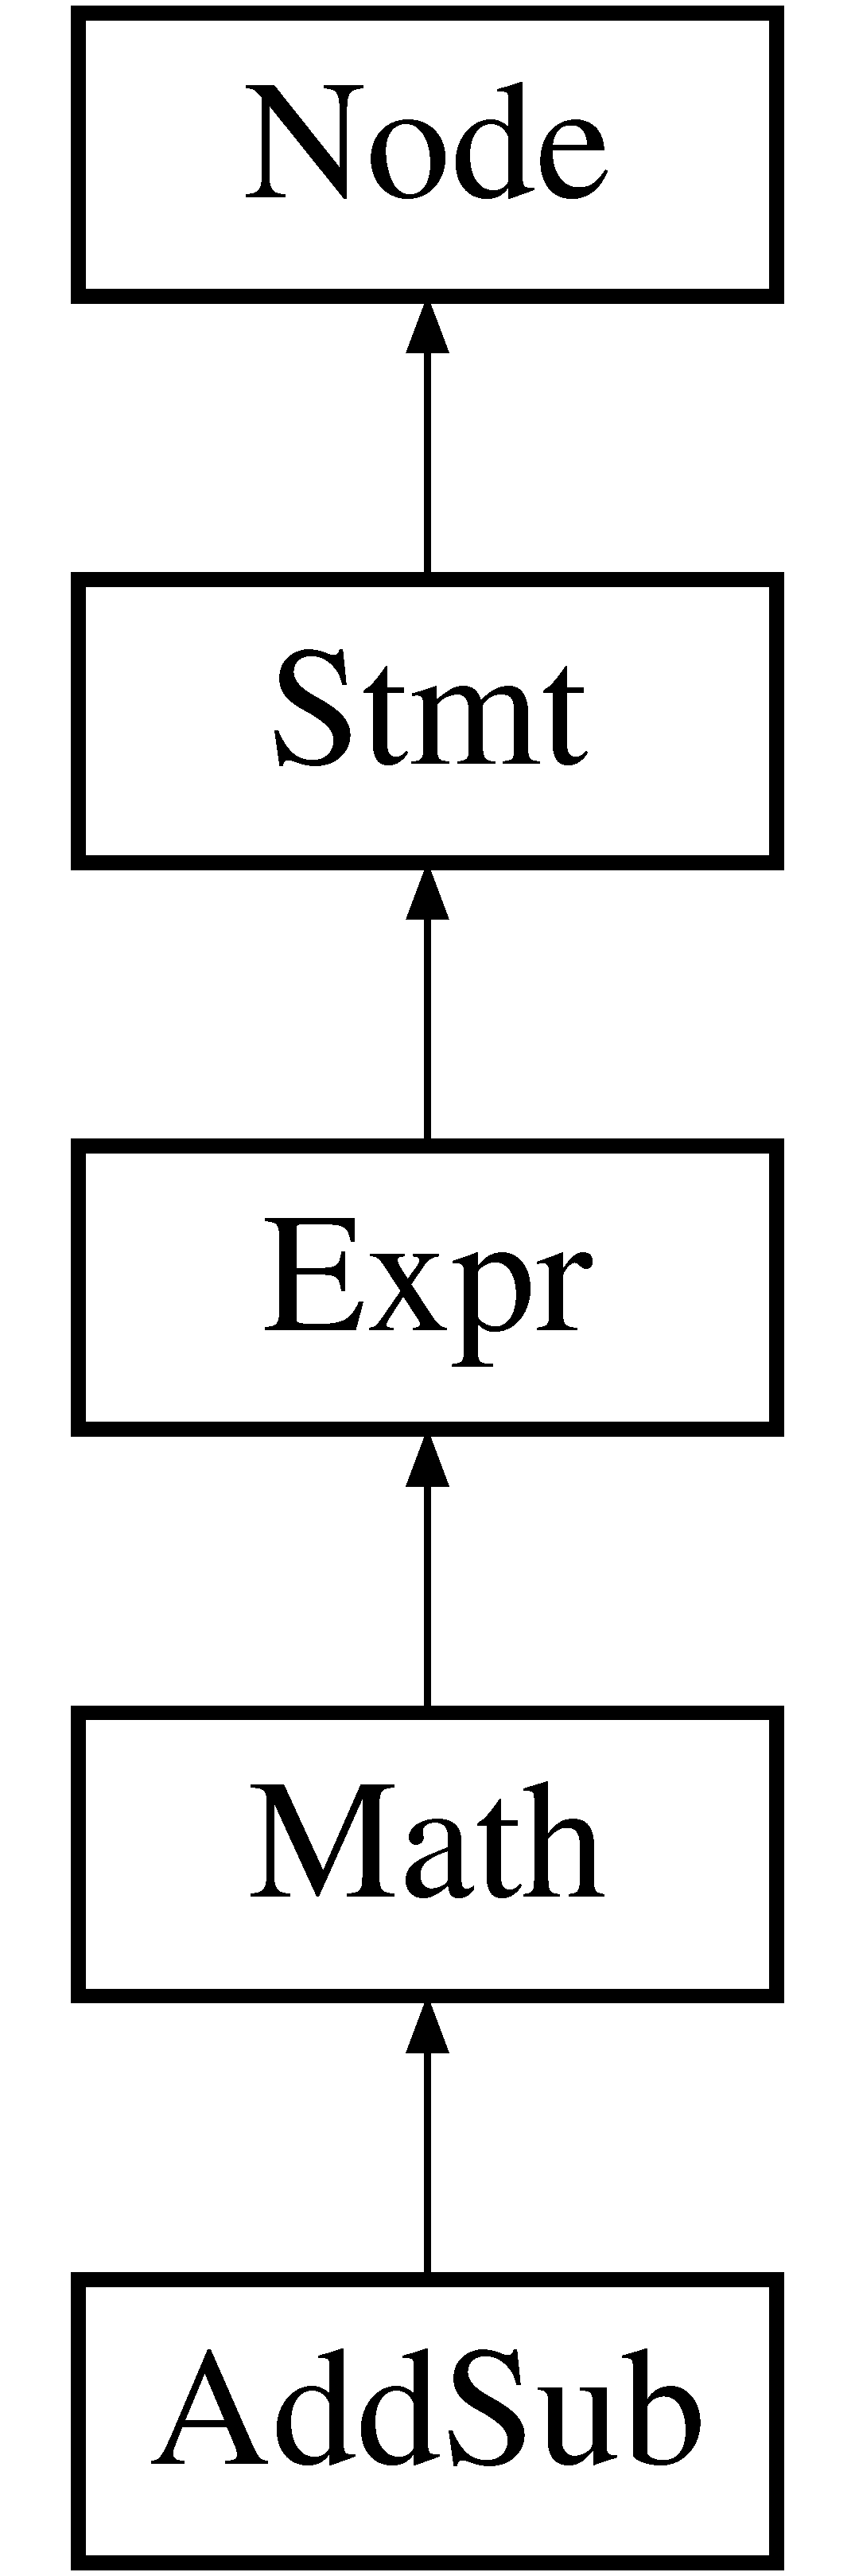
\includegraphics[height=5.000000cm]{class_add_sub}
\end{center}
\end{figure}
\subsection*{Public 成员函数}
\begin{DoxyCompactItemize}
\item 
\hyperlink{class_add_sub_af090ec4bb8a06ee586c4bfa8f4bad3ef}{Add\+Sub} (\hyperlink{class_token}{Token} $\ast$token, \hyperlink{class_expr}{Expr} $\ast$expr1, \hyperlink{class_expr}{Expr} $\ast$expr2)
\item 
int \hyperlink{class_add_sub_a73c0513a31a5400fdfc79ce877a1c3b9}{execute} ()
\end{DoxyCompactItemize}
\subsection*{额外继承的成员函数}


\subsection{详细描述}
加减表达式类 

\subsection{构造及析构函数说明}
\index{Add\+Sub@{Add\+Sub}!Add\+Sub@{Add\+Sub}}
\index{Add\+Sub@{Add\+Sub}!Add\+Sub@{Add\+Sub}}
\subsubsection[{\texorpdfstring{Add\+Sub(\+Token $\ast$token, Expr $\ast$expr1, Expr $\ast$expr2)}{AddSub(Token *token, Expr *expr1, Expr *expr2)}}]{\setlength{\rightskip}{0pt plus 5cm}Add\+Sub\+::\+Add\+Sub (
\begin{DoxyParamCaption}
\item[{{\bf Token} $\ast$}]{token, }
\item[{{\bf Expr} $\ast$}]{expr1, }
\item[{{\bf Expr} $\ast$}]{expr2}
\end{DoxyParamCaption}
)}\hypertarget{class_add_sub_af090ec4bb8a06ee586c4bfa8f4bad3ef}{}\label{class_add_sub_af090ec4bb8a06ee586c4bfa8f4bad3ef}

\begin{DoxyParams}{参数}
{\em token} & \+: 运算符的 token \\
\hline
{\em expr1} & \+: 左表达式 \\
\hline
{\em expr2} & \+: 右表达式 \\
\hline
\end{DoxyParams}


\subsection{成员函数说明}
\index{Add\+Sub@{Add\+Sub}!execute@{execute}}
\index{execute@{execute}!Add\+Sub@{Add\+Sub}}
\subsubsection[{\texorpdfstring{execute()}{execute()}}]{\setlength{\rightskip}{0pt plus 5cm}int Add\+Sub\+::execute (
\begin{DoxyParamCaption}
{}
\end{DoxyParamCaption}
)\hspace{0.3cm}{\ttfamily [virtual]}}\hypertarget{class_add_sub_a73c0513a31a5400fdfc79ce877a1c3b9}{}\label{class_add_sub_a73c0513a31a5400fdfc79ce877a1c3b9}
\begin{DoxyReturn}{返回}
运算后的值 
\end{DoxyReturn}


重载 \hyperlink{class_expr_aff6a2e6eaa460e2a3db28ebdab089b51}{Expr} .



该类的文档由以下文件生成\+:\begin{DoxyCompactItemize}
\item 
src/inter/stmt/expr/Add\+Sub.\+h\item 
src/inter/stmt/expr/Add\+Sub.\+cpp\end{DoxyCompactItemize}

\hypertarget{class_blank}{}\section{Blank Class Reference}
\label{class_blank}\index{Blank@{Blank}}


空语句类  




{\ttfamily \#include $<$Blank.\+h$>$}

Inheritance diagram for Blank\+:\begin{figure}[H]
\begin{center}
\leavevmode
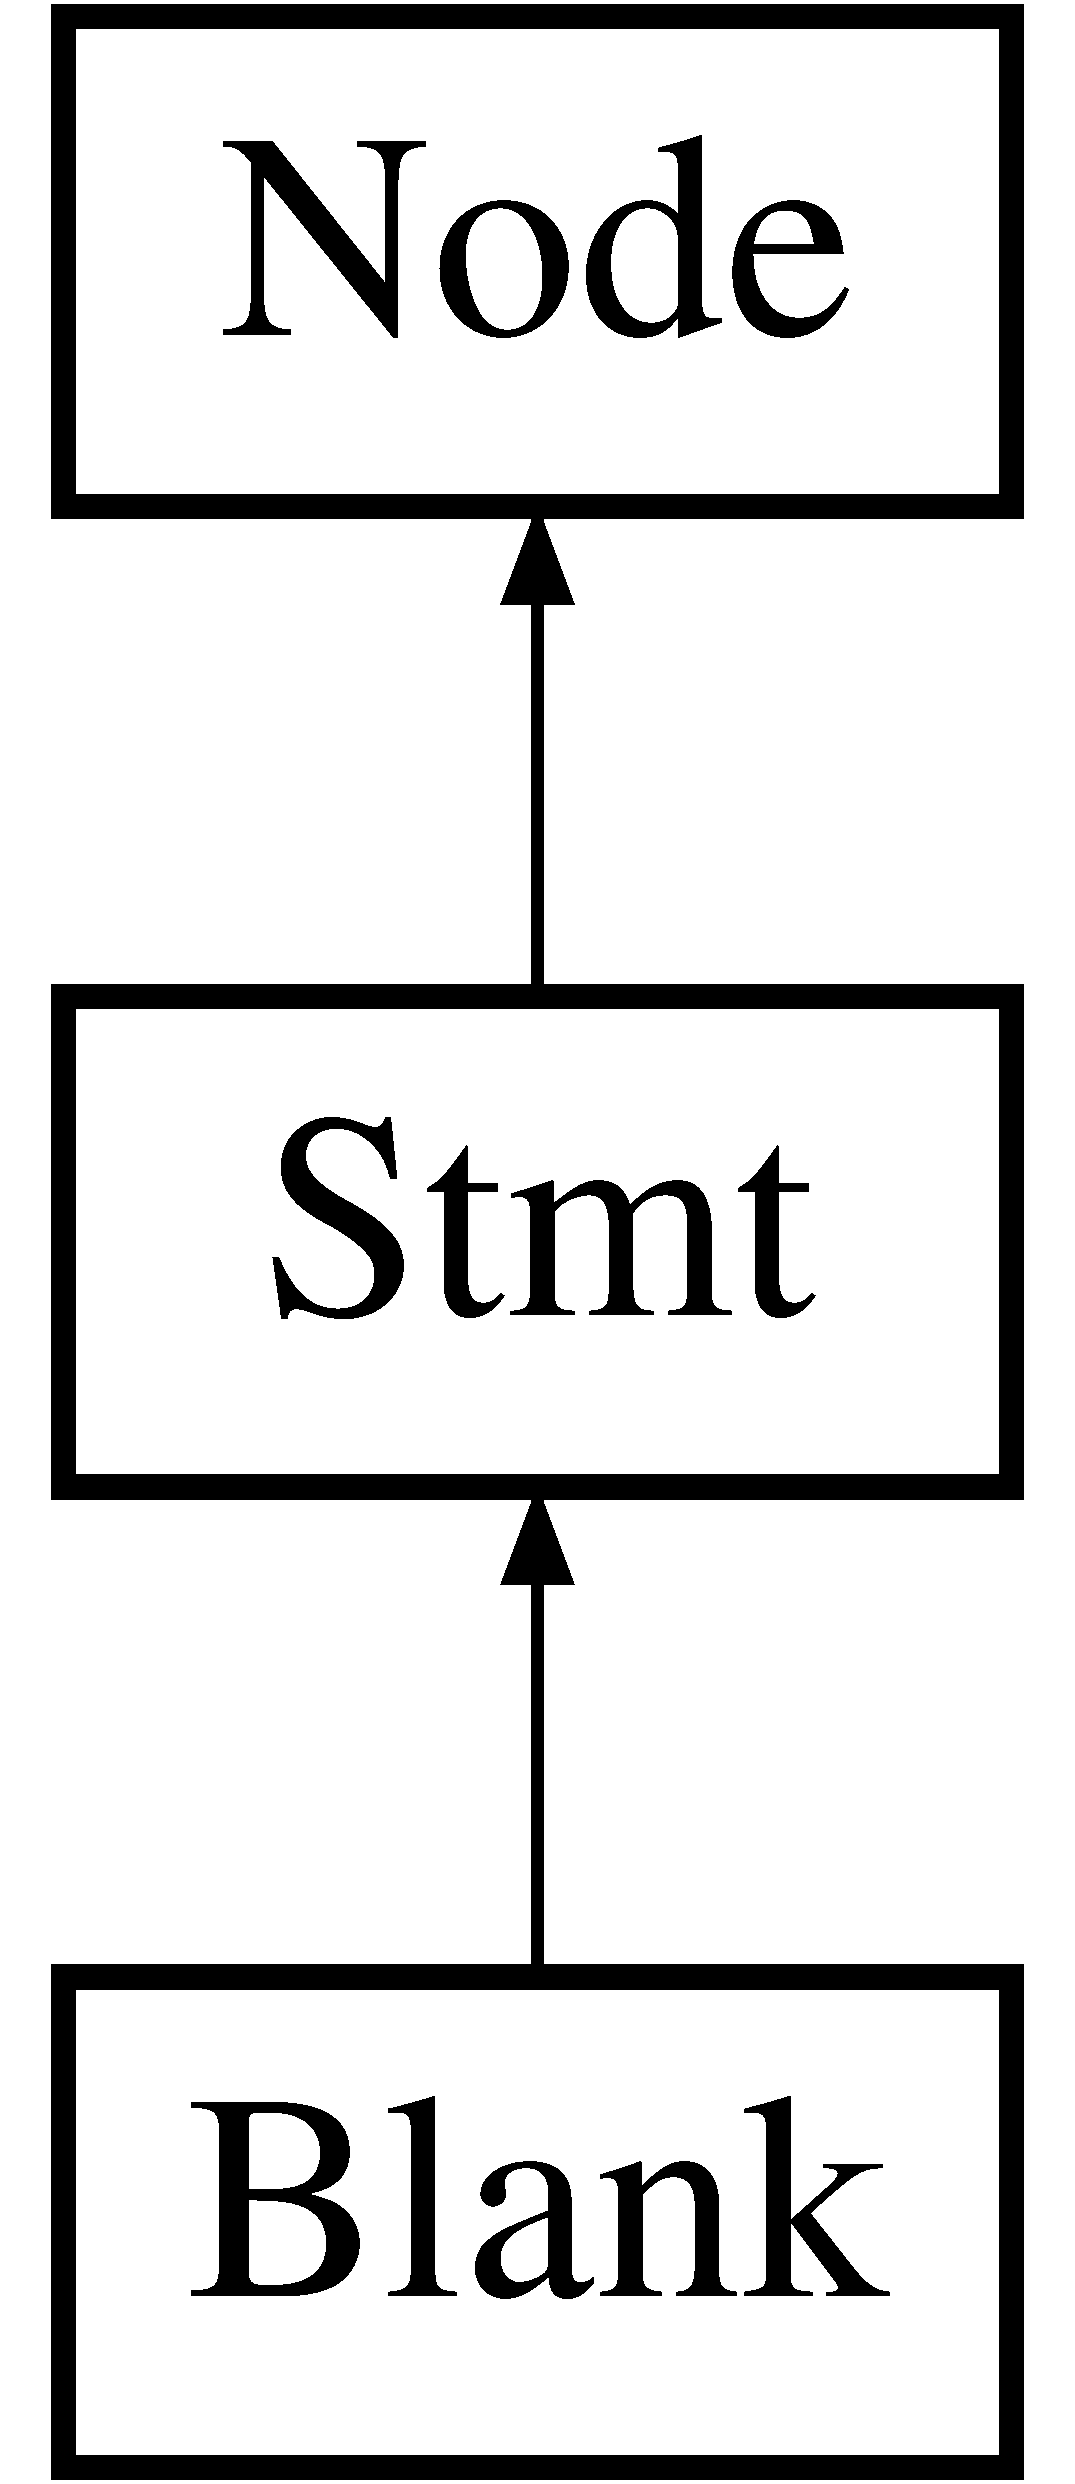
\includegraphics[height=3.000000cm]{class_blank}
\end{center}
\end{figure}
\subsection*{Additional Inherited Members}


\subsection{Detailed Description}
空语句类 

The documentation for this class was generated from the following file\+:\begin{DoxyCompactItemize}
\item 
src/inter/stmt/Blank.\+h\end{DoxyCompactItemize}

\hypertarget{class_block}{}\section{Block Class Reference}
\label{class_block}\index{Block@{Block}}


{\ttfamily \#include $<$Block.\+h$>$}

Inheritance diagram for Block\+:\begin{figure}[H]
\begin{center}
\leavevmode
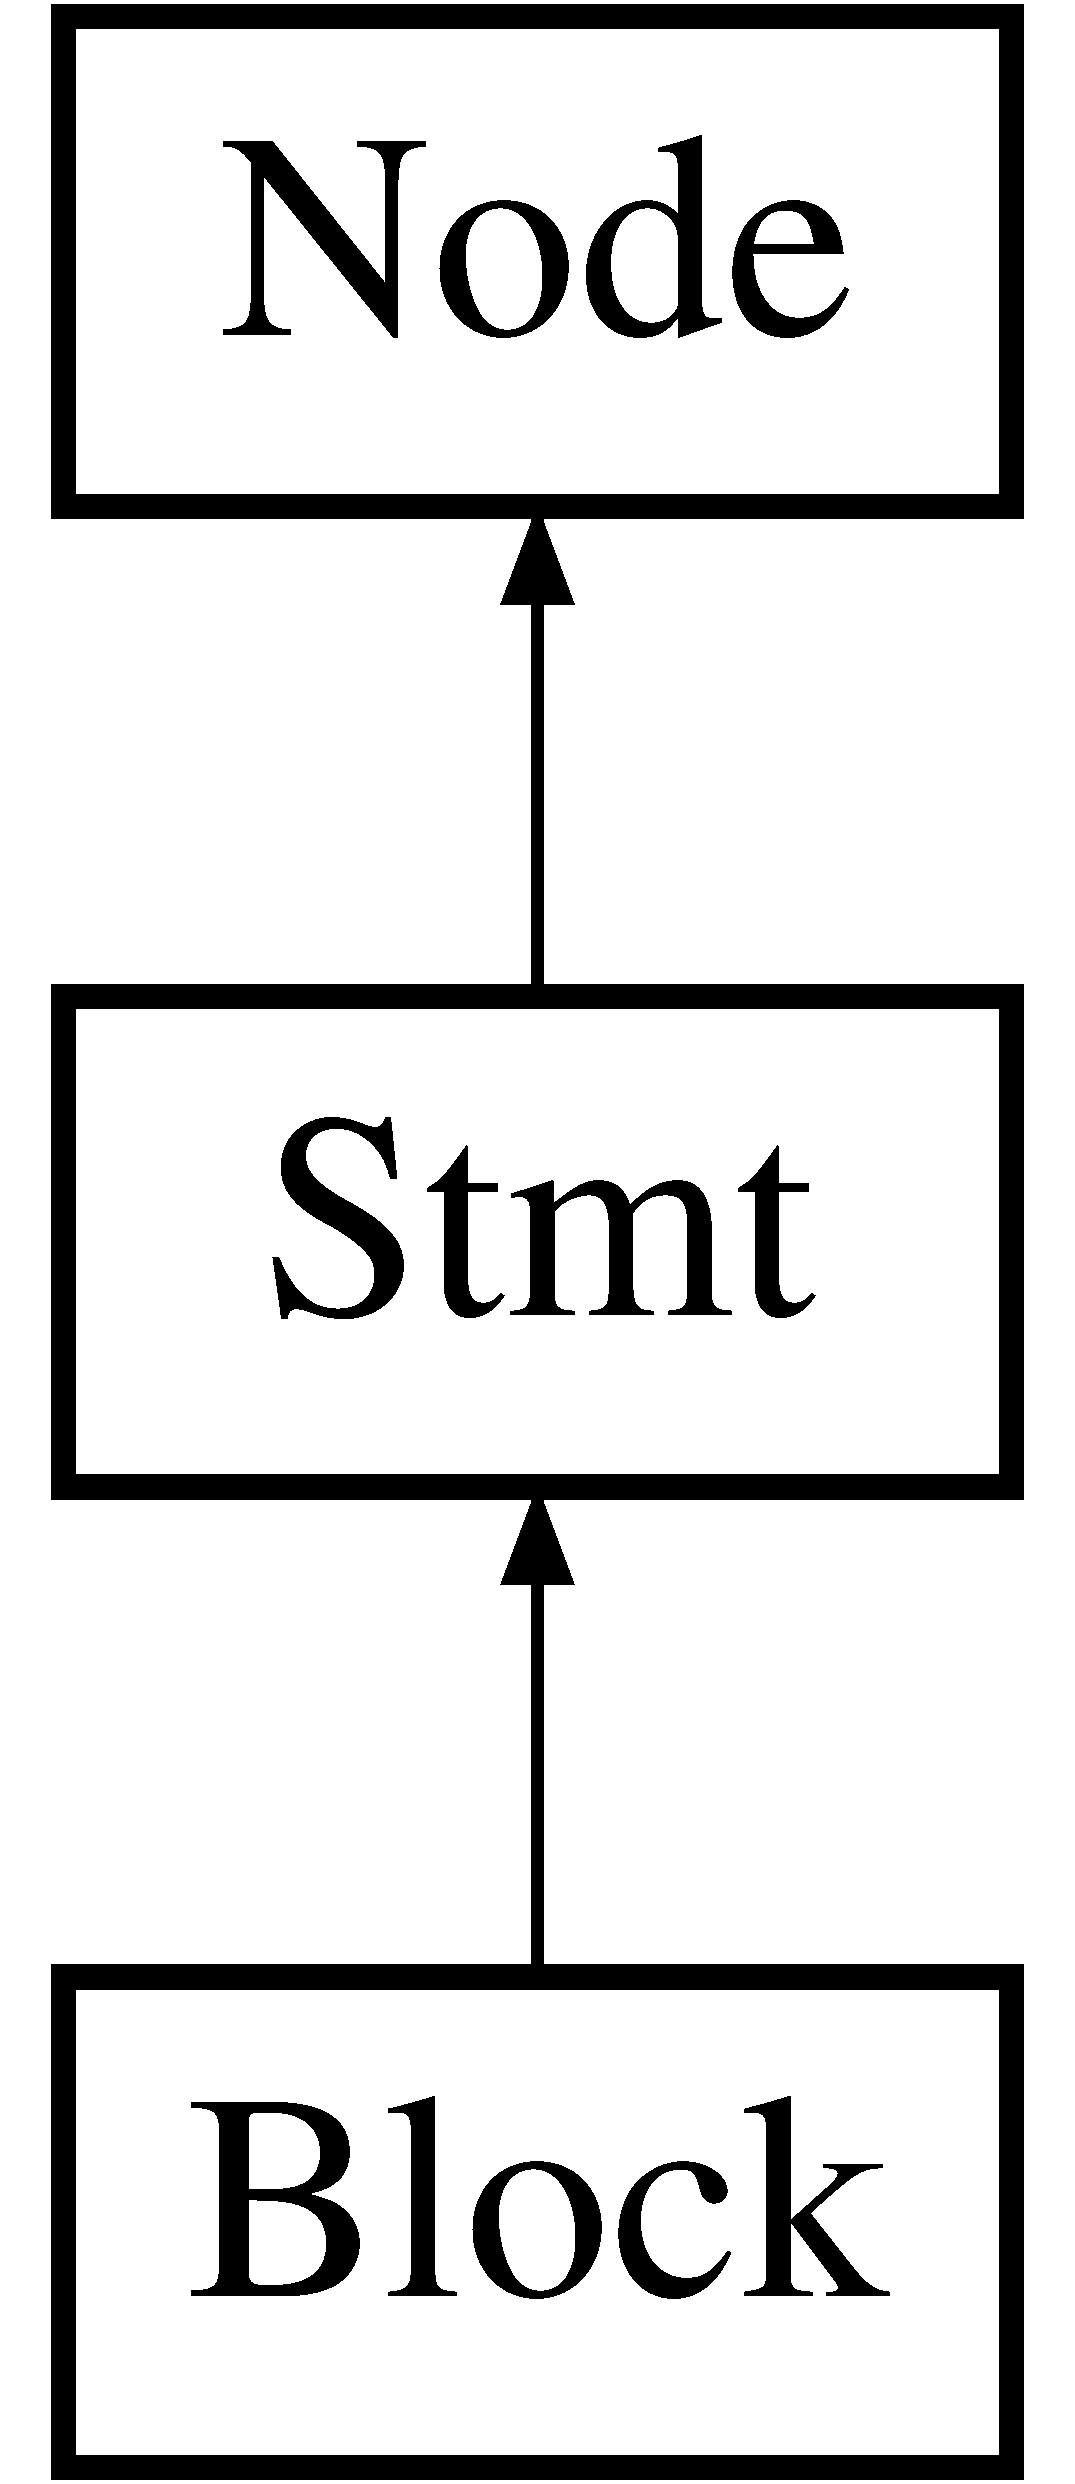
\includegraphics[height=3.000000cm]{class_block}
\end{center}
\end{figure}
\subsection*{Public Member Functions}
\begin{DoxyCompactItemize}
\item 
int \hyperlink{class_block_a8e03f15df4e43cd6c802341c3bda6b33}{execute} ()
\begin{DoxyCompactList}\small\item\em 抽象的执行方法 \end{DoxyCompactList}\item 
void \hyperlink{class_block_aa48058bd426766898bf31df828b3dac2}{set\+Env} (\hyperlink{class_env}{Env} $\ast$)
\item 
void \hyperlink{class_block_acd012454c035cc7e0d508365752221ff}{push\+\_\+stmt} (\hyperlink{class_stmt}{Stmt} $\ast$)
\end{DoxyCompactItemize}
\subsection*{Public Attributes}
\begin{DoxyCompactItemize}
\item 
std\+::vector$<$ \hyperlink{class_break}{Break} $\ast$ $>$ \hyperlink{class_block_a8cdf287fcbcf92cc429c78b79464b363}{breaks}
\end{DoxyCompactItemize}
\subsection*{Protected Attributes}
\begin{DoxyCompactItemize}
\item 
std\+::vector$<$ \hyperlink{class_stmt}{Stmt} $\ast$ $>$ \hyperlink{class_block_a88f627f956bdc80d9d697f0755130d34}{stmts}
\item 
\hyperlink{class_env}{Env} $\ast$ \hyperlink{class_block_a85617f1e8f9f4b998e9b1ebc4c3b37c4}{env}
\end{DoxyCompactItemize}
\subsection*{Additional Inherited Members}


\subsection{Member Function Documentation}
\mbox{\Hypertarget{class_block_a8e03f15df4e43cd6c802341c3bda6b33}\label{class_block_a8e03f15df4e43cd6c802341c3bda6b33}} 
\index{Block@{Block}!execute@{execute}}
\index{execute@{execute}!Block@{Block}}
\subsubsection{\texorpdfstring{execute()}{execute()}}
{\footnotesize\ttfamily int Block\+::execute (\begin{DoxyParamCaption}{ }\end{DoxyParamCaption})\hspace{0.3cm}{\ttfamily [virtual]}}



抽象的执行方法 

因为表达式以及各种语句都是可执行的~\newline
设立这个方法利用多态可以实现整个语法树的执行~\newline
 \begin{DoxyReturn}{Returns}
int \+: 表达式或语句执行后获得的值 
\end{DoxyReturn}


Reimplemented from \hyperlink{class_stmt_abdc3261770c3c5bd3ce5b3ba6eedfaa4}{Stmt}.

\mbox{\Hypertarget{class_block_acd012454c035cc7e0d508365752221ff}\label{class_block_acd012454c035cc7e0d508365752221ff}} 
\index{Block@{Block}!push\+\_\+stmt@{push\+\_\+stmt}}
\index{push\+\_\+stmt@{push\+\_\+stmt}!Block@{Block}}
\subsubsection{\texorpdfstring{push\+\_\+stmt()}{push\_stmt()}}
{\footnotesize\ttfamily void Block\+::push\+\_\+stmt (\begin{DoxyParamCaption}\item[{\hyperlink{class_stmt}{Stmt} $\ast$}]{stmt }\end{DoxyParamCaption})}

\mbox{\Hypertarget{class_block_aa48058bd426766898bf31df828b3dac2}\label{class_block_aa48058bd426766898bf31df828b3dac2}} 
\index{Block@{Block}!set\+Env@{set\+Env}}
\index{set\+Env@{set\+Env}!Block@{Block}}
\subsubsection{\texorpdfstring{set\+Env()}{setEnv()}}
{\footnotesize\ttfamily void Block\+::set\+Env (\begin{DoxyParamCaption}\item[{\hyperlink{class_env}{Env} $\ast$}]{env }\end{DoxyParamCaption})}



\subsection{Member Data Documentation}
\mbox{\Hypertarget{class_block_a8cdf287fcbcf92cc429c78b79464b363}\label{class_block_a8cdf287fcbcf92cc429c78b79464b363}} 
\index{Block@{Block}!breaks@{breaks}}
\index{breaks@{breaks}!Block@{Block}}
\subsubsection{\texorpdfstring{breaks}{breaks}}
{\footnotesize\ttfamily std\+::vector$<$\hyperlink{class_break}{Break}$\ast$$>$ Block\+::breaks}

\mbox{\Hypertarget{class_block_a85617f1e8f9f4b998e9b1ebc4c3b37c4}\label{class_block_a85617f1e8f9f4b998e9b1ebc4c3b37c4}} 
\index{Block@{Block}!env@{env}}
\index{env@{env}!Block@{Block}}
\subsubsection{\texorpdfstring{env}{env}}
{\footnotesize\ttfamily \hyperlink{class_env}{Env}$\ast$ Block\+::env\hspace{0.3cm}{\ttfamily [protected]}}

\mbox{\Hypertarget{class_block_a88f627f956bdc80d9d697f0755130d34}\label{class_block_a88f627f956bdc80d9d697f0755130d34}} 
\index{Block@{Block}!stmts@{stmts}}
\index{stmts@{stmts}!Block@{Block}}
\subsubsection{\texorpdfstring{stmts}{stmts}}
{\footnotesize\ttfamily std\+::vector$<$\hyperlink{class_stmt}{Stmt} $\ast$$>$ Block\+::stmts\hspace{0.3cm}{\ttfamily [protected]}}



The documentation for this class was generated from the following files\+:\begin{DoxyCompactItemize}
\item 
src/inter/stmt/\hyperlink{_block_8h}{Block.\+h}\item 
src/inter/stmt/\hyperlink{_block_8cpp}{Block.\+cpp}\end{DoxyCompactItemize}

\hypertarget{class_break}{}\section{Break类 参考}
\label{class_break}\index{Break@{Break}}


循环中断类  




{\ttfamily \#include $<$Break.\+h$>$}

类 Break 继承关系图\+:\begin{figure}[H]
\begin{center}
\leavevmode
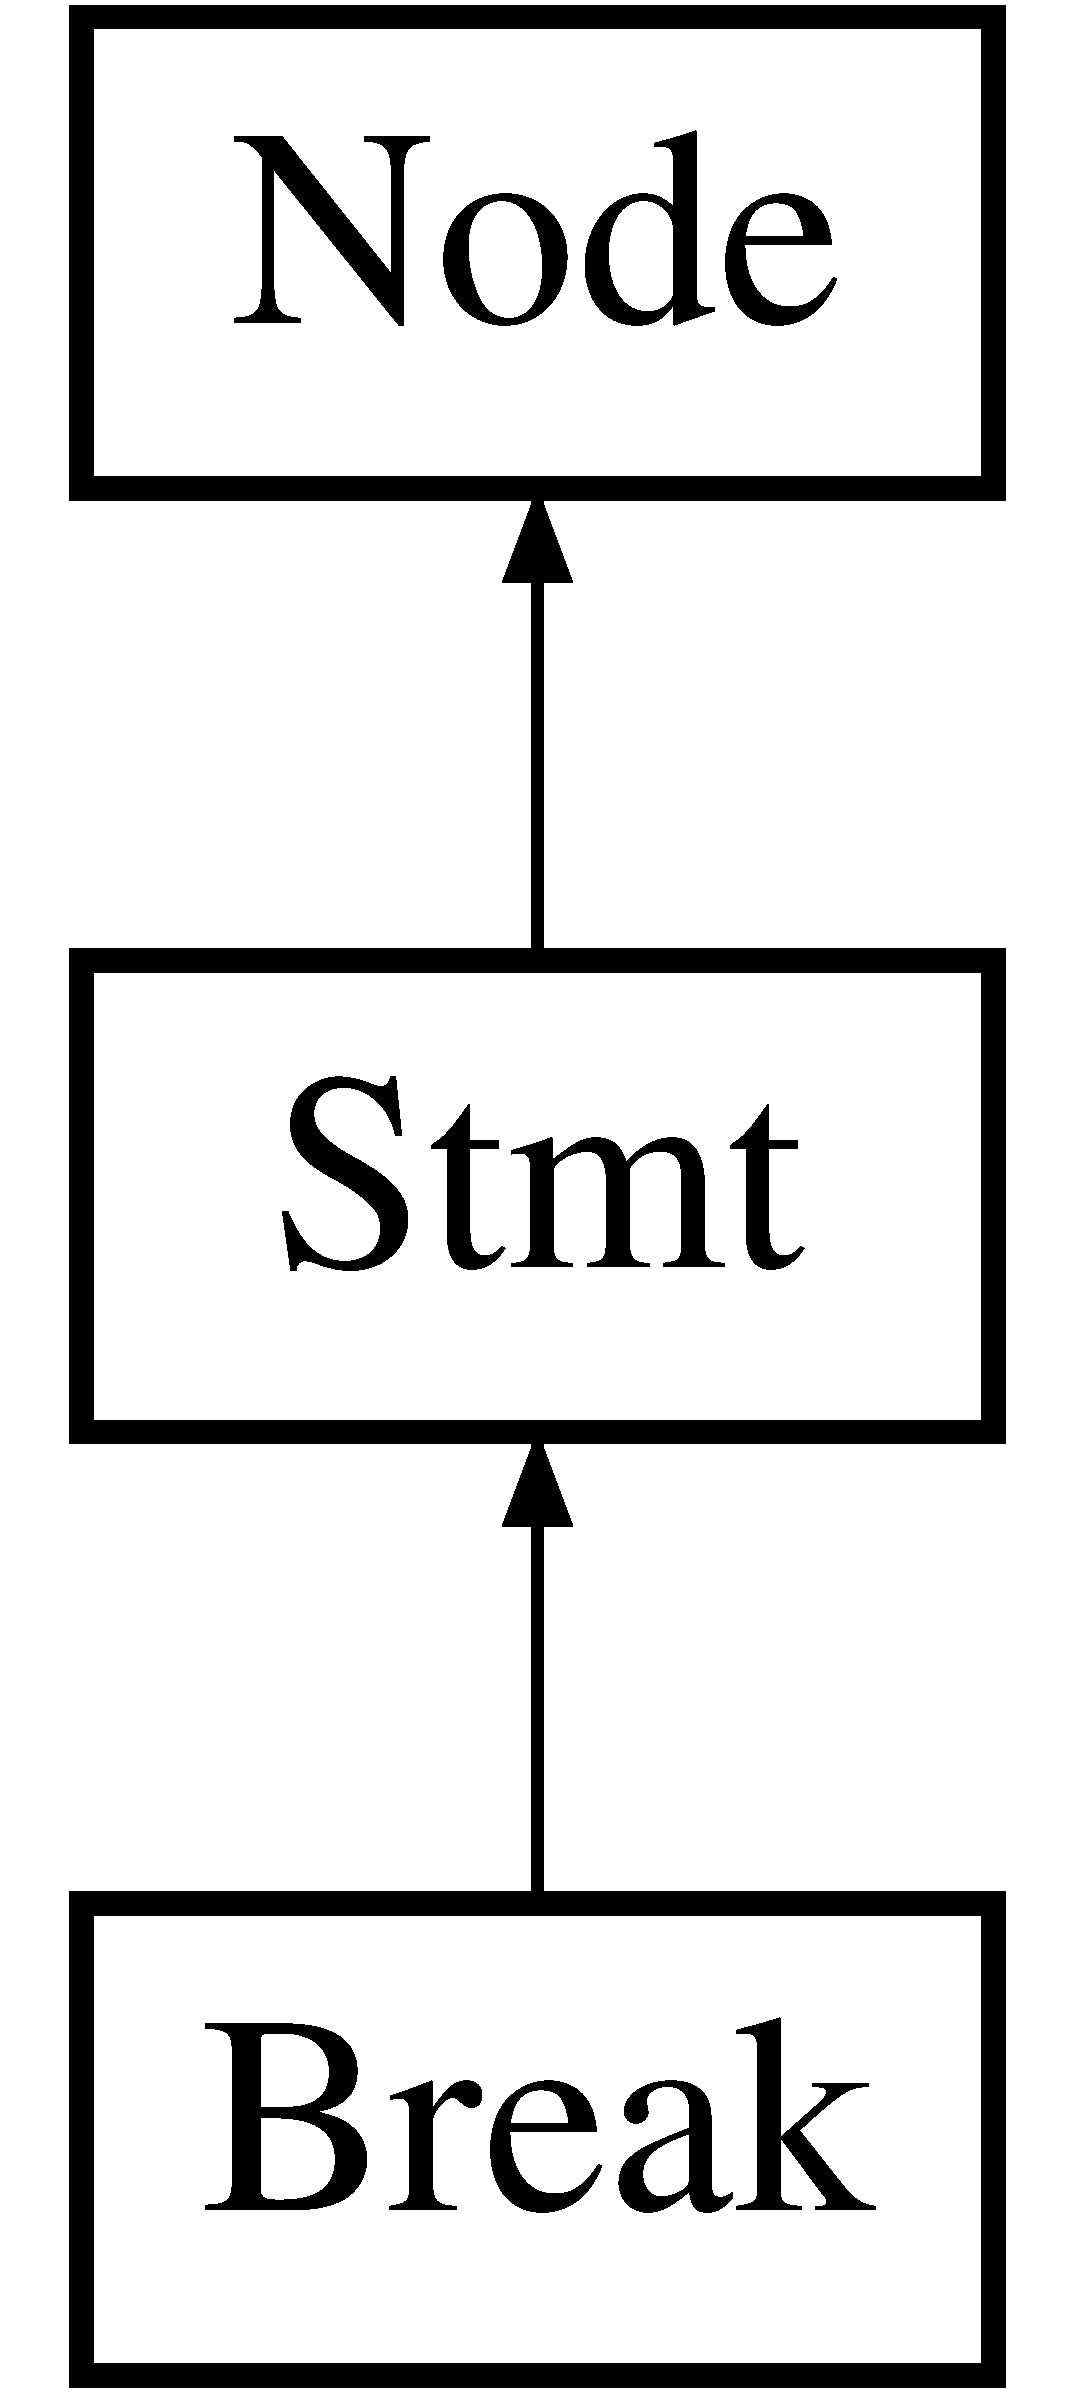
\includegraphics[height=3.000000cm]{class_break}
\end{center}
\end{figure}
\subsection*{Public 成员函数}
\begin{DoxyCompactItemize}
\item 
\mbox{\Hypertarget{class_break_a554fd4cae05d203145d62868f73004d4}\label{class_break_a554fd4cae05d203145d62868f73004d4}} 
int \hyperlink{class_break_a554fd4cae05d203145d62868f73004d4}{execute} ()
\begin{DoxyCompactList}\small\item\em 执行循环中断,抛出中断异常 \end{DoxyCompactList}\end{DoxyCompactItemize}
\subsection*{额外继承的成员函数}


\subsection{详细描述}
循环中断类 

该类的文档由以下文件生成\+:\begin{DoxyCompactItemize}
\item 
src/inter/stmt/Break.\+h\item 
src/inter/stmt/Break.\+cpp\end{DoxyCompactItemize}

\hypertarget{class_break_error}{}\section{Break\+Error Class Reference}
\label{class_break_error}\index{Break\+Error@{Break\+Error}}


Break类  




{\ttfamily \#include $<$Break\+Error.\+h$>$}

Inheritance diagram for Break\+Error\+:\begin{figure}[H]
\begin{center}
\leavevmode
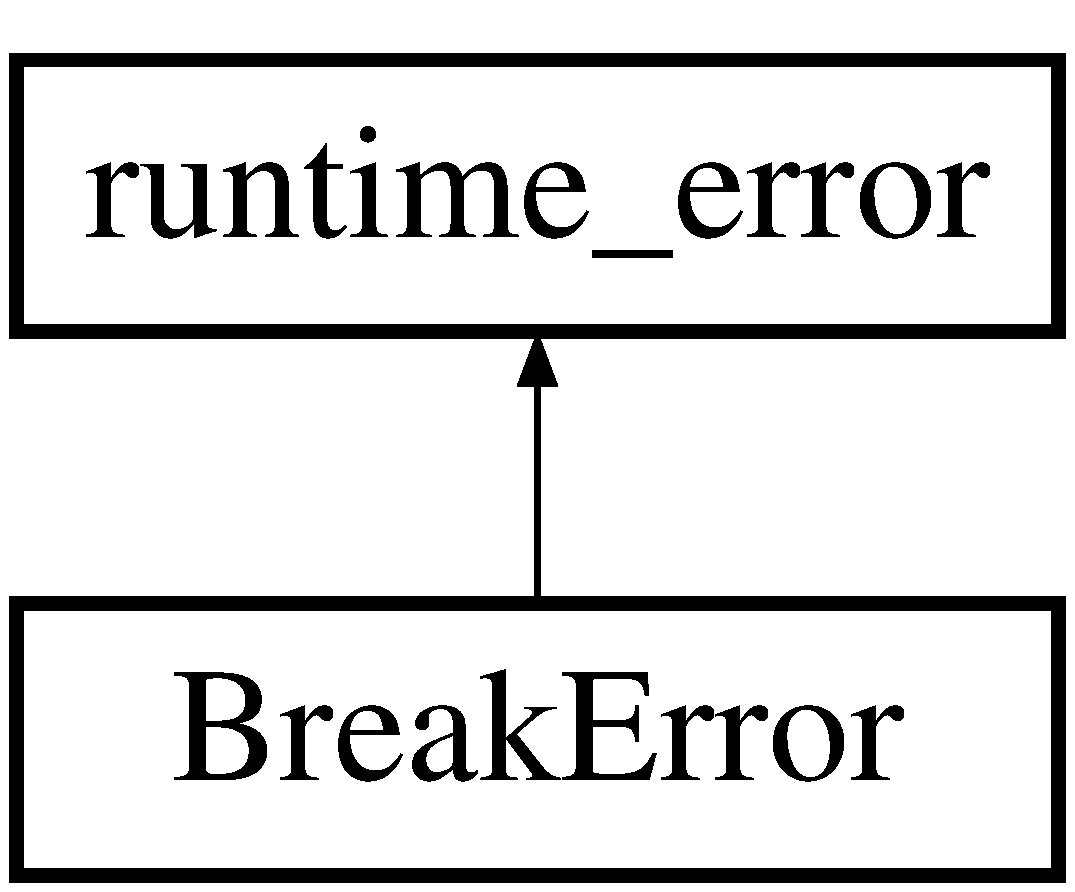
\includegraphics[height=2.000000cm]{class_break_error}
\end{center}
\end{figure}
\subsection*{Public Member Functions}
\begin{DoxyCompactItemize}
\item 
\mbox{\Hypertarget{class_break_error_a94dc77c2e9e9088a44b073a9eda03833}\label{class_break_error_a94dc77c2e9e9088a44b073a9eda03833}} 
{\bfseries Break\+Error} (std\+::string)
\end{DoxyCompactItemize}


\subsection{Detailed Description}
Break类 

用于抛出break的异常~\newline
便于\+While循环提前中断 

The documentation for this class was generated from the following files\+:\begin{DoxyCompactItemize}
\item 
src/inter/error/Break\+Error.\+h\item 
src/inter/error/Break\+Error.\+cpp\end{DoxyCompactItemize}

\hypertarget{class_comma}{}\section{Comma Class Reference}
\label{class_comma}\index{Comma@{Comma}}


逗号表达式类  




{\ttfamily \#include $<$Comma.\+h$>$}

Inheritance diagram for Comma\+:\begin{figure}[H]
\begin{center}
\leavevmode
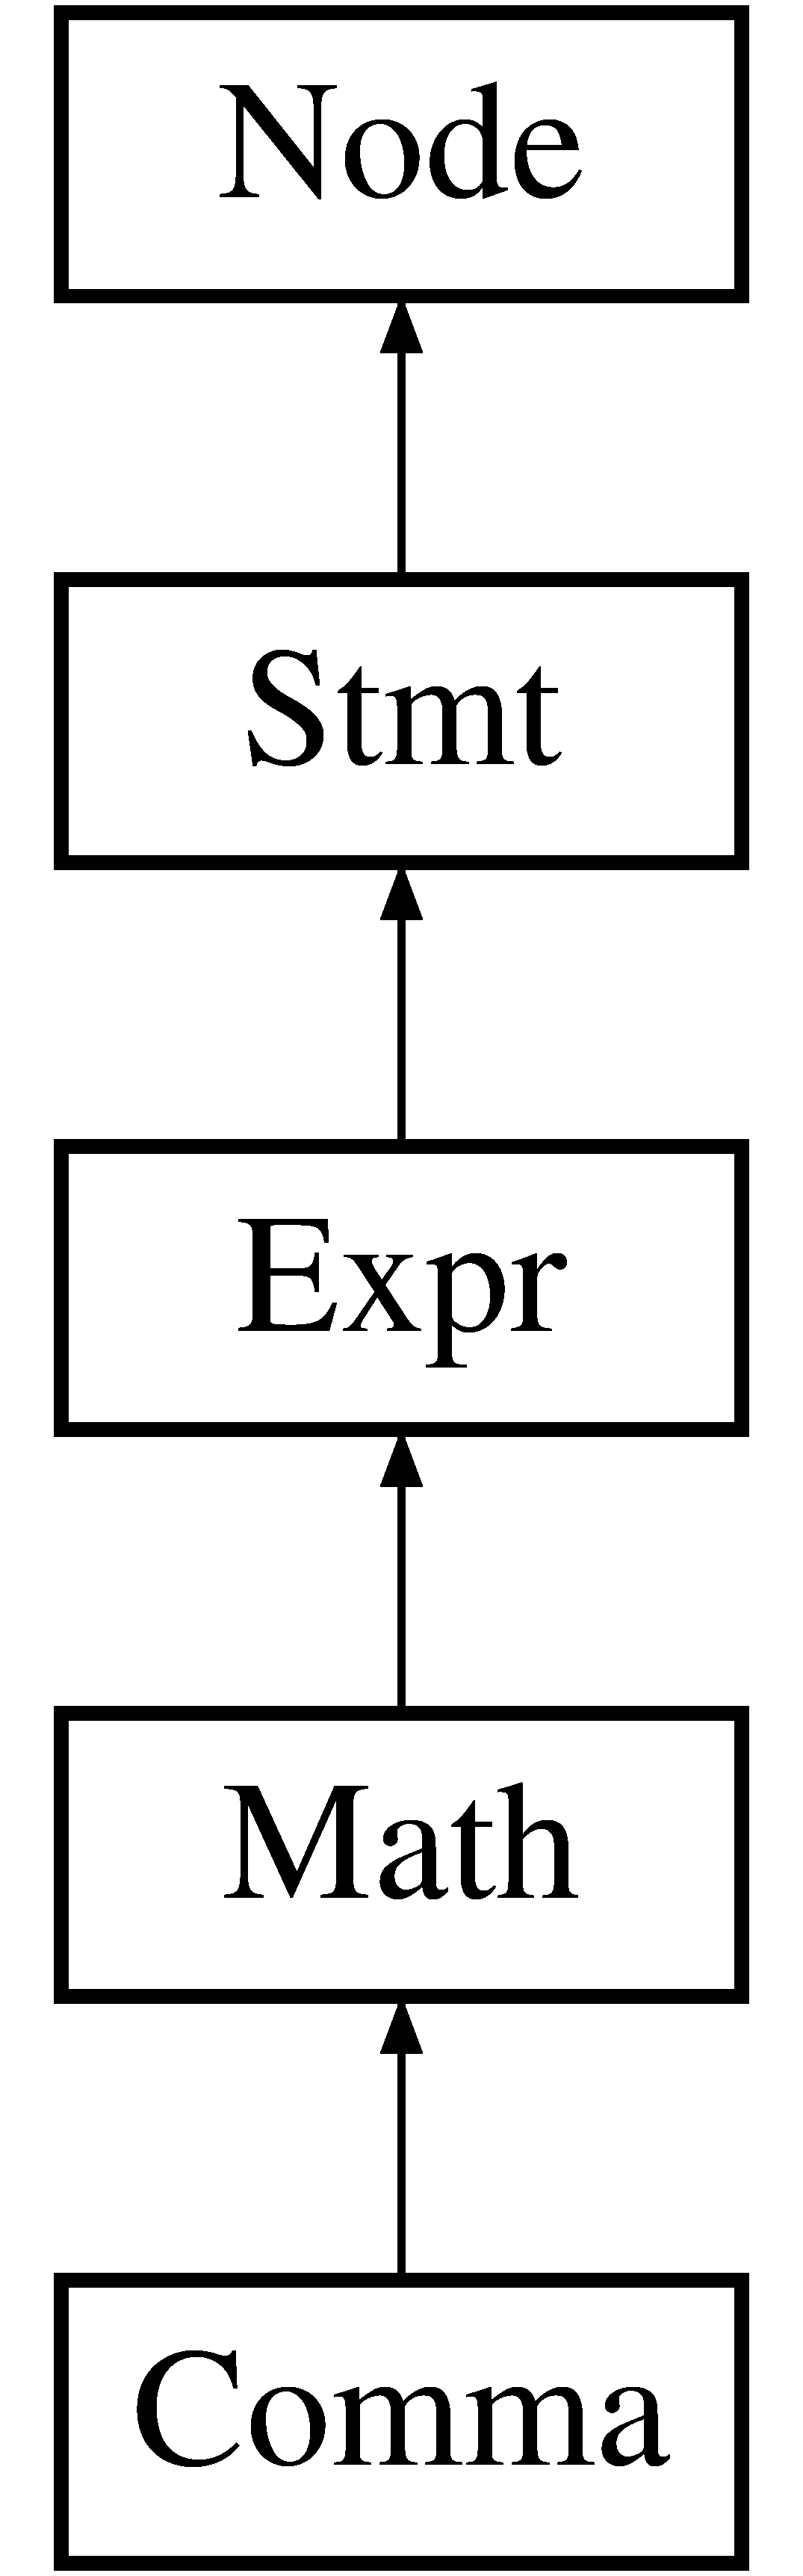
\includegraphics[height=5.000000cm]{class_comma}
\end{center}
\end{figure}
\subsection*{Public Member Functions}
\begin{DoxyCompactItemize}
\item 
\hyperlink{class_comma_a53c0fef57ecec72be524b054ab6b3ae6}{Comma} (\hyperlink{class_token}{Token} $\ast$, \hyperlink{class_expr}{Expr} $\ast$, \hyperlink{class_expr}{Expr} $\ast$)
\item 
int \hyperlink{class_comma_aab9ca2bb70a10abd2fb263de745f843a}{execute} ()
\end{DoxyCompactItemize}
\subsection*{Additional Inherited Members}


\subsection{Detailed Description}
逗号表达式类 

\subsection{Constructor \& Destructor Documentation}
\mbox{\Hypertarget{class_comma_a53c0fef57ecec72be524b054ab6b3ae6}\label{class_comma_a53c0fef57ecec72be524b054ab6b3ae6}} 
\index{Comma@{Comma}!Comma@{Comma}}
\index{Comma@{Comma}!Comma@{Comma}}
\subsubsection{\texorpdfstring{Comma()}{Comma()}}
{\footnotesize\ttfamily Comma\+::\+Comma (\begin{DoxyParamCaption}\item[{\hyperlink{class_token}{Token} $\ast$}]{token,  }\item[{\hyperlink{class_expr}{Expr} $\ast$}]{expr1,  }\item[{\hyperlink{class_expr}{Expr} $\ast$}]{expr2 }\end{DoxyParamCaption})}


\begin{DoxyParams}{Parameters}
{\em token} & \+: 逗号的 token \\
\hline
{\em expr1} & \+: 左表达式 \\
\hline
{\em expr2} & \+: 右表达式 \\
\hline
\end{DoxyParams}


\subsection{Member Function Documentation}
\mbox{\Hypertarget{class_comma_aab9ca2bb70a10abd2fb263de745f843a}\label{class_comma_aab9ca2bb70a10abd2fb263de745f843a}} 
\index{Comma@{Comma}!execute@{execute}}
\index{execute@{execute}!Comma@{Comma}}
\subsubsection{\texorpdfstring{execute()}{execute()}}
{\footnotesize\ttfamily int Comma\+::execute (\begin{DoxyParamCaption}{ }\end{DoxyParamCaption})\hspace{0.3cm}{\ttfamily [virtual]}}

\begin{DoxyReturn}{Returns}
右表达式的值 
\end{DoxyReturn}


Reimplemented from \hyperlink{class_expr_aff6a2e6eaa460e2a3db28ebdab089b51}{Expr}.



The documentation for this class was generated from the following files\+:\begin{DoxyCompactItemize}
\item 
src/inter/stmt/expr/Comma.\+h\item 
src/inter/stmt/expr/Comma.\+cpp\end{DoxyCompactItemize}

\hypertarget{class_constant}{}\section{Constant类 参考}
\label{class_constant}\index{Constant@{Constant}}


常数类  




{\ttfamily \#include $<$Constant.\+h$>$}

类 Constant 继承关系图\+:\begin{figure}[H]
\begin{center}
\leavevmode
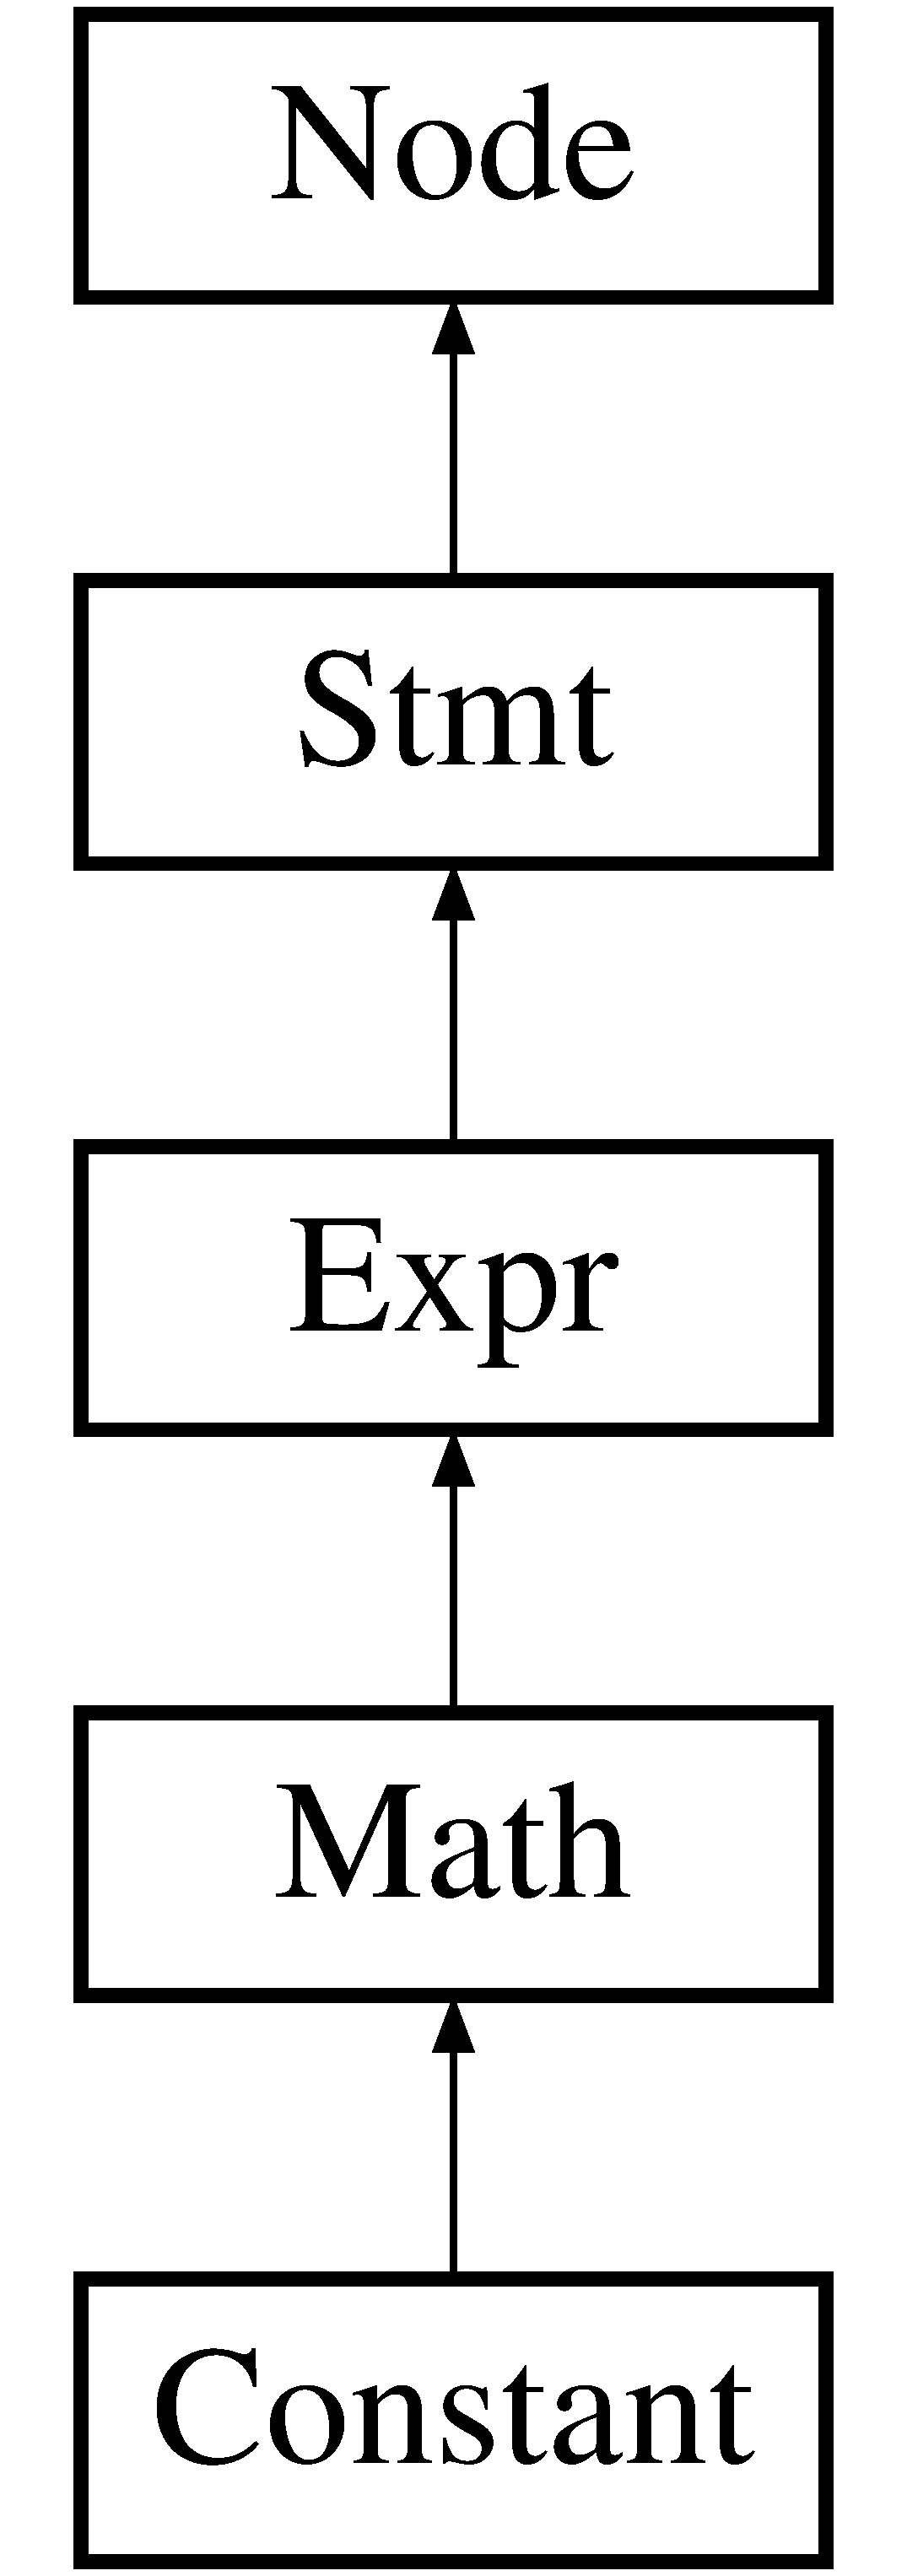
\includegraphics[height=5.000000cm]{class_constant}
\end{center}
\end{figure}
\subsection*{Public 成员函数}
\begin{DoxyCompactItemize}
\item 
\hyperlink{class_constant_ad227bb35513aab43d86572343a1fe564}{Constant} (\hyperlink{class_token}{Token} $\ast$)
\item 
int \hyperlink{class_constant_ab5c55607bcff5ce70131a588b6bdbed7}{execute} ()
\end{DoxyCompactItemize}
\subsection*{Public 属性}
\begin{DoxyCompactItemize}
\item 
int \hyperlink{class_constant_a132c9bc0ec98681bcbf723d87ddd722d}{value}
\end{DoxyCompactItemize}
\subsection*{额外继承的成员函数}


\subsection{详细描述}
常数类 

\subsection{构造及析构函数说明}
\mbox{\Hypertarget{class_constant_ad227bb35513aab43d86572343a1fe564}\label{class_constant_ad227bb35513aab43d86572343a1fe564}} 
\index{Constant@{Constant}!Constant@{Constant}}
\index{Constant@{Constant}!Constant@{Constant}}
\subsubsection{\texorpdfstring{Constant()}{Constant()}}
{\footnotesize\ttfamily Constant\+::\+Constant (\begin{DoxyParamCaption}\item[{\hyperlink{class_token}{Token} $\ast$}]{token }\end{DoxyParamCaption})}


\begin{DoxyParams}{参数}
{\em token} & \+: 该常数的 token \\
\hline
\end{DoxyParams}


\subsection{成员函数说明}
\mbox{\Hypertarget{class_constant_ab5c55607bcff5ce70131a588b6bdbed7}\label{class_constant_ab5c55607bcff5ce70131a588b6bdbed7}} 
\index{Constant@{Constant}!execute@{execute}}
\index{execute@{execute}!Constant@{Constant}}
\subsubsection{\texorpdfstring{execute()}{execute()}}
{\footnotesize\ttfamily int Constant\+::execute (\begin{DoxyParamCaption}{ }\end{DoxyParamCaption})\hspace{0.3cm}{\ttfamily [virtual]}}

\begin{DoxyReturn}{返回}
常数的值 
\end{DoxyReturn}


重载 \hyperlink{class_expr_aff6a2e6eaa460e2a3db28ebdab089b51}{Expr} .



\subsection{类成员变量说明}
\mbox{\Hypertarget{class_constant_a132c9bc0ec98681bcbf723d87ddd722d}\label{class_constant_a132c9bc0ec98681bcbf723d87ddd722d}} 
\index{Constant@{Constant}!value@{value}}
\index{value@{value}!Constant@{Constant}}
\subsubsection{\texorpdfstring{value}{value}}
{\footnotesize\ttfamily int Constant\+::value}

常数的值 

该类的文档由以下文件生成\+:\begin{DoxyCompactItemize}
\item 
src/inter/stmt/expr/Constant.\+h\item 
src/inter/stmt/expr/Constant.\+cpp\end{DoxyCompactItemize}

\hypertarget{class_decl}{}\section{Decl Class Reference}
\label{class_decl}\index{Decl@{Decl}}


声明变量语句类  




{\ttfamily \#include $<$Decl.\+h$>$}

Inheritance diagram for Decl\+:\begin{figure}[H]
\begin{center}
\leavevmode
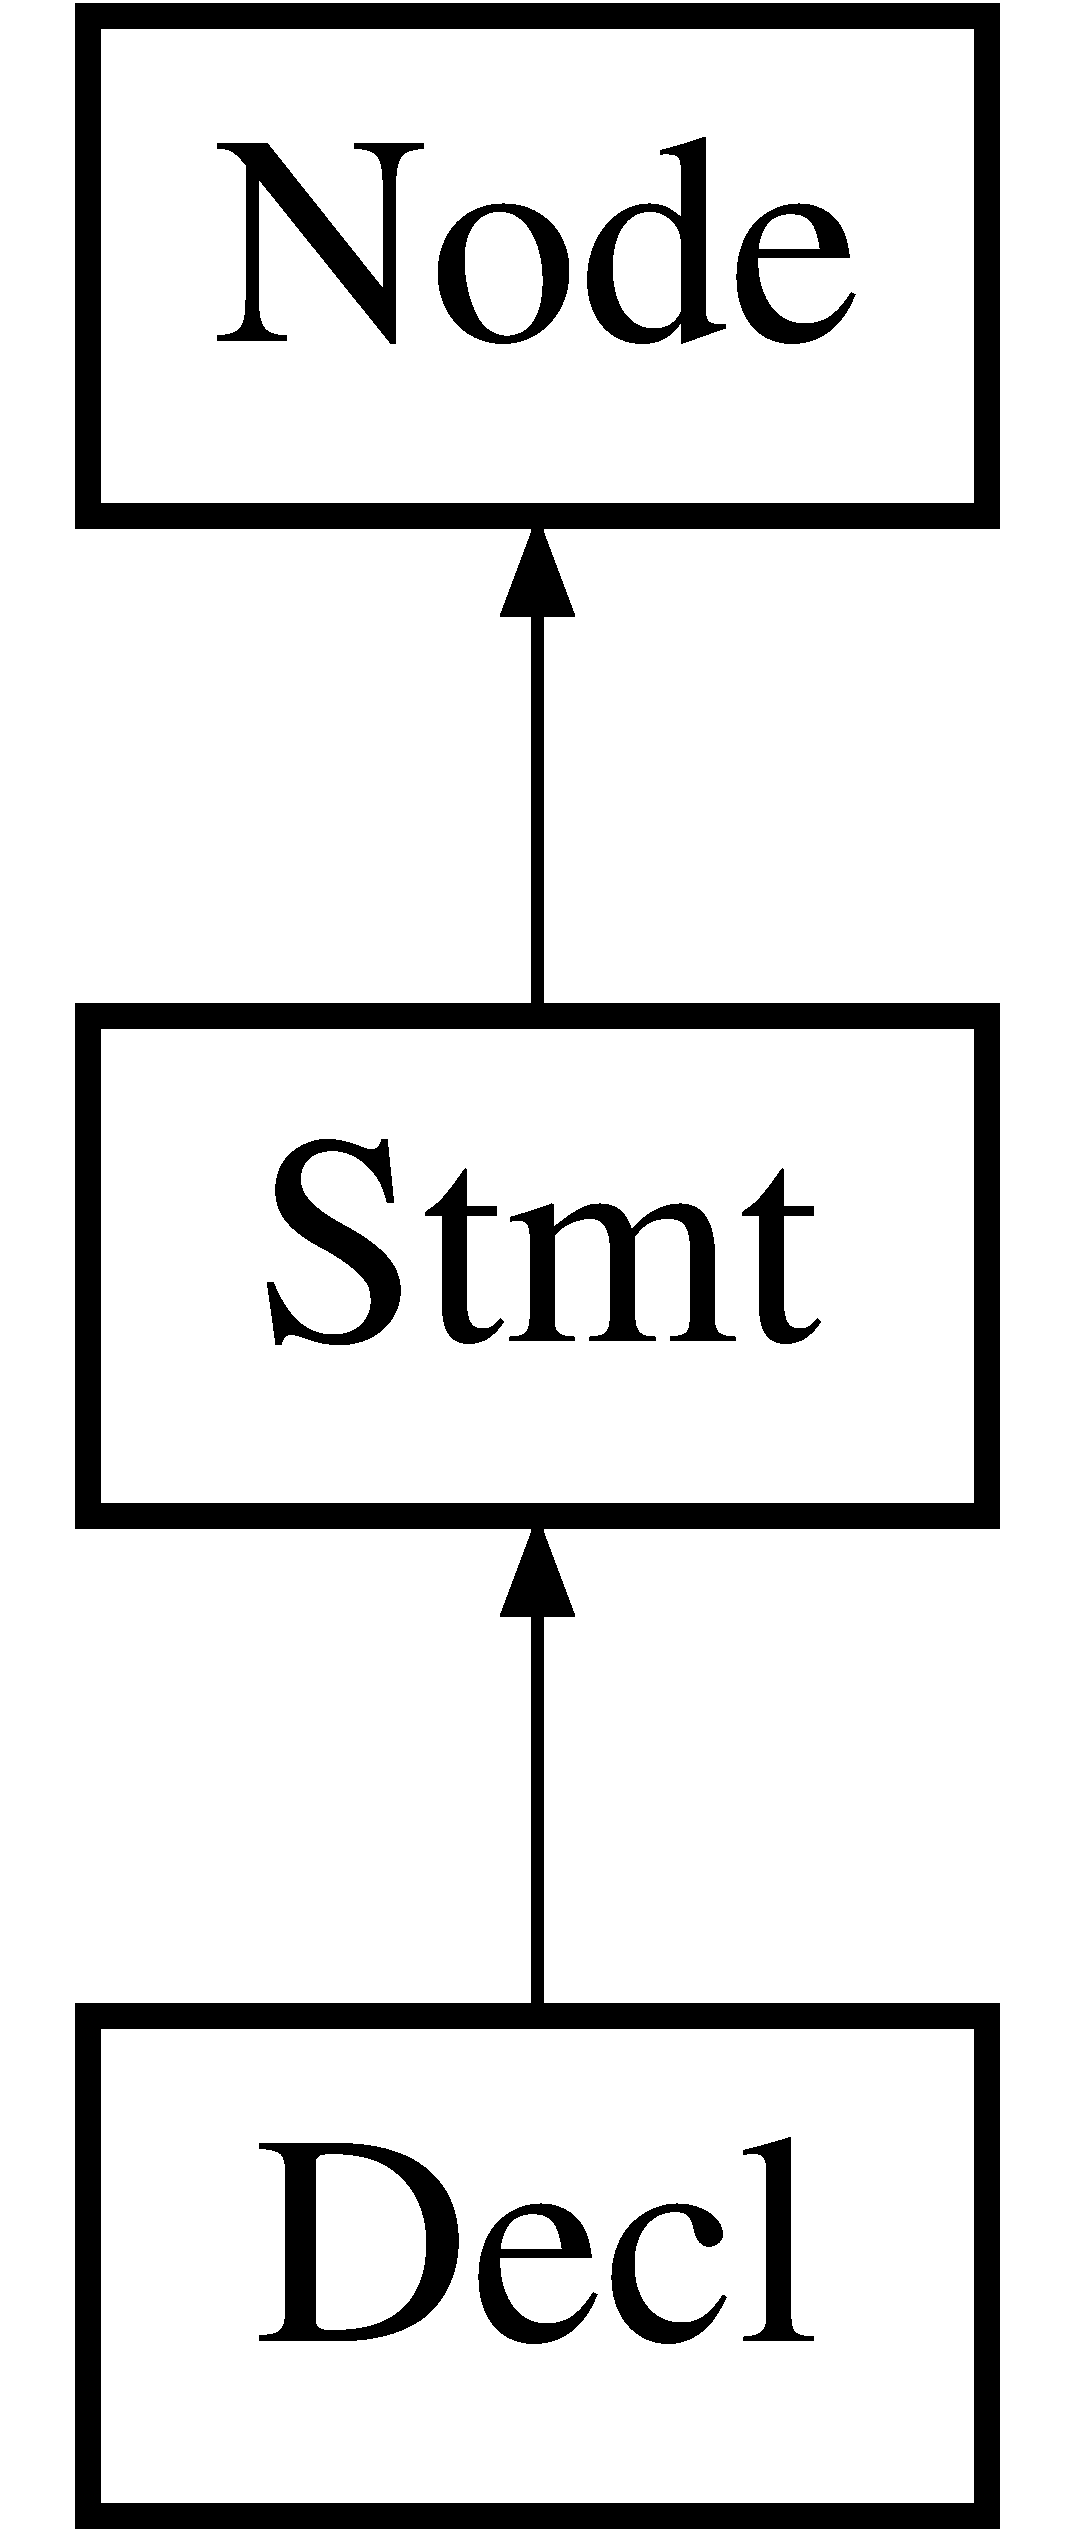
\includegraphics[height=3.000000cm]{class_decl}
\end{center}
\end{figure}
\subsection*{Public Member Functions}
\begin{DoxyCompactItemize}
\item 
\mbox{\Hypertarget{class_decl_ad6495a4245a45dcdcd05e239c8db4a8b}\label{class_decl_ad6495a4245a45dcdcd05e239c8db4a8b}} 
int \hyperlink{class_decl_ad6495a4245a45dcdcd05e239c8db4a8b}{execute} ()
\begin{DoxyCompactList}\small\item\em $<$ 执行变量声明 \end{DoxyCompactList}\item 
void \hyperlink{class_decl_a4c91db9c289b90f3045783f6bf53a688}{put} (\hyperlink{class_var}{Var} $\ast$, \hyperlink{class_expr}{Expr} $\ast$)
\item 
\mbox{\Hypertarget{class_decl_a356b82bee7d66a98c8fbb3547836b785}\label{class_decl_a356b82bee7d66a98c8fbb3547836b785}} 
\hyperlink{class_decl_a356b82bee7d66a98c8fbb3547836b785}{Decl} ()
\begin{DoxyCompactList}\small\item\em 初始化变量数组 \end{DoxyCompactList}\end{DoxyCompactItemize}
\subsection*{Protected Attributes}
\begin{DoxyCompactItemize}
\item 
\mbox{\Hypertarget{class_decl_a7e84697f4d13126d1234a49b68af7eeb}\label{class_decl_a7e84697f4d13126d1234a49b68af7eeb}} 
std\+::vector$<$ std\+::pair$<$ \hyperlink{class_var}{Var} $\ast$, \hyperlink{class_expr}{Expr} $\ast$ $>$ $>$ $\ast$ \hyperlink{class_decl_a7e84697f4d13126d1234a49b68af7eeb}{decls}
\begin{DoxyCompactList}\small\item\em 该语句中被声明的变量 \end{DoxyCompactList}\end{DoxyCompactItemize}
\subsection*{Additional Inherited Members}


\subsection{Detailed Description}
声明变量语句类 

\subsection{Member Function Documentation}
\mbox{\Hypertarget{class_decl_a4c91db9c289b90f3045783f6bf53a688}\label{class_decl_a4c91db9c289b90f3045783f6bf53a688}} 
\index{Decl@{Decl}!put@{put}}
\index{put@{put}!Decl@{Decl}}
\subsubsection{\texorpdfstring{put()}{put()}}
{\footnotesize\ttfamily void Decl\+::put (\begin{DoxyParamCaption}\item[{\hyperlink{class_var}{Var} $\ast$}]{var,  }\item[{\hyperlink{class_expr}{Expr} $\ast$}]{expr1 }\end{DoxyParamCaption})}

将变量与初始化用的表达式绑定 
\begin{DoxyParams}{Parameters}
{\em var} & \+: 被声明的变量 \\
\hline
{\em expr} & \+: 初始化表达式 \\
\hline
\end{DoxyParams}


The documentation for this class was generated from the following files\+:\begin{DoxyCompactItemize}
\item 
src/inter/stmt/Decl.\+h\item 
src/inter/stmt/Decl.\+cpp\end{DoxyCompactItemize}

\hypertarget{class_do_while}{}\section{Do\+While Class Reference}
\label{class_do_while}\index{Do\+While@{Do\+While}}


do-\/while循环语句类  




{\ttfamily \#include $<$Do\+While.\+h$>$}

Inheritance diagram for Do\+While\+:\begin{figure}[H]
\begin{center}
\leavevmode
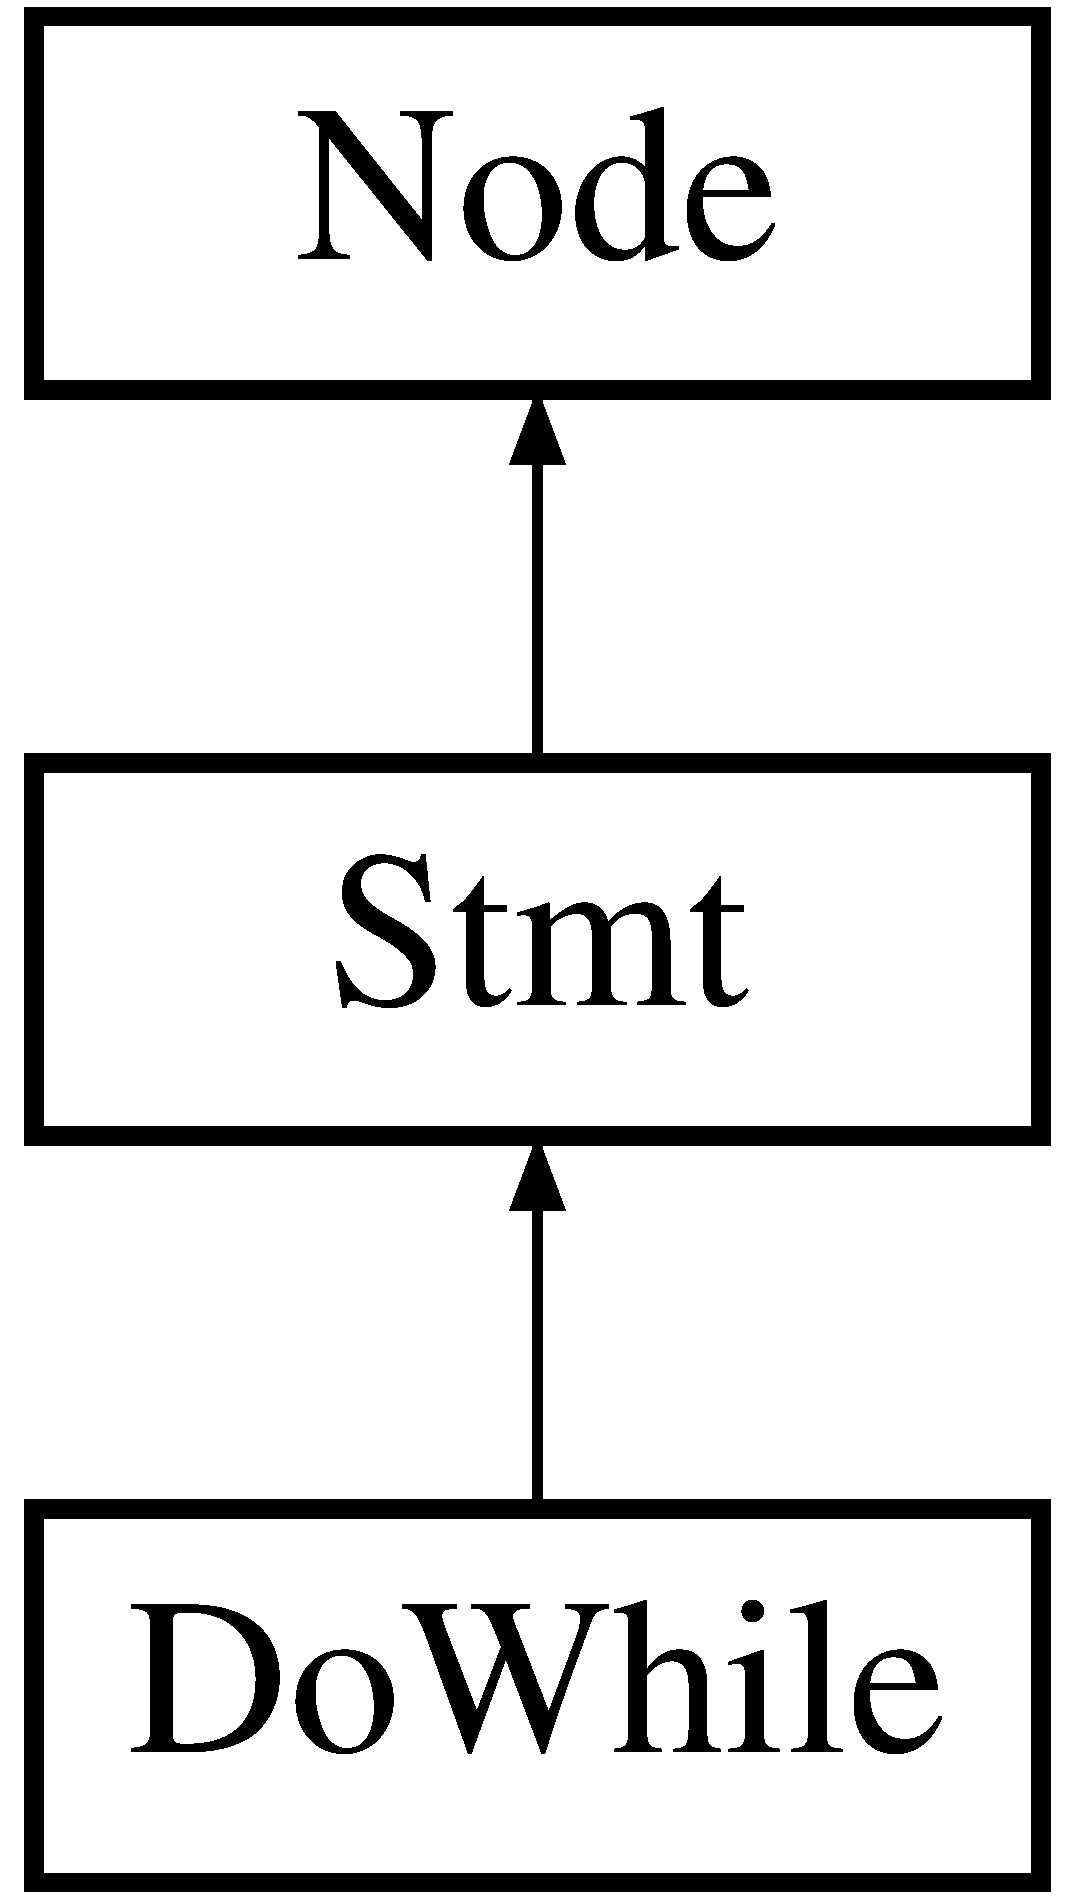
\includegraphics[height=3.000000cm]{class_do_while}
\end{center}
\end{figure}
\subsection*{Public Member Functions}
\begin{DoxyCompactItemize}
\item 
\mbox{\Hypertarget{class_do_while_adb6934e033f44c6b52b1079faf1d84cf}\label{class_do_while_adb6934e033f44c6b52b1079faf1d84cf}} 
int \hyperlink{class_do_while_adb6934e033f44c6b52b1079faf1d84cf}{execute} ()
\begin{DoxyCompactList}\small\item\em 执行do-\/while循环语句 \end{DoxyCompactList}\end{DoxyCompactItemize}
\subsection*{Public Attributes}
\begin{DoxyCompactItemize}
\item 
\mbox{\Hypertarget{class_do_while_a0aee68f104ddceeb30a4e061cf315e0f}\label{class_do_while_a0aee68f104ddceeb30a4e061cf315e0f}} 
\hyperlink{class_stmt}{Stmt} $\ast$ \hyperlink{class_do_while_a0aee68f104ddceeb30a4e061cf315e0f}{stmt}
\begin{DoxyCompactList}\small\item\em 循环体语句 \end{DoxyCompactList}\item 
\hyperlink{class_expr}{Expr} $\ast$ \hyperlink{class_do_while_a55d5ffb9c6bee10f8375f028705e4901}{expr}
\end{DoxyCompactItemize}
\subsection*{Additional Inherited Members}


\subsection{Detailed Description}
do-\/while循环语句类 

\subsection{Member Data Documentation}
\mbox{\Hypertarget{class_do_while_a55d5ffb9c6bee10f8375f028705e4901}\label{class_do_while_a55d5ffb9c6bee10f8375f028705e4901}} 
\index{Do\+While@{Do\+While}!expr@{expr}}
\index{expr@{expr}!Do\+While@{Do\+While}}
\subsubsection{\texorpdfstring{expr}{expr}}
{\footnotesize\ttfamily \hyperlink{class_expr}{Expr}$\ast$ Do\+While\+::expr}

条件表达式 

The documentation for this class was generated from the following files\+:\begin{DoxyCompactItemize}
\item 
src/inter/stmt/Do\+While.\+h\item 
src/inter/stmt/Do\+While.\+cpp\end{DoxyCompactItemize}

\hypertarget{class_duplicate_decl}{}\section{Duplicate\+Decl Class Reference}
\label{class_duplicate_decl}\index{Duplicate\+Decl@{Duplicate\+Decl}}


Duplicate\+Decl类  




{\ttfamily \#include $<$Duplicate\+Decl.\+h$>$}

Inheritance diagram for Duplicate\+Decl\+:\begin{figure}[H]
\begin{center}
\leavevmode
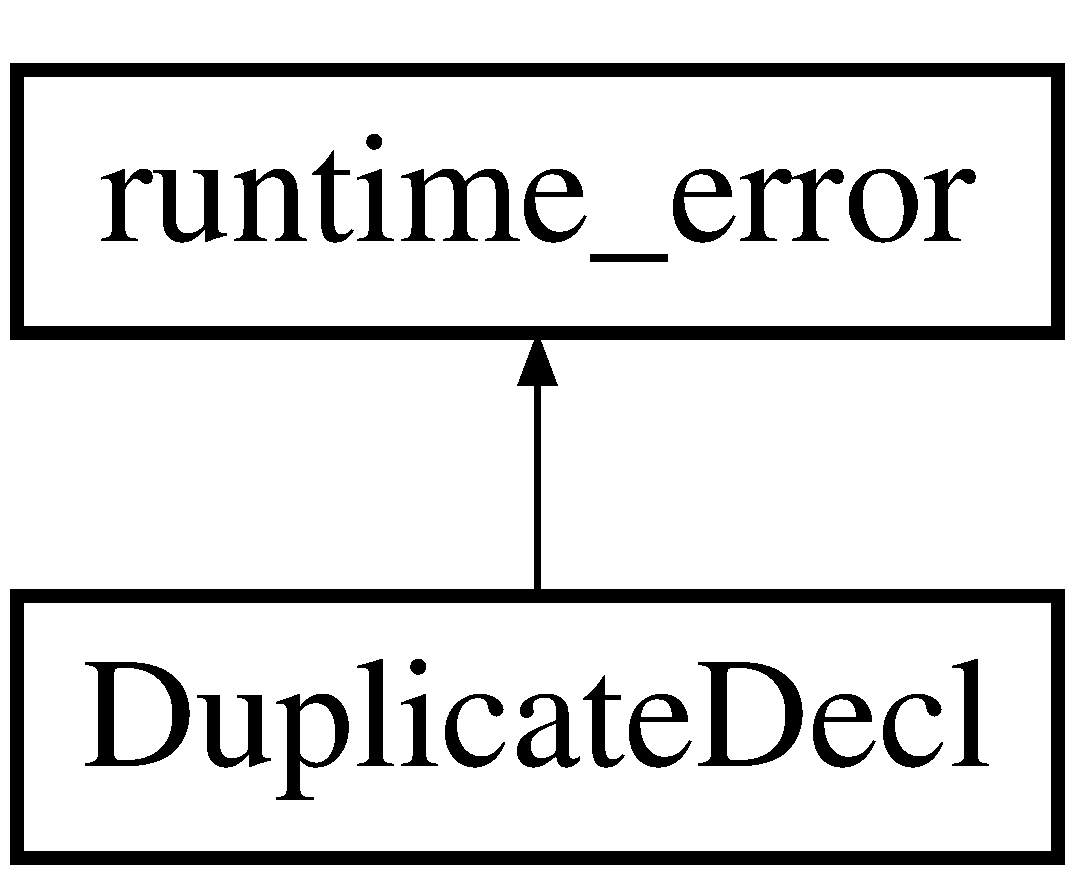
\includegraphics[height=2.000000cm]{class_duplicate_decl}
\end{center}
\end{figure}
\subsection*{Public Member Functions}
\begin{DoxyCompactItemize}
\item 
\mbox{\Hypertarget{class_duplicate_decl_a101a07d46a713363621da69f46a711b3}\label{class_duplicate_decl_a101a07d46a713363621da69f46a711b3}} 
{\bfseries Duplicate\+Decl} (std\+::string)
\end{DoxyCompactItemize}


\subsection{Detailed Description}
Duplicate\+Decl类 

重复定义变量错误~\newline
若一个变量在一个同一个作用域中被声明了两次将抛出此错误 

The documentation for this class was generated from the following files\+:\begin{DoxyCompactItemize}
\item 
src/inter/error/Duplicate\+Decl.\+h\item 
src/inter/error/Duplicate\+Decl.\+cpp\end{DoxyCompactItemize}

\hypertarget{class_env}{}\section{Env Class Reference}
\label{class_env}\index{Env@{Env}}


变量环境类  




{\ttfamily \#include $<$Env.\+h$>$}

\subsection*{Public Member Functions}
\begin{DoxyCompactItemize}
\item 
\hyperlink{class_env_ab9d20c5b47453e30038f156cc5e25c0f}{Env} (\hyperlink{class_env}{Env} $\ast$)
\begin{DoxyCompactList}\small\item\em 初始化当前环境 \end{DoxyCompactList}\item 
\mbox{\Hypertarget{class_env_a4648c2b83fea7e757ccb4ab519ffc9a0}\label{class_env_a4648c2b83fea7e757ccb4ab519ffc9a0}} 
void \hyperlink{class_env_a4648c2b83fea7e757ccb4ab519ffc9a0}{put} (std\+::string, \hyperlink{class_id}{Id})
\begin{DoxyCompactList}\small\item\em 向环境中添加新的变量 \end{DoxyCompactList}\item 
\hyperlink{class_id}{Id} $\ast$ \hyperlink{class_env_a59bbdcdb7af396f6fb6cbff2f828e62b}{get} (std\+::string)
\begin{DoxyCompactList}\small\item\em 获取变量 \end{DoxyCompactList}\item 
void \hyperlink{class_env_a398c166330482abb7e38c546bc3974cf}{print\+Current\+Var} ()
\begin{DoxyCompactList}\small\item\em 输出当前环境中的所有变量 \end{DoxyCompactList}\item 
void \hyperlink{class_env_a8ba6704ef2039c2329569efc99f1e087}{print\+All\+Var} ()
\begin{DoxyCompactList}\small\item\em 输出所有的环境中的变量 \end{DoxyCompactList}\end{DoxyCompactItemize}
\subsection*{Protected Member Functions}
\begin{DoxyCompactItemize}
\item 
\hyperlink{class_id}{Id} $\ast$ \hyperlink{class_env_aca71253ff9d30153d0834a47cd35a351}{\+\_\+get} (std\+::string)
\begin{DoxyCompactList}\small\item\em 获取当前变量 \end{DoxyCompactList}\end{DoxyCompactItemize}
\subsection*{Protected Attributes}
\begin{DoxyCompactItemize}
\item 
\hyperlink{class_env}{Env} $\ast$ \hyperlink{class_env_a79a41e9166e949e4c1320ffe3750cb29}{prev}
\end{DoxyCompactItemize}
\subsection*{Private Attributes}
\begin{DoxyCompactItemize}
\item 
\mbox{\Hypertarget{class_env_ab93397b135a614cb1c7e6057a00a8d85}\label{class_env_ab93397b135a614cb1c7e6057a00a8d85}} 
std\+::map$<$ std\+::string, \hyperlink{class_id}{Id} $>$ \hyperlink{class_env_ab93397b135a614cb1c7e6057a00a8d85}{table}
\begin{DoxyCompactList}\small\item\em 当前环境的环境变量表 \end{DoxyCompactList}\end{DoxyCompactItemize}


\subsection{Detailed Description}
变量环境类 

\subsection{Constructor \& Destructor Documentation}
\mbox{\Hypertarget{class_env_ab9d20c5b47453e30038f156cc5e25c0f}\label{class_env_ab9d20c5b47453e30038f156cc5e25c0f}} 
\index{Env@{Env}!Env@{Env}}
\index{Env@{Env}!Env@{Env}}
\subsubsection{\texorpdfstring{Env()}{Env()}}
{\footnotesize\ttfamily Env\+::\+Env (\begin{DoxyParamCaption}\item[{\hyperlink{class_env}{Env} $\ast$}]{n }\end{DoxyParamCaption})}



初始化当前环境 


\begin{DoxyParams}{Parameters}
{\em env} & \+: 上一层环境的指针 \\
\hline
\end{DoxyParams}


\subsection{Member Function Documentation}
\mbox{\Hypertarget{class_env_aca71253ff9d30153d0834a47cd35a351}\label{class_env_aca71253ff9d30153d0834a47cd35a351}} 
\index{Env@{Env}!\+\_\+get@{\+\_\+get}}
\index{\+\_\+get@{\+\_\+get}!Env@{Env}}
\subsubsection{\texorpdfstring{\+\_\+get()}{\_get()}}
{\footnotesize\ttfamily \hyperlink{class_id}{Id} $\ast$ Env\+::\+\_\+get (\begin{DoxyParamCaption}\item[{std\+::string}]{word }\end{DoxyParamCaption})\hspace{0.3cm}{\ttfamily [protected]}}



获取当前变量 

在当前表中查找 \mbox{\Hypertarget{class_env_a59bbdcdb7af396f6fb6cbff2f828e62b}\label{class_env_a59bbdcdb7af396f6fb6cbff2f828e62b}} 
\index{Env@{Env}!get@{get}}
\index{get@{get}!Env@{Env}}
\subsubsection{\texorpdfstring{get()}{get()}}
{\footnotesize\ttfamily \hyperlink{class_id}{Id} $\ast$ Env\+::get (\begin{DoxyParamCaption}\item[{std\+::string}]{word }\end{DoxyParamCaption})}



获取变量 

在表链中查找 迭代实现 \mbox{\Hypertarget{class_env_a8ba6704ef2039c2329569efc99f1e087}\label{class_env_a8ba6704ef2039c2329569efc99f1e087}} 
\index{Env@{Env}!print\+All\+Var@{print\+All\+Var}}
\index{print\+All\+Var@{print\+All\+Var}!Env@{Env}}
\subsubsection{\texorpdfstring{print\+All\+Var()}{printAllVar()}}
{\footnotesize\ttfamily void Env\+::print\+All\+Var (\begin{DoxyParamCaption}{ }\end{DoxyParamCaption})}



输出所有的环境中的变量 

打印作用域链所有变量 调试使用 \mbox{\Hypertarget{class_env_a398c166330482abb7e38c546bc3974cf}\label{class_env_a398c166330482abb7e38c546bc3974cf}} 
\index{Env@{Env}!print\+Current\+Var@{print\+Current\+Var}}
\index{print\+Current\+Var@{print\+Current\+Var}!Env@{Env}}
\subsubsection{\texorpdfstring{print\+Current\+Var()}{printCurrentVar()}}
{\footnotesize\ttfamily void Env\+::print\+Current\+Var (\begin{DoxyParamCaption}{ }\end{DoxyParamCaption})}



输出当前环境中的所有变量 

打印当前block作用域变量 调试使用 

\subsection{Member Data Documentation}
\mbox{\Hypertarget{class_env_a79a41e9166e949e4c1320ffe3750cb29}\label{class_env_a79a41e9166e949e4c1320ffe3750cb29}} 
\index{Env@{Env}!prev@{prev}}
\index{prev@{prev}!Env@{Env}}
\subsubsection{\texorpdfstring{prev}{prev}}
{\footnotesize\ttfamily \hyperlink{class_env}{Env}$\ast$ Env\+::prev\hspace{0.3cm}{\ttfamily [protected]}}

上一层环境变量的指针 

The documentation for this class was generated from the following files\+:\begin{DoxyCompactItemize}
\item 
src/symbols/Env.\+h\item 
src/symbols/Env.\+cpp\end{DoxyCompactItemize}

\hypertarget{class_equality}{}\section{Equality类 参考}
\label{class_equality}\index{Equality@{Equality}}


等于不等于表达式类  




{\ttfamily \#include $<$Equality.\+h$>$}

类 Equality 继承关系图\+:\begin{figure}[H]
\begin{center}
\leavevmode
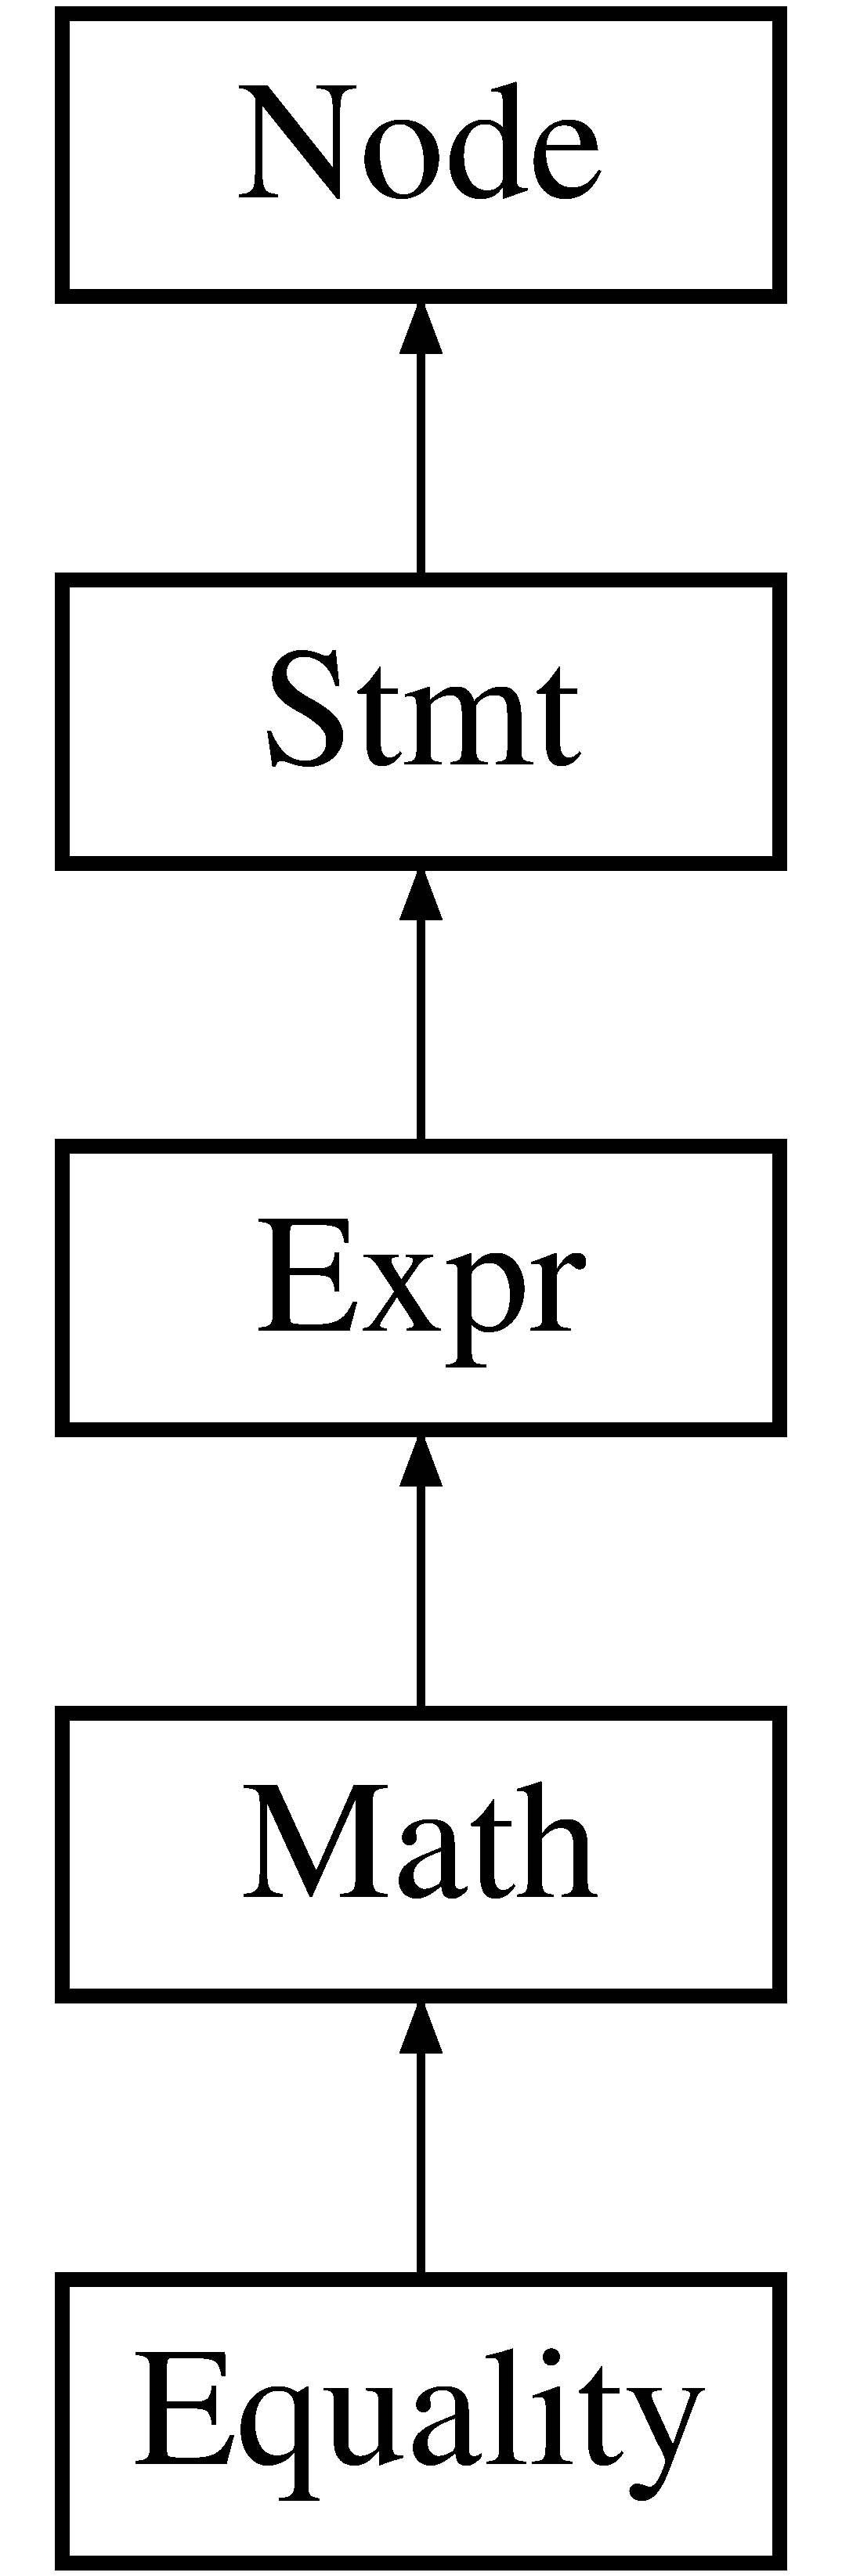
\includegraphics[height=5.000000cm]{class_equality}
\end{center}
\end{figure}
\subsection*{Public 成员函数}
\begin{DoxyCompactItemize}
\item 
\hyperlink{class_equality_afe12b1491ae42b80d41a8355bfe3197c}{Equality} (\hyperlink{class_token}{Token} $\ast$token, \hyperlink{class_expr}{Expr} $\ast$expr1, \hyperlink{class_expr}{Expr} $\ast$expr2)
\item 
int \hyperlink{class_equality_a0255c33af70613b006b03a329ed329ff}{execute} ()
\end{DoxyCompactItemize}
\subsection*{额外继承的成员函数}


\subsection{详细描述}
等于不等于表达式类 

\subsection{构造及析构函数说明}
\index{Equality@{Equality}!Equality@{Equality}}
\index{Equality@{Equality}!Equality@{Equality}}
\subsubsection[{\texorpdfstring{Equality(\+Token $\ast$token, Expr $\ast$expr1, Expr $\ast$expr2)}{Equality(Token *token, Expr *expr1, Expr *expr2)}}]{\setlength{\rightskip}{0pt plus 5cm}Equality\+::\+Equality (
\begin{DoxyParamCaption}
\item[{{\bf Token} $\ast$}]{token, }
\item[{{\bf Expr} $\ast$}]{expr1, }
\item[{{\bf Expr} $\ast$}]{expr2}
\end{DoxyParamCaption}
)}\hypertarget{class_equality_afe12b1491ae42b80d41a8355bfe3197c}{}\label{class_equality_afe12b1491ae42b80d41a8355bfe3197c}

\begin{DoxyParams}{参数}
{\em token} & \+: 标识运算符的 token \\
\hline
{\em expr1} & \+: 左表达式 \\
\hline
{\em expr2} & \+: 右表达式 \\
\hline
\end{DoxyParams}


\subsection{成员函数说明}
\index{Equality@{Equality}!execute@{execute}}
\index{execute@{execute}!Equality@{Equality}}
\subsubsection[{\texorpdfstring{execute()}{execute()}}]{\setlength{\rightskip}{0pt plus 5cm}int Equality\+::execute (
\begin{DoxyParamCaption}
{}
\end{DoxyParamCaption}
)\hspace{0.3cm}{\ttfamily [virtual]}}\hypertarget{class_equality_a0255c33af70613b006b03a329ed329ff}{}\label{class_equality_a0255c33af70613b006b03a329ed329ff}
\begin{DoxyReturn}{返回}
执行后的值 
\end{DoxyReturn}


重载 \hyperlink{class_expr_aff6a2e6eaa460e2a3db28ebdab089b51}{Expr} .



该类的文档由以下文件生成\+:\begin{DoxyCompactItemize}
\item 
src/inter/stmt/expr/Equality.\+h\item 
src/inter/stmt/expr/Equality.\+cpp\end{DoxyCompactItemize}

\hypertarget{class_expr}{}\section{Expr Class Reference}
\label{class_expr}\index{Expr@{Expr}}


运算表达式类  




{\ttfamily \#include $<$Expr.\+h$>$}

Inheritance diagram for Expr\+:\begin{figure}[H]
\begin{center}
\leavevmode
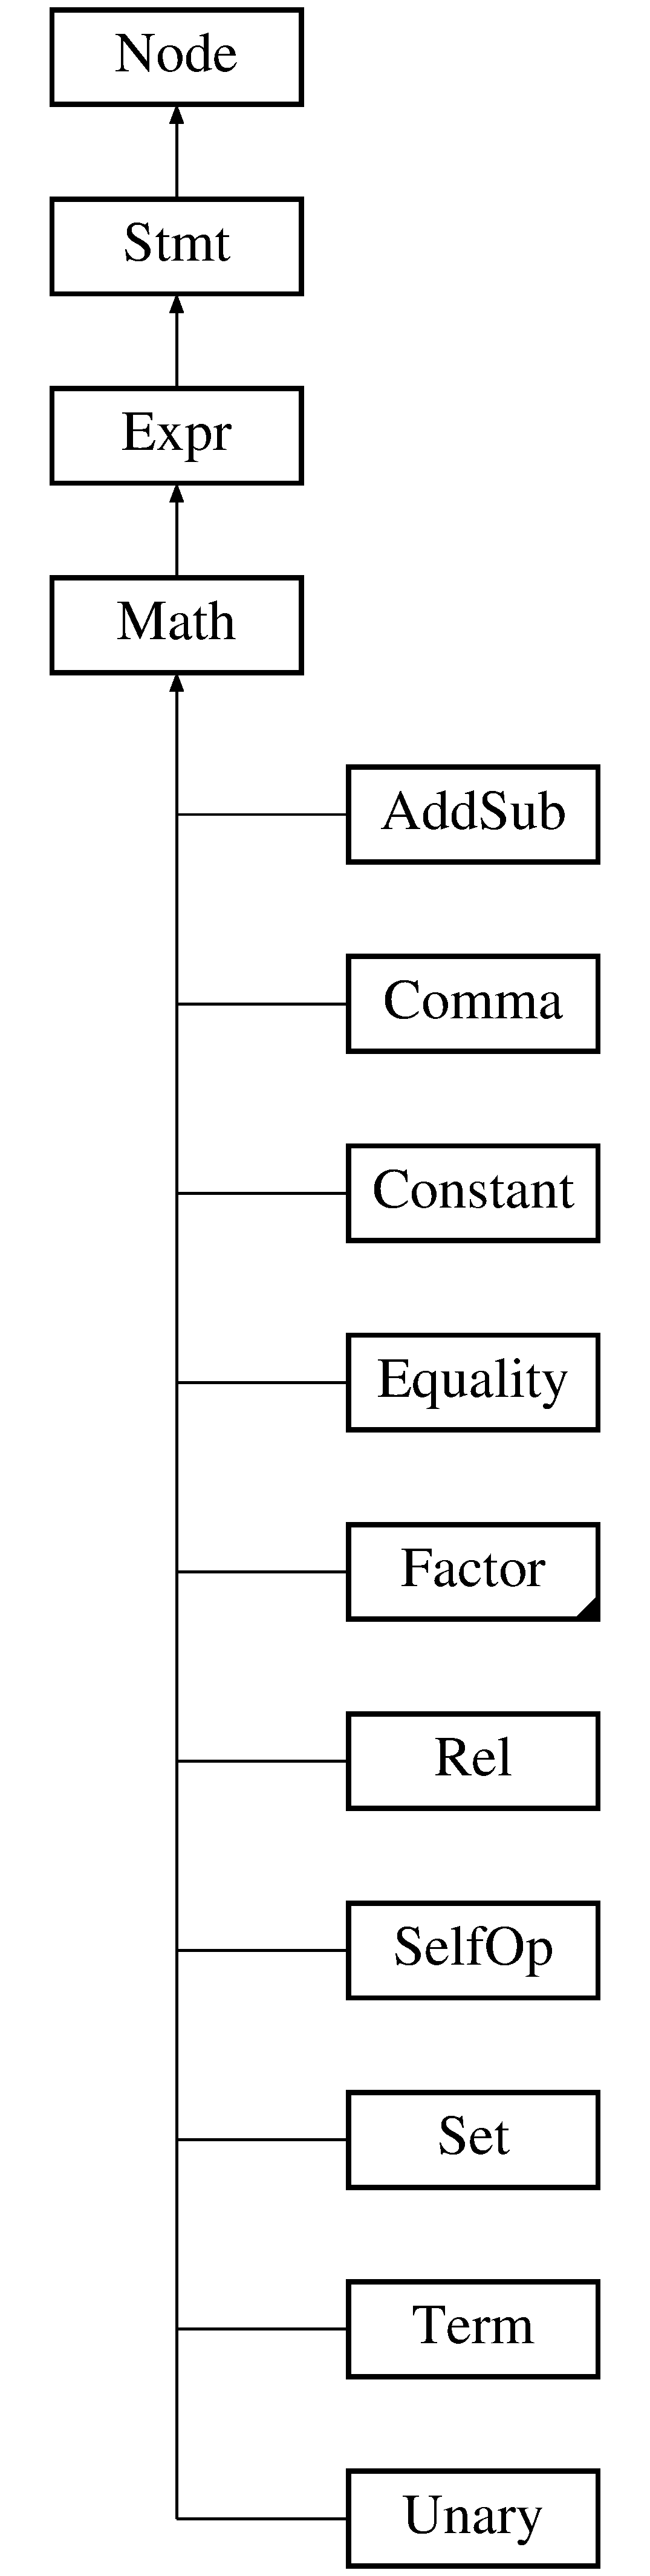
\includegraphics[height=12.000000cm]{class_expr}
\end{center}
\end{figure}
\subsection*{Public Member Functions}
\begin{DoxyCompactItemize}
\item 
\hyperlink{class_expr_a5a045d68e601c2e782e1958d55a07400}{Expr} (\hyperlink{class_token}{Token} $\ast$)
\item 
virtual int \hyperlink{class_expr_aff6a2e6eaa460e2a3db28ebdab089b51}{execute} ()
\item 
\mbox{\Hypertarget{class_expr_add2b30644dd850c4bfa2d619d20d8c09}\label{class_expr_add2b30644dd850c4bfa2d619d20d8c09}} 
virtual bool {\bfseries is\+Var} ()
\end{DoxyCompactItemize}
\subsection*{Public Attributes}
\begin{DoxyCompactItemize}
\item 
\hyperlink{class_token}{Token} $\ast$ \hyperlink{class_expr_a5fd7721b7843686e3ec7e63fddf95644}{op}
\end{DoxyCompactItemize}
\subsection*{Additional Inherited Members}


\subsection{Detailed Description}
运算表达式类 

\subsection{Constructor \& Destructor Documentation}
\mbox{\Hypertarget{class_expr_a5a045d68e601c2e782e1958d55a07400}\label{class_expr_a5a045d68e601c2e782e1958d55a07400}} 
\index{Expr@{Expr}!Expr@{Expr}}
\index{Expr@{Expr}!Expr@{Expr}}
\subsubsection{\texorpdfstring{Expr()}{Expr()}}
{\footnotesize\ttfamily Expr\+::\+Expr (\begin{DoxyParamCaption}\item[{\hyperlink{class_token}{Token} $\ast$}]{token }\end{DoxyParamCaption})}


\begin{DoxyParams}{Parameters}
{\em token} & \+: 标识运算因子类型的 token \\
\hline
\end{DoxyParams}


\subsection{Member Function Documentation}
\mbox{\Hypertarget{class_expr_aff6a2e6eaa460e2a3db28ebdab089b51}\label{class_expr_aff6a2e6eaa460e2a3db28ebdab089b51}} 
\index{Expr@{Expr}!execute@{execute}}
\index{execute@{execute}!Expr@{Expr}}
\subsubsection{\texorpdfstring{execute()}{execute()}}
{\footnotesize\ttfamily int Expr\+::execute (\begin{DoxyParamCaption}{ }\end{DoxyParamCaption})\hspace{0.3cm}{\ttfamily [virtual]}}

\begin{DoxyReturn}{Returns}
执行后的值 
\end{DoxyReturn}


Reimplemented from \hyperlink{class_stmt_abdc3261770c3c5bd3ce5b3ba6eedfaa4}{Stmt}.



Reimplemented in \hyperlink{class_var_a9dc96e803f7b0f9aa519c2c0e0a6bd8f}{Var}, \hyperlink{class_set_a7776ba36f3af8b09772b36927beb5f5c}{Set}, \hyperlink{class_unary_af42edff1ee4718a9afeb7127e41af758}{Unary}, \hyperlink{class_comma_aab9ca2bb70a10abd2fb263de745f843a}{Comma}, \hyperlink{class_equality_a0255c33af70613b006b03a329ed329ff}{Equality}, \hyperlink{class_term_ac2d20115da73f9425e5d390856a211a1}{Term}, \hyperlink{class_rel_a82b2f3b75a2b9e81631f2659d42a36d1}{Rel}, \hyperlink{class_self_op_ab452bcad1cd4f1286813b1f737583818}{Self\+Op}, \hyperlink{class_add_sub_a73c0513a31a5400fdfc79ce877a1c3b9}{Add\+Sub}, \hyperlink{class_id_ae43a9ffecbbc0ac4fd041b8e8e3c3de0}{Id}, and \hyperlink{class_constant_ab5c55607bcff5ce70131a588b6bdbed7}{Constant}.



\subsection{Member Data Documentation}
\mbox{\Hypertarget{class_expr_a5fd7721b7843686e3ec7e63fddf95644}\label{class_expr_a5fd7721b7843686e3ec7e63fddf95644}} 
\index{Expr@{Expr}!op@{op}}
\index{op@{op}!Expr@{Expr}}
\subsubsection{\texorpdfstring{op}{op}}
{\footnotesize\ttfamily \hyperlink{class_token}{Token}$\ast$ Expr\+::op}

标识操作的 token 

The documentation for this class was generated from the following files\+:\begin{DoxyCompactItemize}
\item 
src/inter/stmt/expr/Expr.\+h\item 
src/inter/stmt/expr/Expr.\+cpp\end{DoxyCompactItemize}

\hypertarget{class_factor}{}\section{Factor Class Reference}
\label{class_factor}\index{Factor@{Factor}}


运算因子类  




{\ttfamily \#include $<$Factor.\+h$>$}

Inheritance diagram for Factor\+:\begin{figure}[H]
\begin{center}
\leavevmode
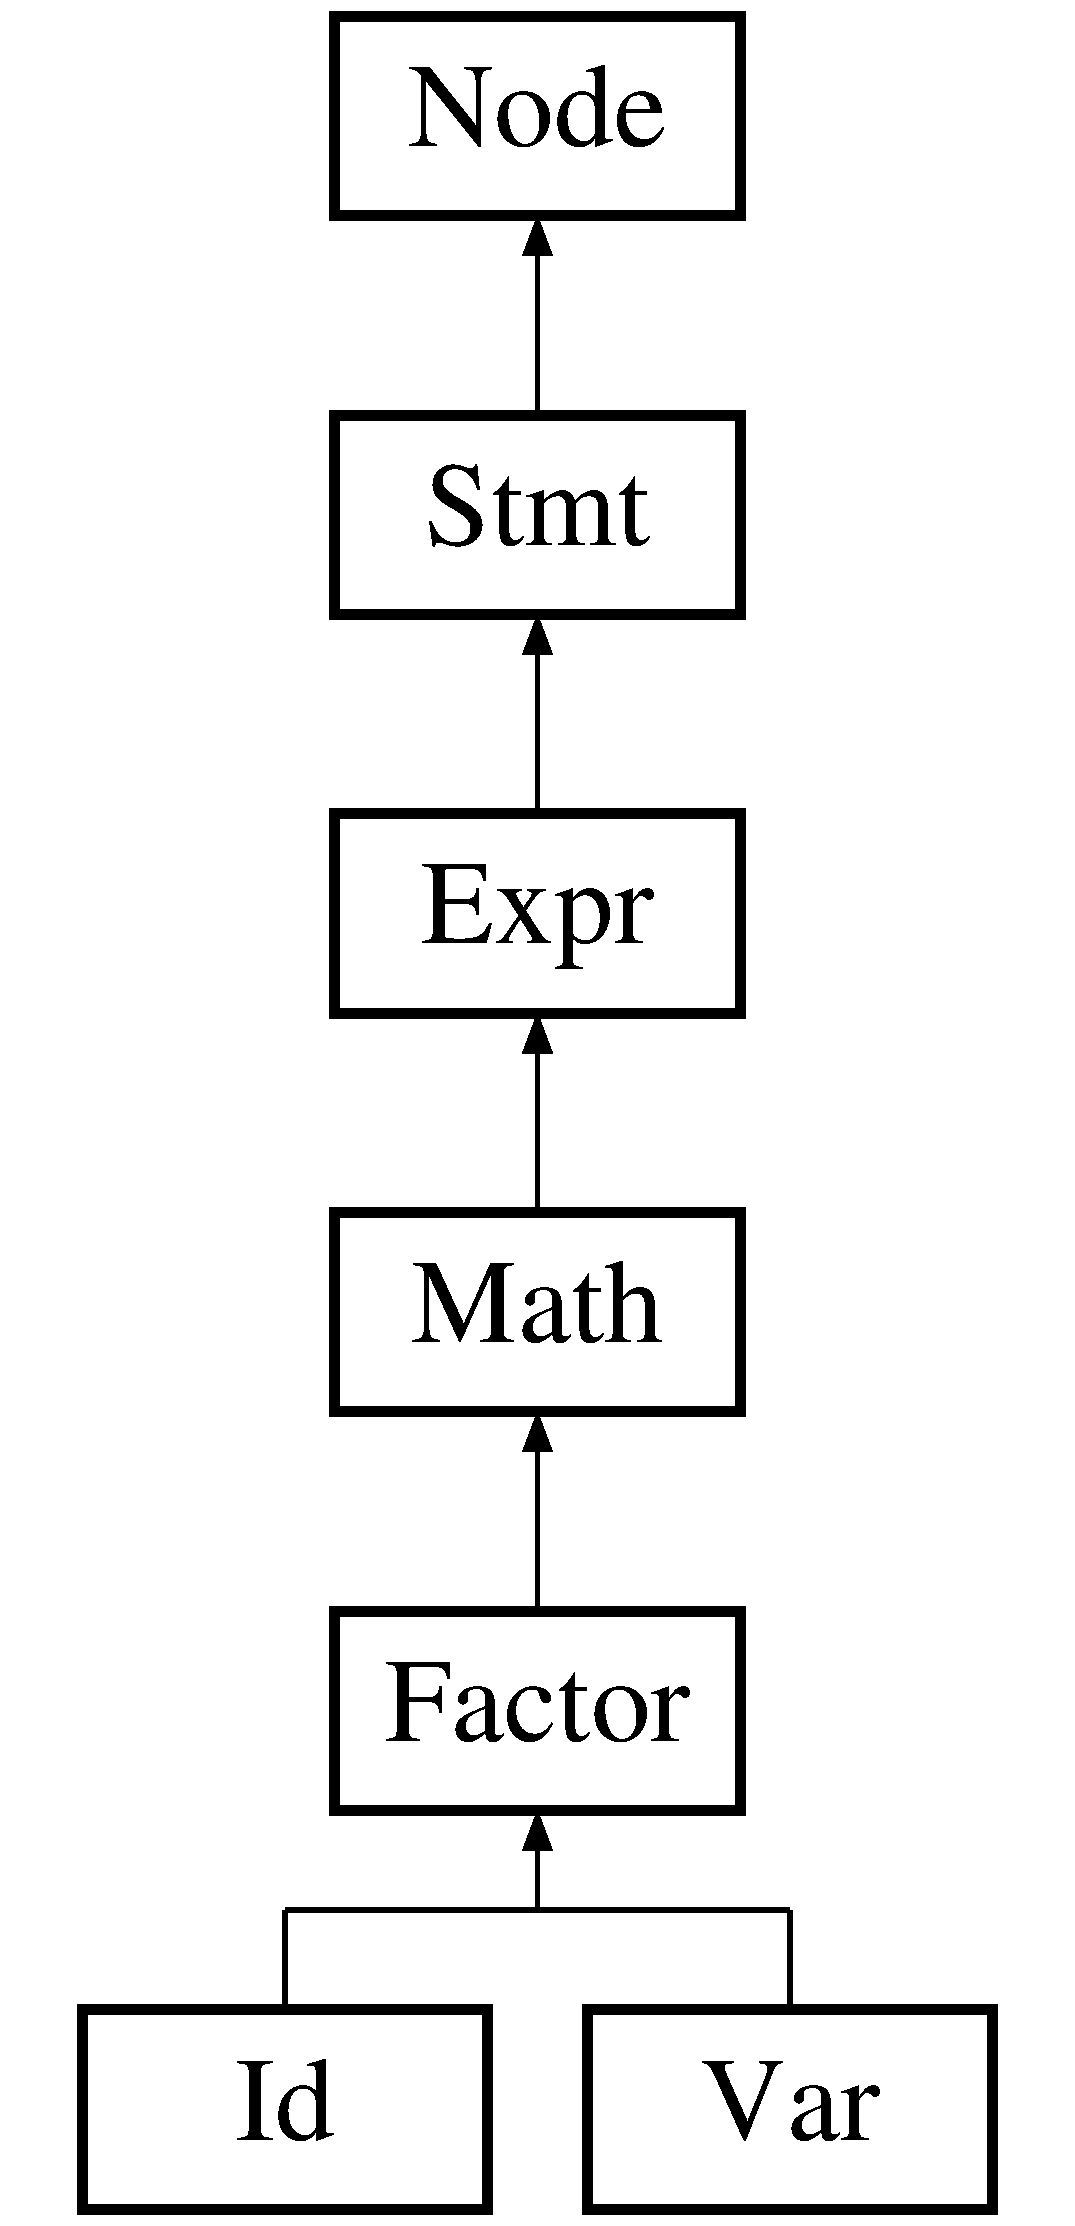
\includegraphics[height=6.000000cm]{class_factor}
\end{center}
\end{figure}
\subsection*{Public Member Functions}
\begin{DoxyCompactItemize}
\item 
\hyperlink{class_factor_af17f55c01064dcb353c47243931d095a}{Factor} (\hyperlink{class_token}{Token} $\ast$)
\end{DoxyCompactItemize}
\subsection*{Public Attributes}
\begin{DoxyCompactItemize}
\item 
\hyperlink{class_token}{Token} $\ast$ \hyperlink{class_factor_ab2c56fe952c0e3dad6006950e166495b}{token}
\end{DoxyCompactItemize}
\subsection*{Additional Inherited Members}


\subsection{Detailed Description}
运算因子类 

\subsection{Constructor \& Destructor Documentation}
\mbox{\Hypertarget{class_factor_af17f55c01064dcb353c47243931d095a}\label{class_factor_af17f55c01064dcb353c47243931d095a}} 
\index{Factor@{Factor}!Factor@{Factor}}
\index{Factor@{Factor}!Factor@{Factor}}
\subsubsection{\texorpdfstring{Factor()}{Factor()}}
{\footnotesize\ttfamily Factor\+::\+Factor (\begin{DoxyParamCaption}\item[{\hyperlink{class_token}{Token} $\ast$}]{token1 }\end{DoxyParamCaption})}


\begin{DoxyParams}{Parameters}
{\em token} & \+: 标识运算因子类型的 token \\
\hline
\end{DoxyParams}


\subsection{Member Data Documentation}
\mbox{\Hypertarget{class_factor_ab2c56fe952c0e3dad6006950e166495b}\label{class_factor_ab2c56fe952c0e3dad6006950e166495b}} 
\index{Factor@{Factor}!token@{token}}
\index{token@{token}!Factor@{Factor}}
\subsubsection{\texorpdfstring{token}{token}}
{\footnotesize\ttfamily \hyperlink{class_token}{Token}$\ast$ Factor\+::token}

标识运算因子类型的 token 

The documentation for this class was generated from the following files\+:\begin{DoxyCompactItemize}
\item 
src/inter/stmt/expr/\hyperlink{_factor_8h}{Factor.\+h}\item 
src/inter/stmt/expr/\hyperlink{_factor_8cpp}{Factor.\+cpp}\end{DoxyCompactItemize}

\hypertarget{class_for}{}\section{For类 参考}
\label{class_for}\index{For@{For}}


for循环语句类  




{\ttfamily \#include $<$For.\+h$>$}

类 For 继承关系图\+:\begin{figure}[H]
\begin{center}
\leavevmode
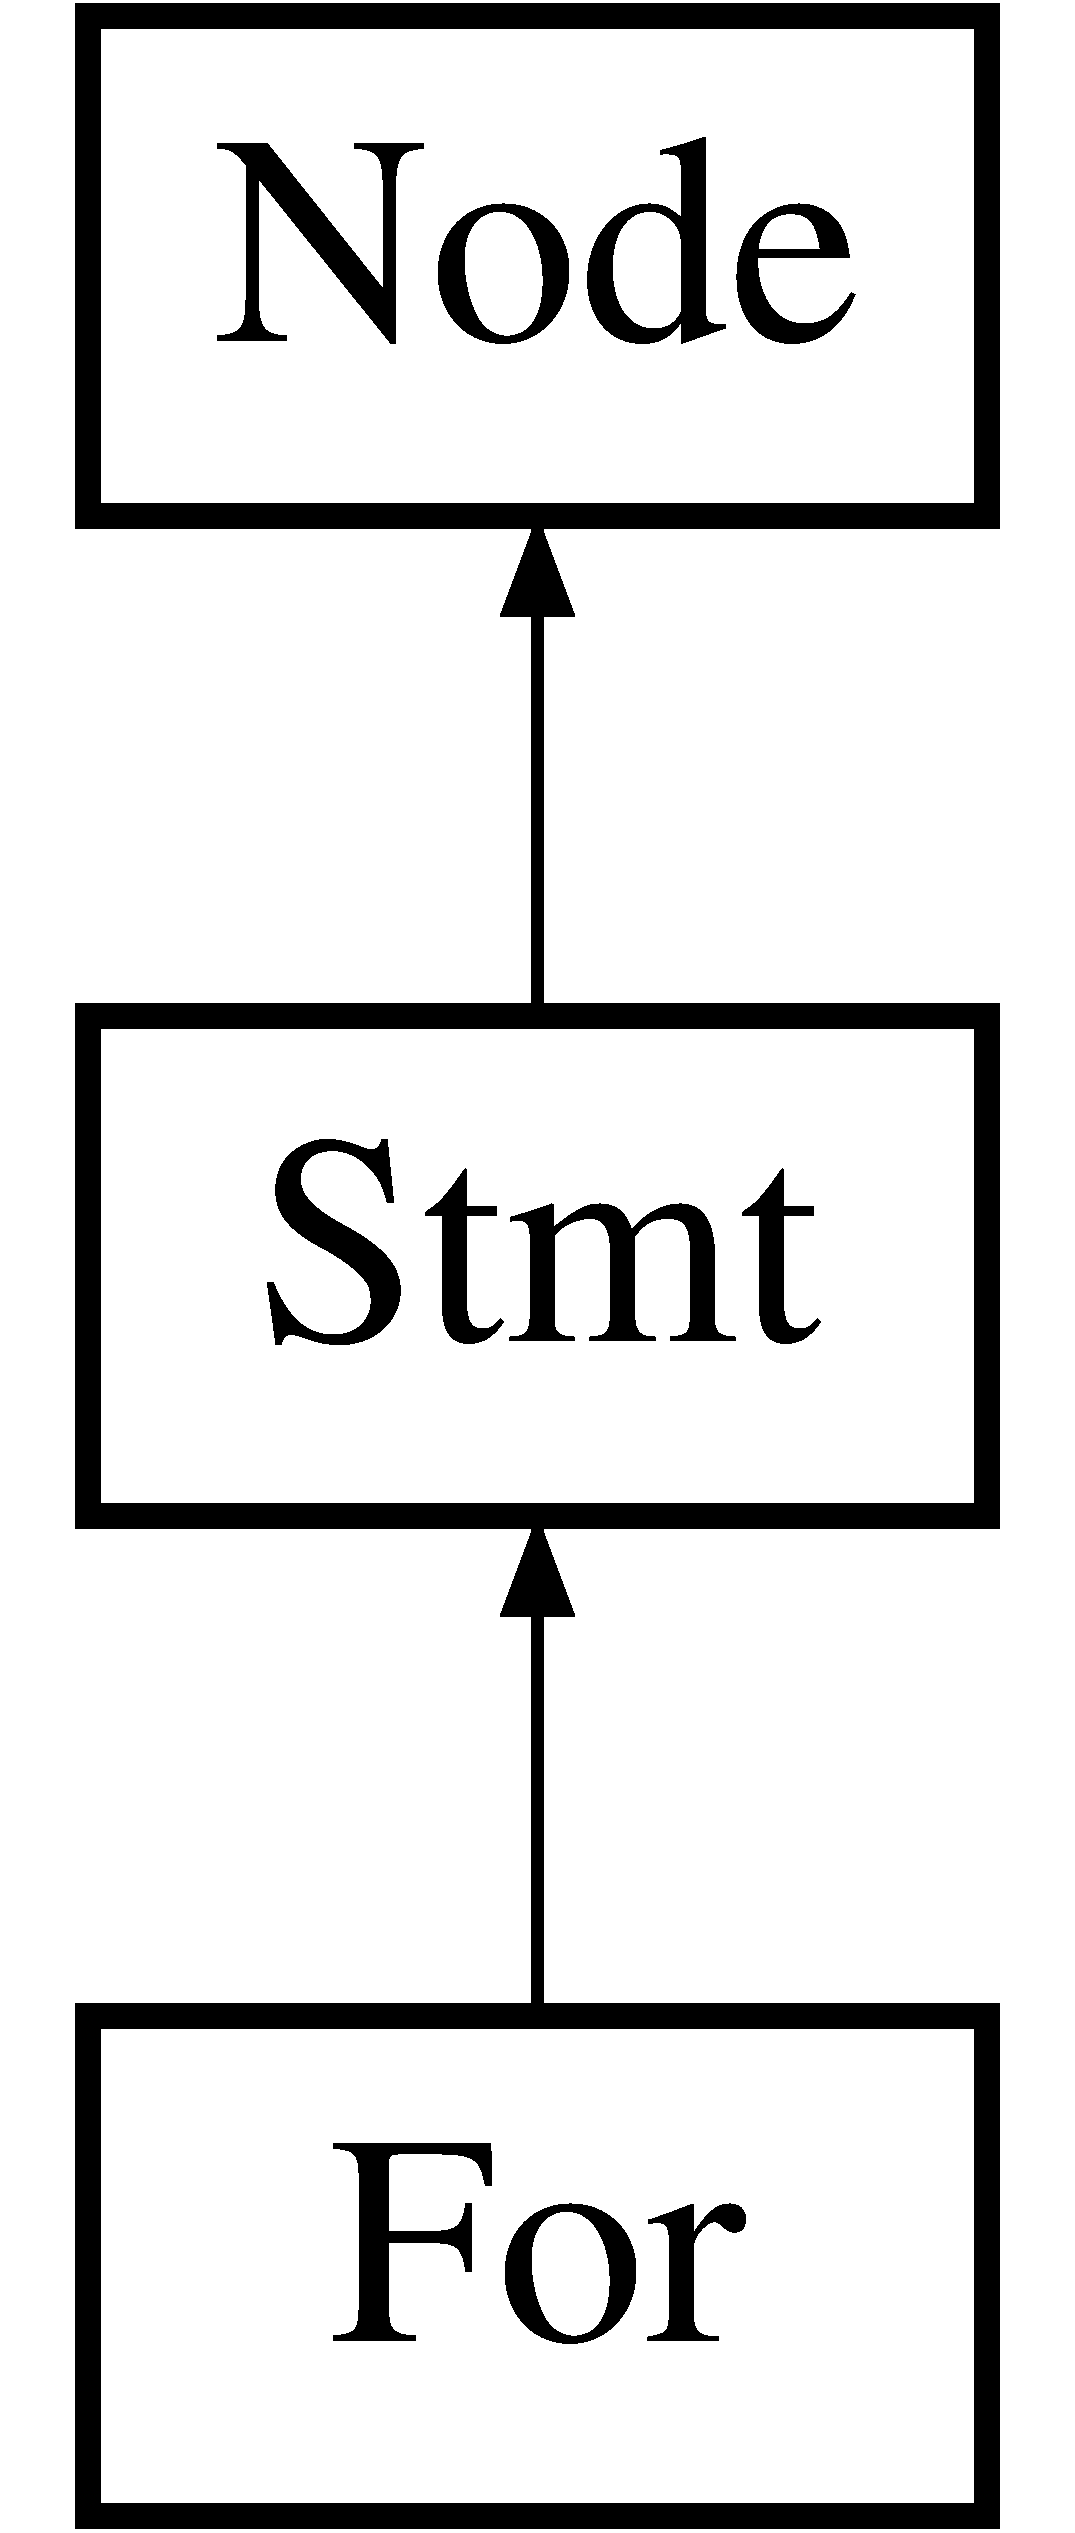
\includegraphics[height=3.000000cm]{class_for}
\end{center}
\end{figure}
\subsection*{Public 成员函数}
\begin{DoxyCompactItemize}
\item 
int \hyperlink{class_for_ad099d6d48c640dd5127285e59bbaba15}{execute} ()\hypertarget{class_for_ad099d6d48c640dd5127285e59bbaba15}{}\label{class_for_ad099d6d48c640dd5127285e59bbaba15}

\begin{DoxyCompactList}\small\item\em 执行for循环语句 \end{DoxyCompactList}\end{DoxyCompactItemize}
\subsection*{Public 属性}
\begin{DoxyCompactItemize}
\item 
\hyperlink{class_stmt}{Stmt} $\ast$ \hyperlink{class_for_a056889fe255686012e6a9197c2d514e7}{init\+Stmt}\hypertarget{class_for_a056889fe255686012e6a9197c2d514e7}{}\label{class_for_a056889fe255686012e6a9197c2d514e7}

\begin{DoxyCompactList}\small\item\em 初始化语句 \end{DoxyCompactList}\item 
\hyperlink{class_expr}{Expr} $\ast$ \hyperlink{class_for_a215e09b14cddca31190dc69cd783d886}{equal}\hypertarget{class_for_a215e09b14cddca31190dc69cd783d886}{}\label{class_for_a215e09b14cddca31190dc69cd783d886}

\begin{DoxyCompactList}\small\item\em 条件判断语句 \end{DoxyCompactList}\item 
\hyperlink{class_stmt}{Stmt} $\ast$ \hyperlink{class_for_a2d0ace8af086310ef5a11d9641dc81e6}{increasement}\hypertarget{class_for_a2d0ace8af086310ef5a11d9641dc81e6}{}\label{class_for_a2d0ace8af086310ef5a11d9641dc81e6}

\begin{DoxyCompactList}\small\item\em 循环条件增长语句 \end{DoxyCompactList}\item 
\hyperlink{class_stmt}{Stmt} $\ast$ \hyperlink{class_for_af269abab55eae120cccbd1c76b0c5011}{stmt}
\end{DoxyCompactItemize}
\subsection*{额外继承的成员函数}


\subsection{详细描述}
for循环语句类 

\subsection{类成员变量说明}
\index{For@{For}!stmt@{stmt}}
\index{stmt@{stmt}!For@{For}}
\subsubsection[{\texorpdfstring{stmt}{stmt}}]{\setlength{\rightskip}{0pt plus 5cm}{\bf Stmt}$\ast$ For\+::stmt}\hypertarget{class_for_af269abab55eae120cccbd1c76b0c5011}{}\label{class_for_af269abab55eae120cccbd1c76b0c5011}
循环体语句块 

该类的文档由以下文件生成\+:\begin{DoxyCompactItemize}
\item 
src/inter/stmt/For.\+h\item 
src/inter/stmt/For.\+cpp\end{DoxyCompactItemize}

\hypertarget{class_id}{}\section{Id Class Reference}
\label{class_id}\index{Id@{Id}}


变量的标示类  




{\ttfamily \#include $<$Id.\+h$>$}

Inheritance diagram for Id\+:\begin{figure}[H]
\begin{center}
\leavevmode
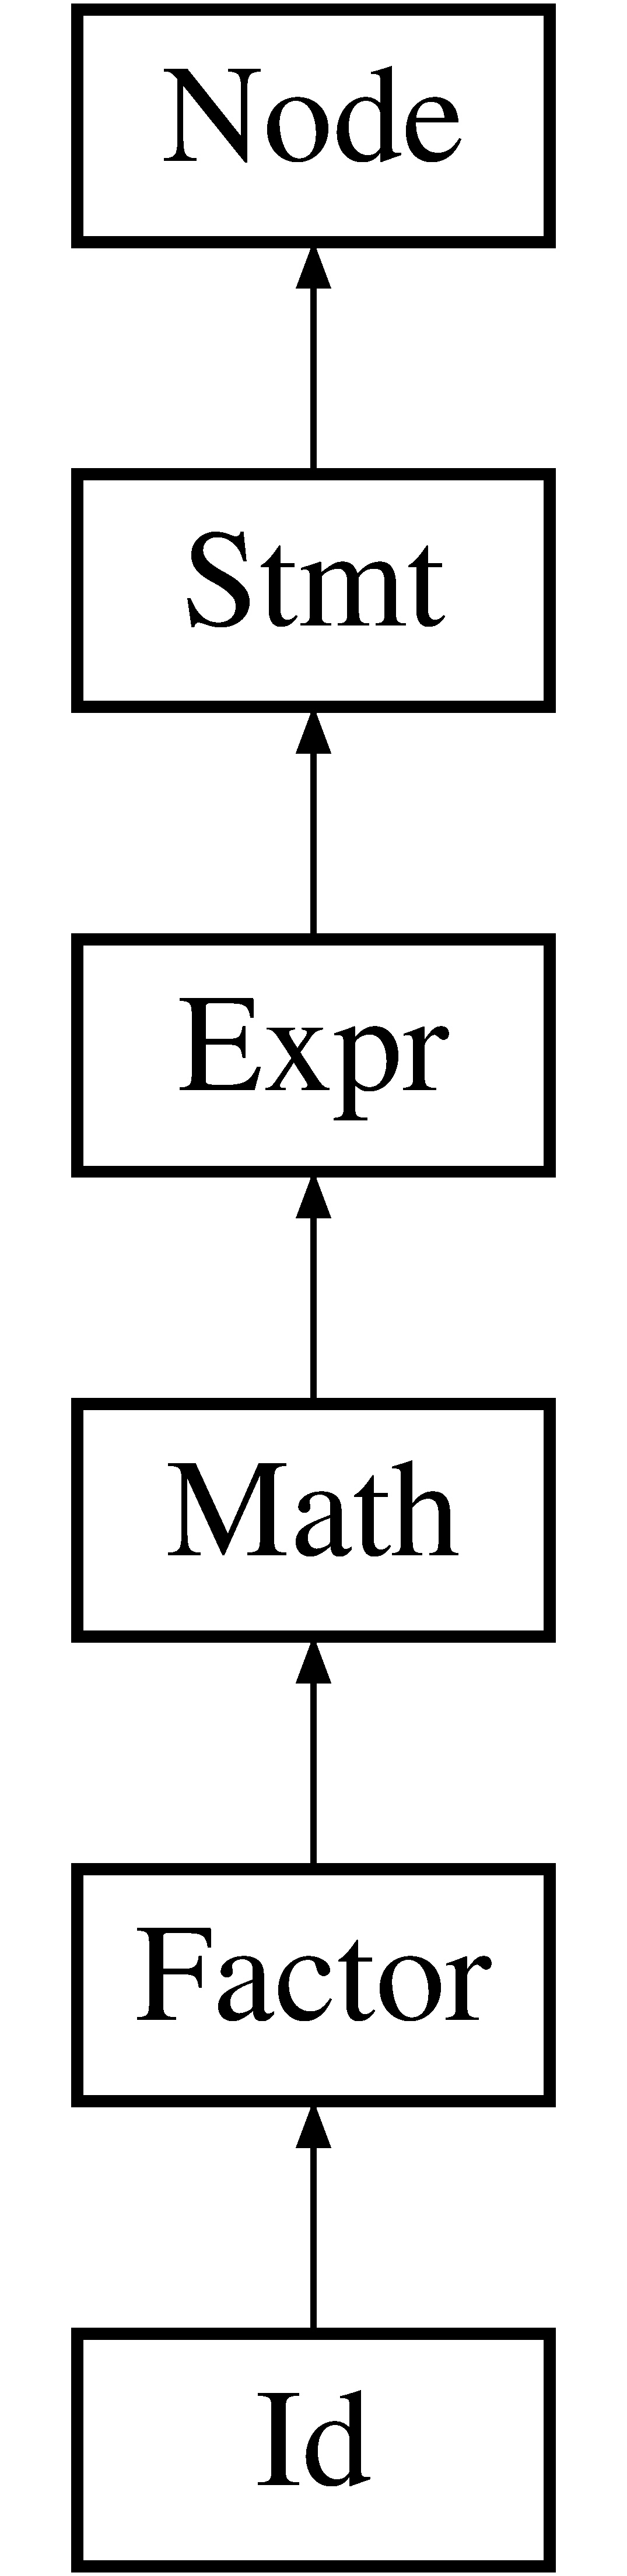
\includegraphics[height=6.000000cm]{class_id}
\end{center}
\end{figure}
\subsection*{Public Member Functions}
\begin{DoxyCompactItemize}
\item 
\hyperlink{class_id_a22122a40c4a61b6d2f7d20a3cc7c7275}{Id} (\hyperlink{class_word}{Word} $\ast$)
\item 
\mbox{\Hypertarget{class_id_ae43a9ffecbbc0ac4fd041b8e8e3c3de0}\label{class_id_ae43a9ffecbbc0ac4fd041b8e8e3c3de0}} 
int \hyperlink{class_id_ae43a9ffecbbc0ac4fd041b8e8e3c3de0}{execute} ()
\begin{DoxyCompactList}\small\item\em 执行返回id的值 \end{DoxyCompactList}\end{DoxyCompactItemize}
\subsection*{Public Attributes}
\begin{DoxyCompactItemize}
\item 
int \hyperlink{class_id_af7f7ed479b45ce150b88481b7b996e32}{value}
\end{DoxyCompactItemize}
\subsection*{Additional Inherited Members}


\subsection{Detailed Description}
变量的标示类 

\subsection{Constructor \& Destructor Documentation}
\mbox{\Hypertarget{class_id_a22122a40c4a61b6d2f7d20a3cc7c7275}\label{class_id_a22122a40c4a61b6d2f7d20a3cc7c7275}} 
\index{Id@{Id}!Id@{Id}}
\index{Id@{Id}!Id@{Id}}
\subsubsection{\texorpdfstring{Id()}{Id()}}
{\footnotesize\ttfamily Id\+::\+Id (\begin{DoxyParamCaption}\item[{\hyperlink{class_word}{Word} $\ast$}]{word }\end{DoxyParamCaption})}


\begin{DoxyParams}{Parameters}
{\em word} & \+: 变量的字 token \\
\hline
\end{DoxyParams}


\subsection{Member Data Documentation}
\mbox{\Hypertarget{class_id_af7f7ed479b45ce150b88481b7b996e32}\label{class_id_af7f7ed479b45ce150b88481b7b996e32}} 
\index{Id@{Id}!value@{value}}
\index{value@{value}!Id@{Id}}
\subsubsection{\texorpdfstring{value}{value}}
{\footnotesize\ttfamily int Id\+::value}

id 的值 

The documentation for this class was generated from the following files\+:\begin{DoxyCompactItemize}
\item 
src/inter/stmt/expr/Id.\+h\item 
src/inter/stmt/expr/Id.\+cpp\end{DoxyCompactItemize}

\hypertarget{class_if}{}\section{If类 参考}
\label{class_if}\index{If@{If}}


if语句类  




{\ttfamily \#include $<$If.\+h$>$}

类 If 继承关系图\+:\begin{figure}[H]
\begin{center}
\leavevmode
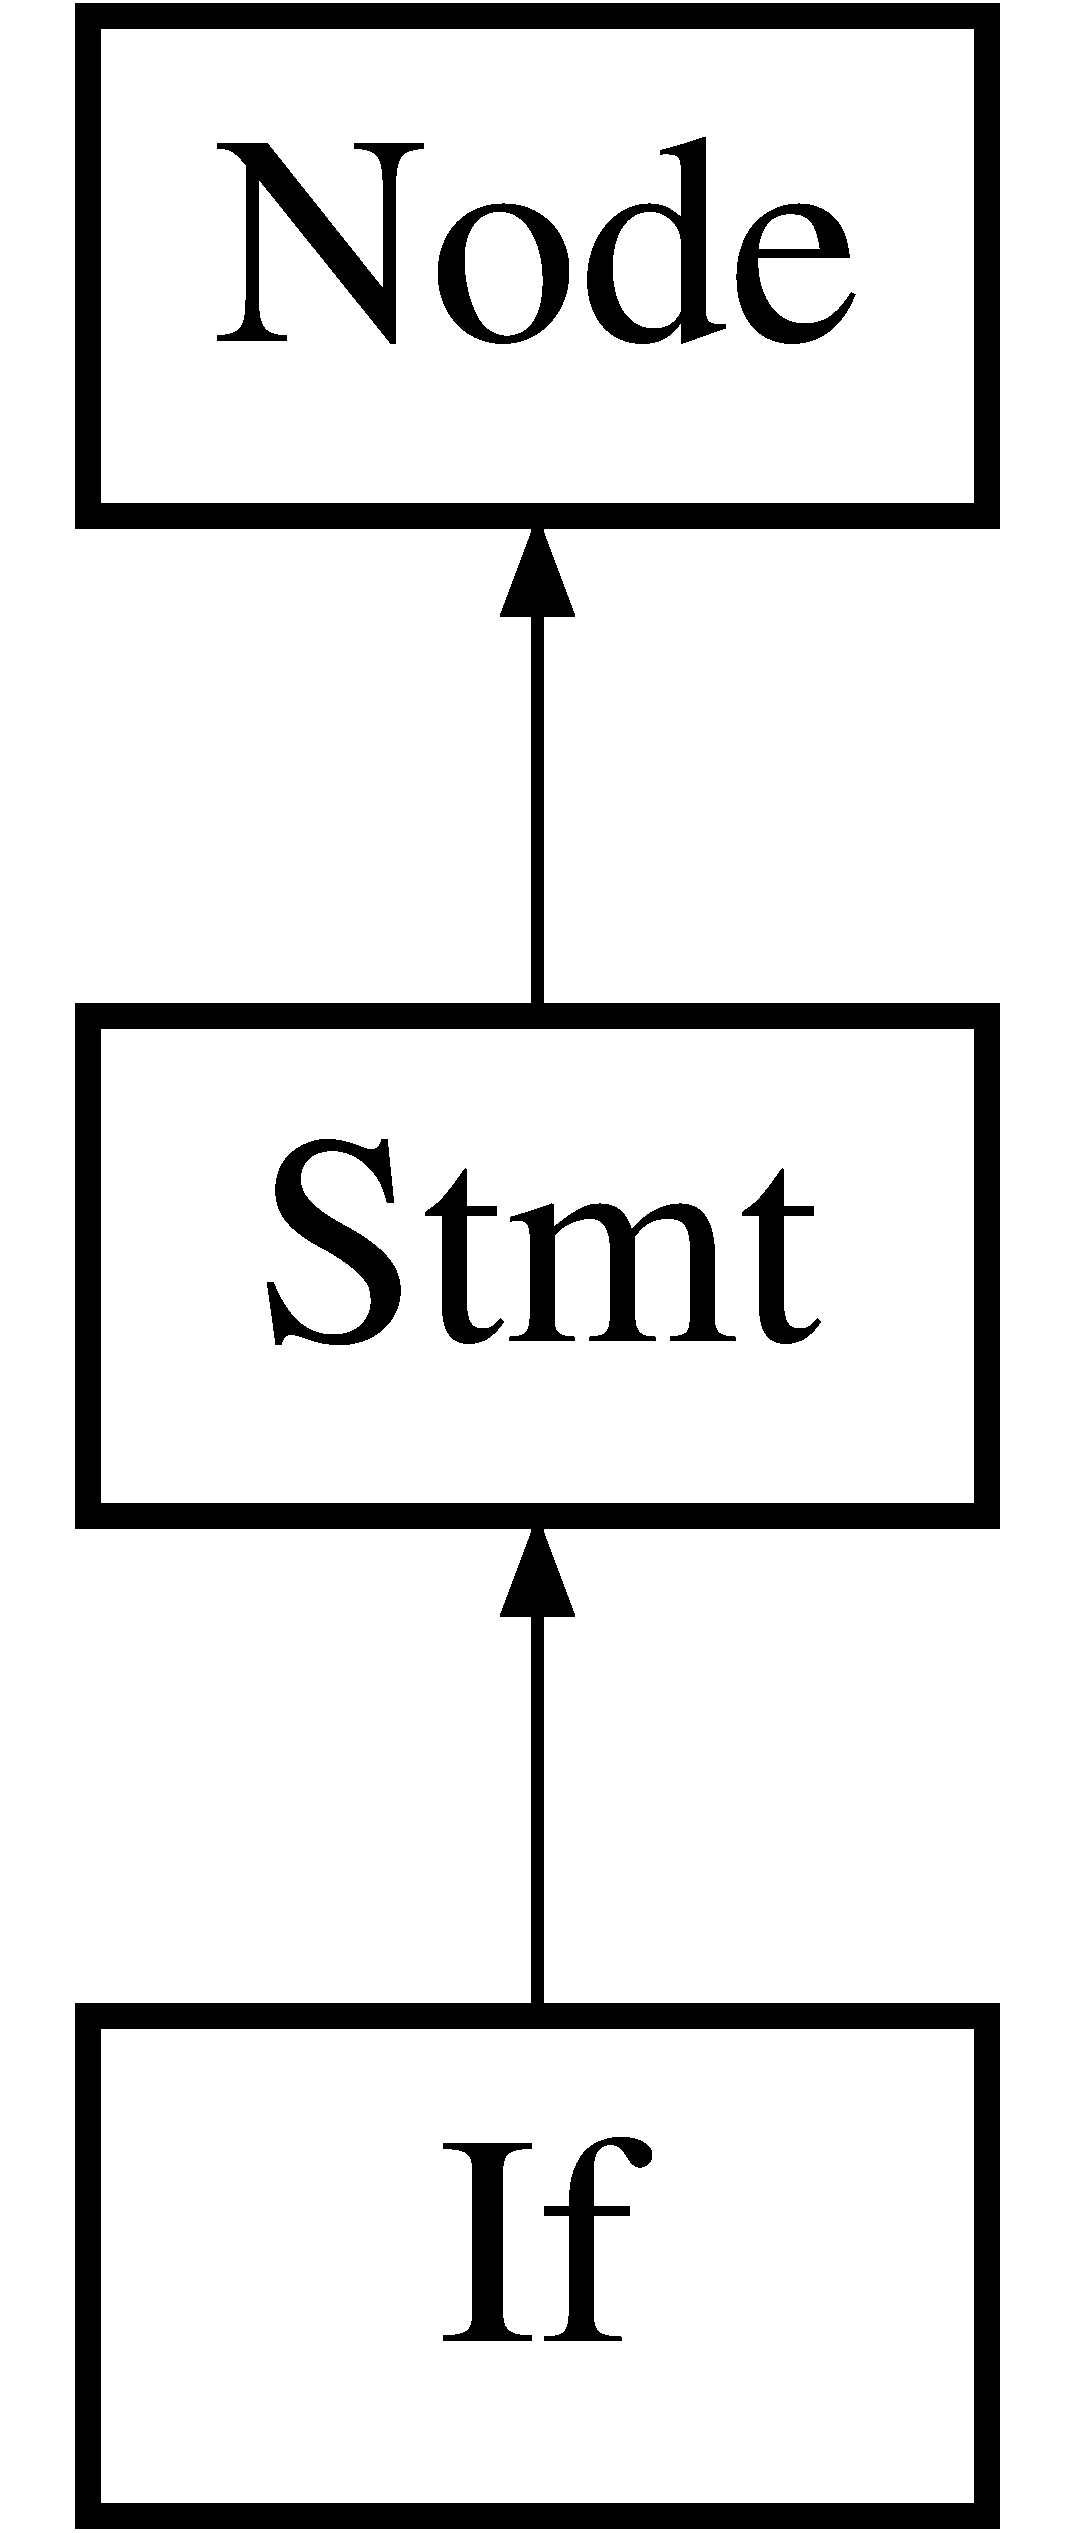
\includegraphics[height=3.000000cm]{class_if}
\end{center}
\end{figure}
\subsection*{Public 成员函数}
\begin{DoxyCompactItemize}
\item 
\mbox{\Hypertarget{class_if_aeadf929258ccd07a239879c118fb152f}\label{class_if_aeadf929258ccd07a239879c118fb152f}} 
int \hyperlink{class_if_aeadf929258ccd07a239879c118fb152f}{execute} ()
\begin{DoxyCompactList}\small\item\em 开始执行if语句 \end{DoxyCompactList}\item 
\hyperlink{class_if_a398387169436db838e9935b985a8f4a9}{If} (\hyperlink{class_expr}{Expr} $\ast$, \hyperlink{class_stmt}{Stmt} $\ast$, \hyperlink{class_stmt}{Stmt} $\ast$)
\end{DoxyCompactItemize}
\subsection*{Protected 属性}
\begin{DoxyCompactItemize}
\item 
\mbox{\Hypertarget{class_if_a84f2d73109cd8030fcc244ef741b5803}\label{class_if_a84f2d73109cd8030fcc244ef741b5803}} 
\hyperlink{class_expr}{Expr} $\ast$ \hyperlink{class_if_a84f2d73109cd8030fcc244ef741b5803}{equality}
\begin{DoxyCompactList}\small\item\em if判断表达式 \end{DoxyCompactList}\item 
\mbox{\Hypertarget{class_if_a3ece7870e5d5b11dd42457e22af00a72}\label{class_if_a3ece7870e5d5b11dd42457e22af00a72}} 
\hyperlink{class_stmt}{Stmt} $\ast$ \hyperlink{class_if_a3ece7870e5d5b11dd42457e22af00a72}{stmt1}
\begin{DoxyCompactList}\small\item\em if语句块部分 \end{DoxyCompactList}\item 
\mbox{\Hypertarget{class_if_aaf8a095b5a986832928ebdcdb263d41c}\label{class_if_aaf8a095b5a986832928ebdcdb263d41c}} 
\hyperlink{class_stmt}{Stmt} $\ast$ \hyperlink{class_if_aaf8a095b5a986832928ebdcdb263d41c}{stmt2}
\begin{DoxyCompactList}\small\item\em else语句块部分,没有则为\+N\+U\+LL \end{DoxyCompactList}\end{DoxyCompactItemize}
\subsection*{额外继承的成员函数}


\subsection{详细描述}
if语句类 

\subsection{构造及析构函数说明}
\mbox{\Hypertarget{class_if_a398387169436db838e9935b985a8f4a9}\label{class_if_a398387169436db838e9935b985a8f4a9}} 
\index{If@{If}!If@{If}}
\index{If@{If}!If@{If}}
\subsubsection{\texorpdfstring{If()}{If()}}
{\footnotesize\ttfamily If\+::\+If (\begin{DoxyParamCaption}\item[{\hyperlink{class_expr}{Expr} $\ast$}]{equality1,  }\item[{\hyperlink{class_stmt}{Stmt} $\ast$}]{stmt3,  }\item[{\hyperlink{class_stmt}{Stmt} $\ast$}]{stmt4 }\end{DoxyParamCaption})}


\begin{DoxyParams}{参数}
{\em expr} & \+: 条件表达式 \\
\hline
{\em stmt1} & \+: if 语句块 \\
\hline
{\em stmt2} & \+: else 语句块 \\
\hline
\end{DoxyParams}


该类的文档由以下文件生成\+:\begin{DoxyCompactItemize}
\item 
src/inter/stmt/If.\+h\item 
src/inter/stmt/If.\+cpp\end{DoxyCompactItemize}

\hypertarget{class_lexer}{}\section{Lexer类 参考}
\label{class_lexer}\index{Lexer@{Lexer}}


词法分析器  




{\ttfamily \#include $<$Lexer.\+h$>$}

\subsection*{Public 成员函数}
\begin{DoxyCompactItemize}
\item 
void \hyperlink{class_lexer_ae96c693bf6eba38f21adab5fc94c18b1}{reserve} (\hyperlink{class_word}{Word} $\ast$)\hypertarget{class_lexer_ae96c693bf6eba38f21adab5fc94c18b1}{}\label{class_lexer_ae96c693bf6eba38f21adab5fc94c18b1}

\begin{DoxyCompactList}\small\item\em 录入保留字 \end{DoxyCompactList}\item 
bool \hyperlink{class_lexer_a3fafe4fb32f4da95a08d1062996b0409}{set\+File} ()\hypertarget{class_lexer_a3fafe4fb32f4da95a08d1062996b0409}{}\label{class_lexer_a3fafe4fb32f4da95a08d1062996b0409}

\begin{DoxyCompactList}\small\item\em 设置源文件 \end{DoxyCompactList}\item 
void \hyperlink{class_lexer_a5c91a26ad6b4294bf7bb8d4c46ea529b}{readch} ()\hypertarget{class_lexer_a5c91a26ad6b4294bf7bb8d4c46ea529b}{}\label{class_lexer_a5c91a26ad6b4294bf7bb8d4c46ea529b}

\begin{DoxyCompactList}\small\item\em 获取下一个字符 \end{DoxyCompactList}\item 
bool \hyperlink{class_lexer_acbe68a5d98ebc3b3a87fd27f000030a5}{readch} (char c)
\begin{DoxyCompactList}\small\item\em look ahead 方法 \end{DoxyCompactList}\item 
void \hyperlink{class_lexer_ae28380e5c67144a1aeaf37f33ab11fb2}{back} ()\hypertarget{class_lexer_ae28380e5c67144a1aeaf37f33ab11fb2}{}\label{class_lexer_ae28380e5c67144a1aeaf37f33ab11fb2}

\begin{DoxyCompactList}\small\item\em 字符回退 \end{DoxyCompactList}\item 
\hyperlink{class_token}{Token} $\ast$ \hyperlink{class_lexer_a2085b8262f6237de60583375ee2731f4}{scan} ()
\begin{DoxyCompactList}\small\item\em 扫描下一个 token \end{DoxyCompactList}\item 
\hyperlink{class_lexer_a2752a2b16cc1ffbcb8fc3e82e95bf331}{Lexer} ()\hypertarget{class_lexer_a2752a2b16cc1ffbcb8fc3e82e95bf331}{}\label{class_lexer_a2752a2b16cc1ffbcb8fc3e82e95bf331}

\begin{DoxyCompactList}\small\item\em 构造\+Lexer 初始化保留字 \end{DoxyCompactList}\end{DoxyCompactItemize}
\subsection*{静态 Public 成员函数}
\begin{DoxyCompactItemize}
\item 
static void {\bfseries line\+Incre} ()\hypertarget{class_lexer_a48478c1d6556ce949e7808bf3e2604b7}{}\label{class_lexer_a48478c1d6556ce949e7808bf3e2604b7}

\item 
static int \hyperlink{class_lexer_a0ede40225695d9eb9b42d275584cf8f0}{get\+Line} ()\hypertarget{class_lexer_a0ede40225695d9eb9b42d275584cf8f0}{}\label{class_lexer_a0ede40225695d9eb9b42d275584cf8f0}

\begin{DoxyCompactList}\small\item\em 获取 token 行号 \end{DoxyCompactList}\end{DoxyCompactItemize}
\subsection*{Private 成员函数}
\begin{DoxyCompactItemize}
\item 
void \hyperlink{class_lexer_abb0f5b7f1e6fd685c8c8e9074553c67f}{read} (char $\ast$)
\item 
\hyperlink{class_token}{Token} $\ast$ \hyperlink{class_lexer_aa5f52af80cfc8de7841d2ac6bc736662}{first\+Scan} ()\hypertarget{class_lexer_aa5f52af80cfc8de7841d2ac6bc736662}{}\label{class_lexer_aa5f52af80cfc8de7841d2ac6bc736662}

\begin{DoxyCompactList}\small\item\em 构建根块 \end{DoxyCompactList}\item 
\hyperlink{class_token}{Token} $\ast$ \hyperlink{class_lexer_a28eb3e3a349bcbc7a0b03e16bb42192f}{last\+Scan} ()\hypertarget{class_lexer_a28eb3e3a349bcbc7a0b03e16bb42192f}{}\label{class_lexer_a28eb3e3a349bcbc7a0b03e16bb42192f}

\begin{DoxyCompactList}\small\item\em 构建根块 \end{DoxyCompactList}\end{DoxyCompactItemize}
\subsection*{Private 属性}
\begin{DoxyCompactItemize}
\item 
std\+::ifstream \hyperlink{class_lexer_a606dd5cec5ec316ca1b1df40823fb853}{input\+\_\+file}\hypertarget{class_lexer_a606dd5cec5ec316ca1b1df40823fb853}{}\label{class_lexer_a606dd5cec5ec316ca1b1df40823fb853}

\begin{DoxyCompactList}\small\item\em 输入文件 \end{DoxyCompactList}\item 
char \hyperlink{class_lexer_a372c56c466c70d808bdcdb11e94bd914}{buffer} \mbox{[}4097\mbox{]}\hypertarget{class_lexer_a372c56c466c70d808bdcdb11e94bd914}{}\label{class_lexer_a372c56c466c70d808bdcdb11e94bd914}

\begin{DoxyCompactList}\small\item\em 缓冲区 \end{DoxyCompactList}\item 
int \hyperlink{class_lexer_a266317e9b89ad0e681fdb21032ef00f8}{index} = 0\hypertarget{class_lexer_a266317e9b89ad0e681fdb21032ef00f8}{}\label{class_lexer_a266317e9b89ad0e681fdb21032ef00f8}

\begin{DoxyCompactList}\small\item\em 缓冲区读取指针 \end{DoxyCompactList}\item 
char \hyperlink{class_lexer_a1c13ae056a34e7ec483c561152bb8d49}{peek} = \textquotesingle{} \textquotesingle{}\hypertarget{class_lexer_a1c13ae056a34e7ec483c561152bb8d49}{}\label{class_lexer_a1c13ae056a34e7ec483c561152bb8d49}

\begin{DoxyCompactList}\small\item\em 当前扫描到的字符 \end{DoxyCompactList}\item 
std\+::map$<$ std\+::string, \hyperlink{class_word}{Word} $>$ \hyperlink{class_lexer_add52df03b8546bfe059f4e1832141c16}{words}\hypertarget{class_lexer_add52df03b8546bfe059f4e1832141c16}{}\label{class_lexer_add52df03b8546bfe059f4e1832141c16}

\begin{DoxyCompactList}\small\item\em 单词保留区 \end{DoxyCompactList}\item 
bool \hyperlink{class_lexer_a123d0134daef2ce492f0707342456afc}{read\+Finished} = false\hypertarget{class_lexer_a123d0134daef2ce492f0707342456afc}{}\label{class_lexer_a123d0134daef2ce492f0707342456afc}

\begin{DoxyCompactList}\small\item\em 标记是否到达文件末尾 \end{DoxyCompactList}\end{DoxyCompactItemize}
\subsection*{静态 Private 属性}
\begin{DoxyCompactItemize}
\item 
static const int \hyperlink{class_lexer_af8222e02dc3180feb942b4a6d3083a22}{B\+U\+F\+F\+E\+R\+\_\+\+L\+E\+N\+T\+H\+GH} = 4096\hypertarget{class_lexer_af8222e02dc3180feb942b4a6d3083a22}{}\label{class_lexer_af8222e02dc3180feb942b4a6d3083a22}

\begin{DoxyCompactList}\small\item\em 读取文件的缓冲区大小 \end{DoxyCompactList}\item 
static int \hyperlink{class_lexer_a35d0802ee5cced4c5294fb6dc77ad2f4}{line} = 1\hypertarget{class_lexer_a35d0802ee5cced4c5294fb6dc77ad2f4}{}\label{class_lexer_a35d0802ee5cced4c5294fb6dc77ad2f4}

\begin{DoxyCompactList}\small\item\em 当前行 \end{DoxyCompactList}\end{DoxyCompactItemize}


\subsection{详细描述}
词法分析器 

该类用于把源文件分析成token流, 便于语法分析时对元素的提取 

\subsection{成员函数说明}
\index{Lexer@{Lexer}!read@{read}}
\index{read@{read}!Lexer@{Lexer}}
\subsubsection[{\texorpdfstring{read(char $\ast$)}{read(char *)}}]{\setlength{\rightskip}{0pt plus 5cm}void Lexer\+::read (
\begin{DoxyParamCaption}
\item[{char $\ast$}]{ch}
\end{DoxyParamCaption}
)\hspace{0.3cm}{\ttfamily [private]}}\hypertarget{class_lexer_abb0f5b7f1e6fd685c8c8e9074553c67f}{}\label{class_lexer_abb0f5b7f1e6fd685c8c8e9074553c67f}
读取文件进入buffer中 \index{Lexer@{Lexer}!readch@{readch}}
\index{readch@{readch}!Lexer@{Lexer}}
\subsubsection[{\texorpdfstring{readch(char c)}{readch(char c)}}]{\setlength{\rightskip}{0pt plus 5cm}bool Lexer\+::readch (
\begin{DoxyParamCaption}
\item[{char}]{c}
\end{DoxyParamCaption}
)}\hypertarget{class_lexer_acbe68a5d98ebc3b3a87fd27f000030a5}{}\label{class_lexer_acbe68a5d98ebc3b3a87fd27f000030a5}


look ahead 方法 


\begin{DoxyParams}{参数}
{\em c} & 判断下一个字符是否为c \\
\hline
\end{DoxyParams}
\index{Lexer@{Lexer}!scan@{scan}}
\index{scan@{scan}!Lexer@{Lexer}}
\subsubsection[{\texorpdfstring{scan()}{scan()}}]{\setlength{\rightskip}{0pt plus 5cm}{\bf Token} $\ast$ Lexer\+::scan (
\begin{DoxyParamCaption}
{}
\end{DoxyParamCaption}
)}\hypertarget{class_lexer_a2085b8262f6237de60583375ee2731f4}{}\label{class_lexer_a2085b8262f6237de60583375ee2731f4}


扫描下一个 token 

从缓冲区中~\newline
首先跳过空白和注释~\newline
然后检查是否发现特殊符号~\newline
接着检查保留字的出现情况~\newline
返回相应的 token~\newline


该类的文档由以下文件生成\+:\begin{DoxyCompactItemize}
\item 
src/lexer/Lexer.\+h\item 
src/lexer/Lexer.\+cpp\end{DoxyCompactItemize}

\hypertarget{class_math}{}\section{Math Class Reference}
\label{class_math}\index{Math@{Math}}


数学运算的根类  




{\ttfamily \#include $<$Math.\+h$>$}

Inheritance diagram for Math\+:\begin{figure}[H]
\begin{center}
\leavevmode
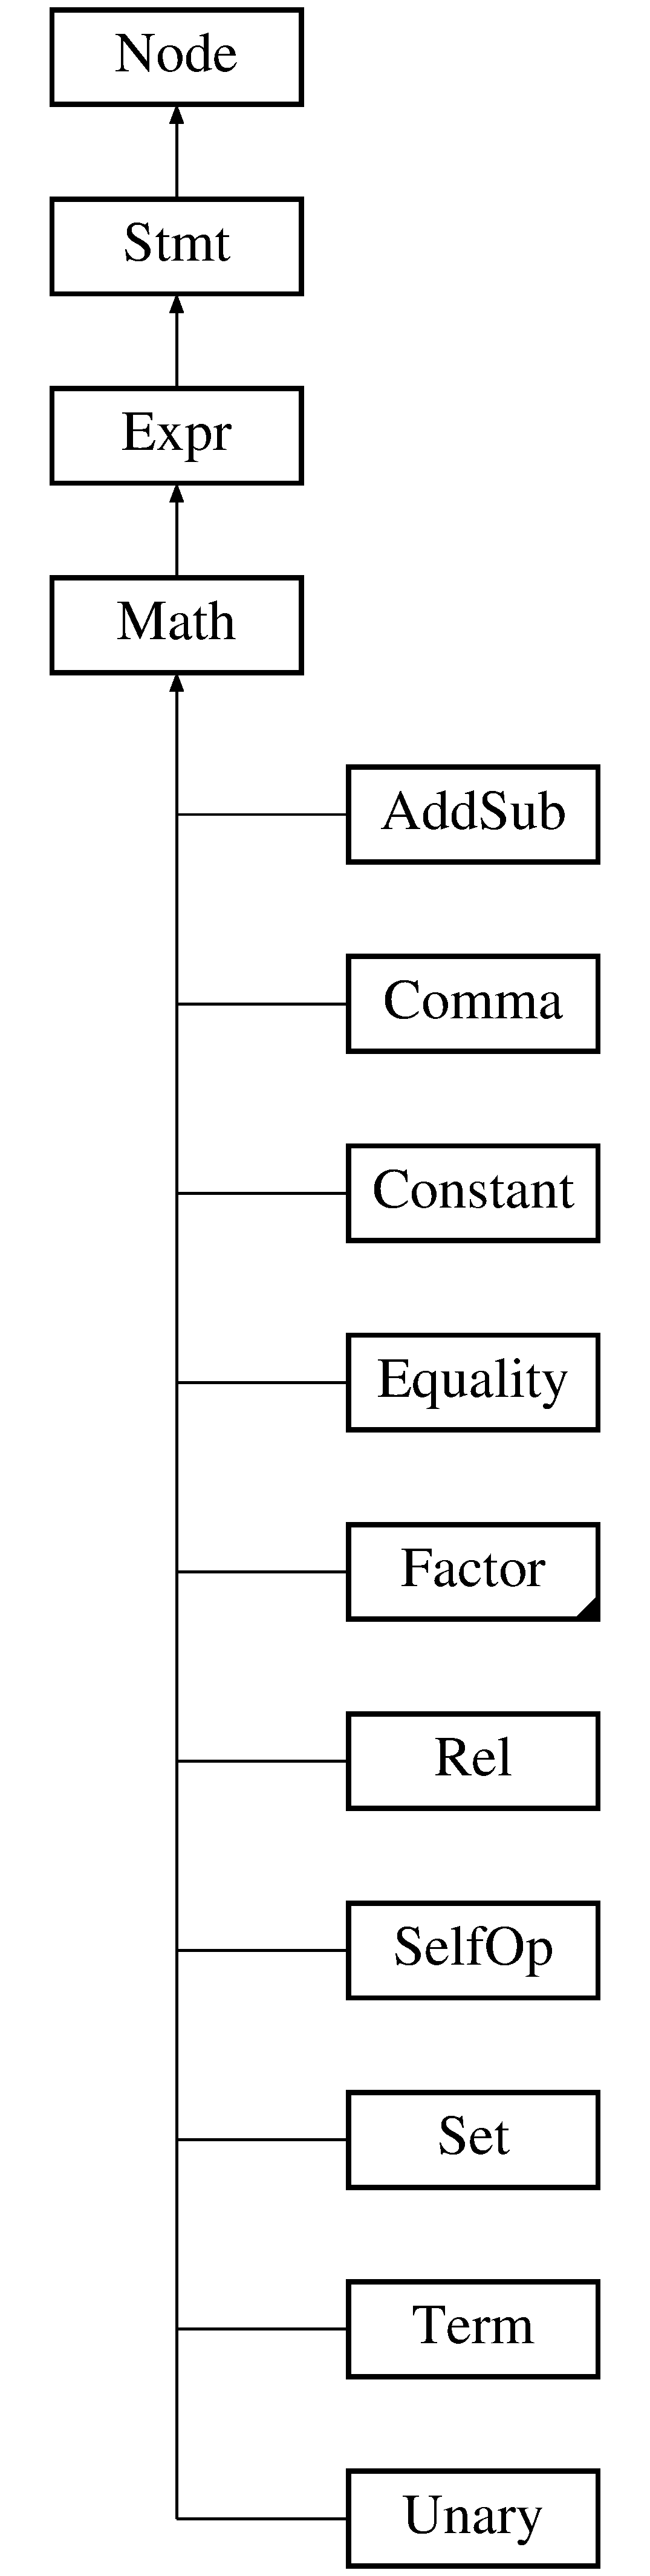
\includegraphics[height=12.000000cm]{class_math}
\end{center}
\end{figure}
\subsection*{Public Member Functions}
\begin{DoxyCompactItemize}
\item 
\hyperlink{class_math_af045a09f80d73b385d902041bc5cf41e}{Math} (\hyperlink{class_token}{Token} $\ast$token, \hyperlink{class_expr}{Expr} $\ast$expr1, \hyperlink{class_expr}{Expr} $\ast$expr2)
\end{DoxyCompactItemize}
\subsection*{Public Attributes}
\begin{DoxyCompactItemize}
\item 
\hyperlink{class_expr}{Expr} $\ast$ \hyperlink{class_math_a551d177c9245212a8b5374ea1e4024ea}{expr\+\_\+l}
\begin{DoxyCompactList}\small\item\em 左表达式 \end{DoxyCompactList}\item 
\hyperlink{class_expr}{Expr} $\ast$ \hyperlink{class_math_a2e2eb1f4f47fd10466db783b20183307}{expr\+\_\+r}
\end{DoxyCompactItemize}
\subsection*{Additional Inherited Members}


\subsection{Detailed Description}
数学运算的根类 

\subsection{Constructor \& Destructor Documentation}
\mbox{\Hypertarget{class_math_af045a09f80d73b385d902041bc5cf41e}\label{class_math_af045a09f80d73b385d902041bc5cf41e}} 
\index{Math@{Math}!Math@{Math}}
\index{Math@{Math}!Math@{Math}}
\subsubsection{\texorpdfstring{Math()}{Math()}}
{\footnotesize\ttfamily Math\+::\+Math (\begin{DoxyParamCaption}\item[{\hyperlink{class_token}{Token} $\ast$}]{token,  }\item[{\hyperlink{class_expr}{Expr} $\ast$}]{expr1,  }\item[{\hyperlink{class_expr}{Expr} $\ast$}]{expr2 }\end{DoxyParamCaption})}


\begin{DoxyParams}{Parameters}
{\em token} & \+: 运算符 \\
\hline
{\em expr1} & \+: 左表达式 \\
\hline
{\em expr2} & \+: 右表达式 \\
\hline
\end{DoxyParams}


\subsection{Member Data Documentation}
\mbox{\Hypertarget{class_math_a551d177c9245212a8b5374ea1e4024ea}\label{class_math_a551d177c9245212a8b5374ea1e4024ea}} 
\index{Math@{Math}!expr\+\_\+l@{expr\+\_\+l}}
\index{expr\+\_\+l@{expr\+\_\+l}!Math@{Math}}
\subsubsection{\texorpdfstring{expr\+\_\+l}{expr\_l}}
{\footnotesize\ttfamily \hyperlink{class_expr}{Expr}$\ast$ Math\+::expr\+\_\+l}



左表达式 

\mbox{\Hypertarget{class_math_a2e2eb1f4f47fd10466db783b20183307}\label{class_math_a2e2eb1f4f47fd10466db783b20183307}} 
\index{Math@{Math}!expr\+\_\+r@{expr\+\_\+r}}
\index{expr\+\_\+r@{expr\+\_\+r}!Math@{Math}}
\subsubsection{\texorpdfstring{expr\+\_\+r}{expr\_r}}
{\footnotesize\ttfamily \hyperlink{class_expr}{Expr}$\ast$ Math\+::expr\+\_\+r}

右表达式 

The documentation for this class was generated from the following files\+:\begin{DoxyCompactItemize}
\item 
src/inter/stmt/expr/\hyperlink{_math_8h}{Math.\+h}\item 
src/inter/stmt/expr/\hyperlink{_math_8cpp}{Math.\+cpp}\end{DoxyCompactItemize}

\hypertarget{class_node}{}\section{Node类 参考}
\label{class_node}\index{Node@{Node}}


Node类  




{\ttfamily \#include $<$Node.\+h$>$}

类 Node 继承关系图\+:\begin{figure}[H]
\begin{center}
\leavevmode
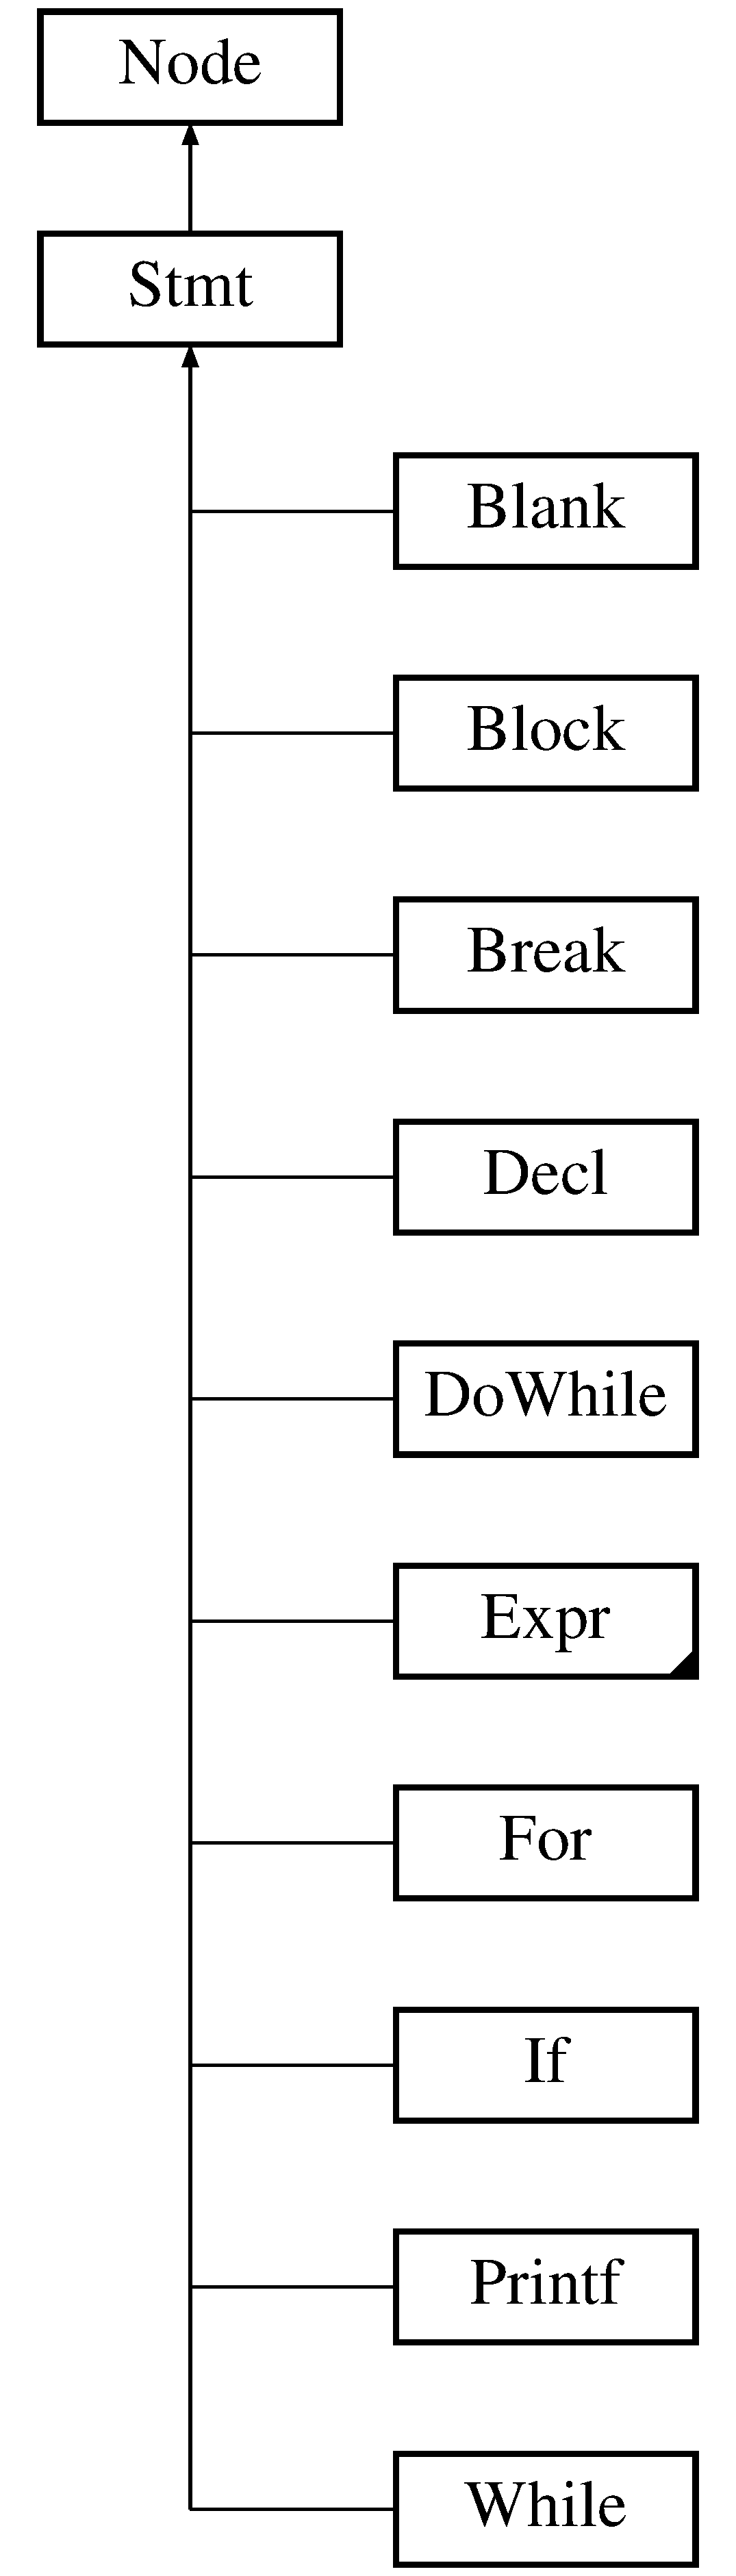
\includegraphics[height=12.000000cm]{class_node}
\end{center}
\end{figure}
\subsection*{Public 成员函数}
\begin{DoxyCompactItemize}
\item 
\mbox{\Hypertarget{class_node_ad7a34779cad45d997bfd6d3d8043c75f}\label{class_node_ad7a34779cad45d997bfd6d3d8043c75f}} 
\hyperlink{class_node_ad7a34779cad45d997bfd6d3d8043c75f}{Node} ()
\begin{DoxyCompactList}\small\item\em 用于初始化节点行号 \end{DoxyCompactList}\end{DoxyCompactItemize}
\subsection*{Public 属性}
\begin{DoxyCompactItemize}
\item 
int \hyperlink{class_node_a8e50263ff9416be77e26edfbf6b926a1}{lexline} = 0
\end{DoxyCompactItemize}
\subsection*{Protected 成员函数}
\begin{DoxyCompactItemize}
\item 
\mbox{\Hypertarget{class_node_aa1bb6c155277eb2c073a60c00674b8b6}\label{class_node_aa1bb6c155277eb2c073a60c00674b8b6}} 
void \hyperlink{class_node_aa1bb6c155277eb2c073a60c00674b8b6}{error} (std\+::string)
\begin{DoxyCompactList}\small\item\em $<$ 节点抛出异常 \end{DoxyCompactList}\end{DoxyCompactItemize}


\subsection{详细描述}
Node类 

所有的语句内容都算是抽象语法树中的一个节点 所有的语句与表达式都是该类的子类 

\subsection{类成员变量说明}
\mbox{\Hypertarget{class_node_a8e50263ff9416be77e26edfbf6b926a1}\label{class_node_a8e50263ff9416be77e26edfbf6b926a1}} 
\index{Node@{Node}!lexline@{lexline}}
\index{lexline@{lexline}!Node@{Node}}
\subsubsection{\texorpdfstring{lexline}{lexline}}
{\footnotesize\ttfamily int Node\+::lexline = 0}

该节点位于的行号 

该类的文档由以下文件生成\+:\begin{DoxyCompactItemize}
\item 
src/inter/Node.\+h\item 
src/inter/Node.\+cpp\end{DoxyCompactItemize}

\hypertarget{class_num}{}\section{Num Class Reference}
\label{class_num}\index{Num@{Num}}


{\ttfamily \#include $<$Num.\+h$>$}

Inheritance diagram for Num\+:\begin{figure}[H]
\begin{center}
\leavevmode
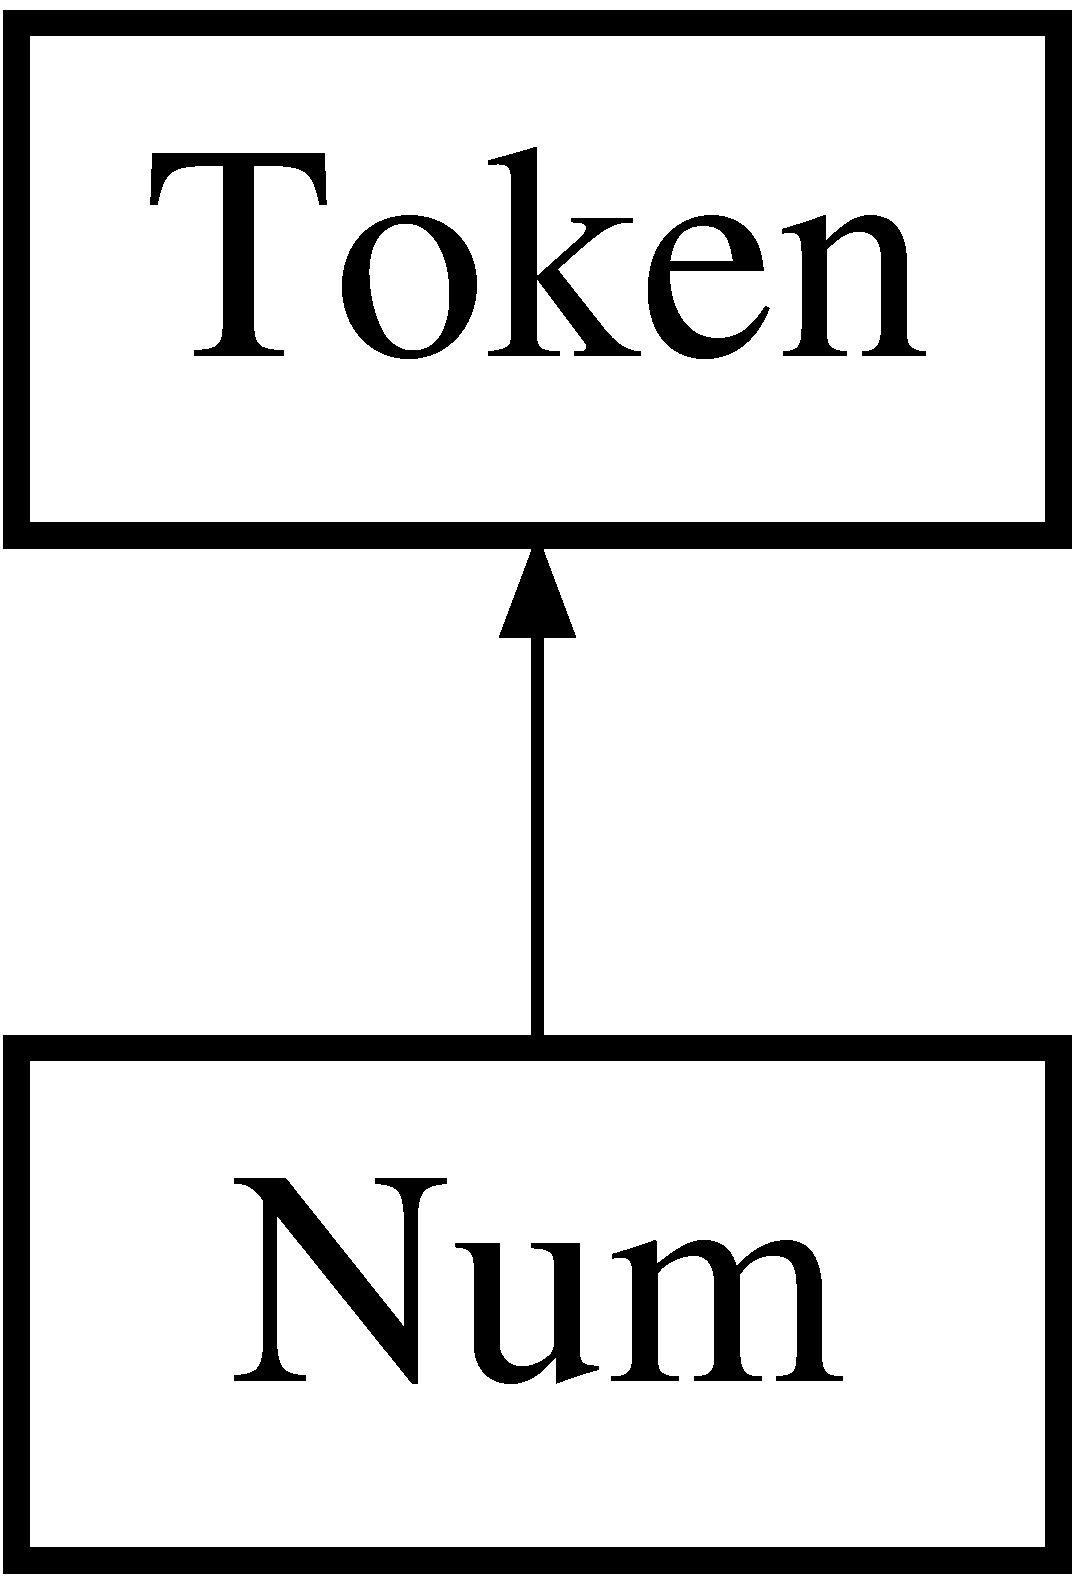
\includegraphics[height=2.000000cm]{class_num}
\end{center}
\end{figure}
\subsection*{Public Member Functions}
\begin{DoxyCompactItemize}
\item 
\hyperlink{class_num_afc0c5a6bc449547b300aa036e70eda2d}{Num} (int v)
\item 
std\+::string \hyperlink{class_num_aec8ab507b42f2080a8cc197f45f0c935}{to\+String} ()
\end{DoxyCompactItemize}
\subsection*{Public Attributes}
\begin{DoxyCompactItemize}
\item 
int \hyperlink{class_num_a40cb04ca1ed295495a2e4b358b984fb8}{value}
\end{DoxyCompactItemize}


\subsection{Constructor \& Destructor Documentation}
\mbox{\Hypertarget{class_num_afc0c5a6bc449547b300aa036e70eda2d}\label{class_num_afc0c5a6bc449547b300aa036e70eda2d}} 
\index{Num@{Num}!Num@{Num}}
\index{Num@{Num}!Num@{Num}}
\subsubsection{\texorpdfstring{Num()}{Num()}}
{\footnotesize\ttfamily Num\+::\+Num (\begin{DoxyParamCaption}\item[{int}]{v }\end{DoxyParamCaption})}



\subsection{Member Function Documentation}
\mbox{\Hypertarget{class_num_aec8ab507b42f2080a8cc197f45f0c935}\label{class_num_aec8ab507b42f2080a8cc197f45f0c935}} 
\index{Num@{Num}!to\+String@{to\+String}}
\index{to\+String@{to\+String}!Num@{Num}}
\subsubsection{\texorpdfstring{to\+String()}{toString()}}
{\footnotesize\ttfamily std\+::string Num\+::to\+String (\begin{DoxyParamCaption}{ }\end{DoxyParamCaption})\hspace{0.3cm}{\ttfamily [virtual]}}



Reimplemented from \hyperlink{class_token_a8863381edabce7bc1e92473b445ba81f}{Token}.



\subsection{Member Data Documentation}
\mbox{\Hypertarget{class_num_a40cb04ca1ed295495a2e4b358b984fb8}\label{class_num_a40cb04ca1ed295495a2e4b358b984fb8}} 
\index{Num@{Num}!value@{value}}
\index{value@{value}!Num@{Num}}
\subsubsection{\texorpdfstring{value}{value}}
{\footnotesize\ttfamily int Num\+::value}



The documentation for this class was generated from the following files\+:\begin{DoxyCompactItemize}
\item 
src/lexer/\hyperlink{_num_8h}{Num.\+h}\item 
src/lexer/\hyperlink{_num_8cpp}{Num.\+cpp}\end{DoxyCompactItemize}

\hypertarget{class_parser}{}\section{Parser Class Reference}
\label{class_parser}\index{Parser@{Parser}}


语法分析类  




{\ttfamily \#include $<$Parser.\+h$>$}

\subsection*{Public Member Functions}
\begin{DoxyCompactItemize}
\item 
\hyperlink{class_parser_a25929f4bcec5c5ff010218f001203b73}{Parser} (\hyperlink{class_lexer}{Lexer} $\ast$\hyperlink{class_parser_a8a8214126b0b0455e3ce375f3e9b20bf}{lexer})
\item 
void \hyperlink{class_parser_af213985eb12738d0dbf7d505a8795ea2}{program} ()
\begin{DoxyCompactList}\small\item\em 分析函数入口 \end{DoxyCompactList}\item 
\hyperlink{class_block}{Block} $\ast$ \hyperlink{class_parser_ad05b2f1f2e9f60a7373961da0588eb5b}{get\+Root} ()
\begin{DoxyCompactList}\small\item\em 获取语法树的根节点 \end{DoxyCompactList}\end{DoxyCompactItemize}
\subsection*{Protected Member Functions}
\begin{DoxyCompactItemize}
\item 
void \hyperlink{class_parser_ae6cc5bf3ee250c954a36bd16f7559d79}{move} ()
\begin{DoxyCompactList}\small\item\em 扫描的 token 前移 \end{DoxyCompactList}\item 
void \hyperlink{class_parser_a0915f6c61a1a70038a8608ff7a823b5a}{error} (std\+::string)
\begin{DoxyCompactList}\small\item\em 抛出错误 \end{DoxyCompactList}\item 
void \hyperlink{class_parser_a009517efe4fe90b136071179beb32360}{match} (int)
\begin{DoxyCompactList}\small\item\em 根据语法匹配关键 token \end{DoxyCompactList}\item 
\hyperlink{class_block}{Block} $\ast$ \hyperlink{class_parser_a2e96322fd6d40261ab256a726634c1b3}{block} ()
\begin{DoxyCompactList}\small\item\em 生成 块 对象 \end{DoxyCompactList}\item 
void \hyperlink{class_parser_a44a52c6402e86b0a200e02b516f8e9fe}{decl} ()
\begin{DoxyCompactList}\small\item\em 完成声明语句 \end{DoxyCompactList}\item 
\hyperlink{class_stmt}{Stmt} $\ast$ \hyperlink{class_parser_ab1ae72a37dbe2118ab65ad8f4dec4630}{stmt} ()
\begin{DoxyCompactList}\small\item\em 生成 语句 对象 \end{DoxyCompactList}\item 
\hyperlink{class_expr}{Expr} $\ast$ \hyperlink{class_parser_abf18837a6acc9b543969706108d1191f}{comma} ()
\begin{DoxyCompactList}\small\item\em 生成 逗号表达式 对象 \end{DoxyCompactList}\item 
\hyperlink{class_expr}{Expr} $\ast$ \hyperlink{class_parser_a24a9ce00f5db17f1e2b2019d6791a7e3}{assign} ()
\begin{DoxyCompactList}\small\item\em 生成 赋值表达式 对象 \end{DoxyCompactList}\item 
\hyperlink{class_expr}{Expr} $\ast$ \hyperlink{class_parser_acf81bd28478a78855da7271b0dd7a09d}{equality} ()
\begin{DoxyCompactList}\small\item\em 生成 等于表达式 对象 \end{DoxyCompactList}\item 
\hyperlink{class_expr}{Expr} $\ast$ \hyperlink{class_parser_a8ca8a4997cc230fb127ddb34986e9ffd}{rel} ()
\begin{DoxyCompactList}\small\item\em 生成 打小于表达式 对象 \end{DoxyCompactList}\item 
\hyperlink{class_expr}{Expr} $\ast$ \hyperlink{class_parser_a198213e9e10727dab4b6f54ee781958b}{addsub} ()
\begin{DoxyCompactList}\small\item\em 生成 加减表达式 对象 \end{DoxyCompactList}\item 
\hyperlink{class_expr}{Expr} $\ast$ \hyperlink{class_parser_a3809fe1d71ccaf111e4c6dc57f86640f}{term} ()
\begin{DoxyCompactList}\small\item\em 生成 表达式项 对象 \end{DoxyCompactList}\item 
\hyperlink{class_expr}{Expr} $\ast$ \hyperlink{class_parser_ac58cd88a976f4a7d147f5f815724f6a6}{unary} ()
\begin{DoxyCompactList}\small\item\em 生成 符号表达式 对象 \end{DoxyCompactList}\item 
\hyperlink{class_expr}{Expr} $\ast$ \hyperlink{class_parser_a3d5348cd92711fd39aea2b959e029e99}{selfop} ()
\begin{DoxyCompactList}\small\item\em 生成 自增自减表达式 对象 \end{DoxyCompactList}\item 
\hyperlink{class_expr}{Expr} $\ast$ \hyperlink{class_parser_ac85a997e91604de1d3505b3c8aaddf3b}{factor} ()
\begin{DoxyCompactList}\small\item\em 生成 因子 对象 \end{DoxyCompactList}\end{DoxyCompactItemize}
\subsection*{Protected Attributes}
\begin{DoxyCompactItemize}
\item 
\hyperlink{class_block}{Block} $\ast$ \hyperlink{class_parser_a2c2aa893bb15b76ceea0330cad0c75cb}{root}
\end{DoxyCompactItemize}
\subsection*{Private Attributes}
\begin{DoxyCompactItemize}
\item 
\hyperlink{class_lexer}{Lexer} $\ast$ \hyperlink{class_parser_a8a8214126b0b0455e3ce375f3e9b20bf}{lexer}
\item 
\hyperlink{class_token}{Token} $\ast$ \hyperlink{class_parser_ac5d56e87794ceab4e8346bf4a60a5625}{look}
\end{DoxyCompactItemize}


\subsection{Detailed Description}
语法分析类 

用于构建抽象语法树, 以便虚拟机去执行 

\subsection{Constructor \& Destructor Documentation}
\mbox{\Hypertarget{class_parser_a25929f4bcec5c5ff010218f001203b73}\label{class_parser_a25929f4bcec5c5ff010218f001203b73}} 
\index{Parser@{Parser}!Parser@{Parser}}
\index{Parser@{Parser}!Parser@{Parser}}
\subsubsection{\texorpdfstring{Parser()}{Parser()}}
{\footnotesize\ttfamily Parser\+::\+Parser (\begin{DoxyParamCaption}\item[{\hyperlink{class_lexer}{Lexer} $\ast$}]{lexer }\end{DoxyParamCaption})}


\begin{DoxyParams}{Parameters}
{\em lexer} & \+: 语法分析器对象 \\
\hline
\end{DoxyParams}


\subsection{Member Function Documentation}
\mbox{\Hypertarget{class_parser_a198213e9e10727dab4b6f54ee781958b}\label{class_parser_a198213e9e10727dab4b6f54ee781958b}} 
\index{Parser@{Parser}!addsub@{addsub}}
\index{addsub@{addsub}!Parser@{Parser}}
\subsubsection{\texorpdfstring{addsub()}{addsub()}}
{\footnotesize\ttfamily \hyperlink{class_expr}{Expr} $\ast$ Parser\+::addsub (\begin{DoxyParamCaption}{ }\end{DoxyParamCaption})\hspace{0.3cm}{\ttfamily [protected]}}



生成 加减表达式 对象 

\mbox{\Hypertarget{class_parser_a24a9ce00f5db17f1e2b2019d6791a7e3}\label{class_parser_a24a9ce00f5db17f1e2b2019d6791a7e3}} 
\index{Parser@{Parser}!assign@{assign}}
\index{assign@{assign}!Parser@{Parser}}
\subsubsection{\texorpdfstring{assign()}{assign()}}
{\footnotesize\ttfamily \hyperlink{class_expr}{Expr} $\ast$ Parser\+::assign (\begin{DoxyParamCaption}{ }\end{DoxyParamCaption})\hspace{0.3cm}{\ttfamily [protected]}}



生成 赋值表达式 对象 

\mbox{\Hypertarget{class_parser_a2e96322fd6d40261ab256a726634c1b3}\label{class_parser_a2e96322fd6d40261ab256a726634c1b3}} 
\index{Parser@{Parser}!block@{block}}
\index{block@{block}!Parser@{Parser}}
\subsubsection{\texorpdfstring{block()}{block()}}
{\footnotesize\ttfamily \hyperlink{class_block}{Block} $\ast$ Parser\+::block (\begin{DoxyParamCaption}{ }\end{DoxyParamCaption})\hspace{0.3cm}{\ttfamily [protected]}}



生成 块 对象 

对块的解析 \mbox{\Hypertarget{class_parser_abf18837a6acc9b543969706108d1191f}\label{class_parser_abf18837a6acc9b543969706108d1191f}} 
\index{Parser@{Parser}!comma@{comma}}
\index{comma@{comma}!Parser@{Parser}}
\subsubsection{\texorpdfstring{comma()}{comma()}}
{\footnotesize\ttfamily \hyperlink{class_expr}{Expr} $\ast$ Parser\+::comma (\begin{DoxyParamCaption}{ }\end{DoxyParamCaption})\hspace{0.3cm}{\ttfamily [protected]}}



生成 逗号表达式 对象 

\mbox{\Hypertarget{class_parser_a44a52c6402e86b0a200e02b516f8e9fe}\label{class_parser_a44a52c6402e86b0a200e02b516f8e9fe}} 
\index{Parser@{Parser}!decl@{decl}}
\index{decl@{decl}!Parser@{Parser}}
\subsubsection{\texorpdfstring{decl()}{decl()}}
{\footnotesize\ttfamily void Parser\+::decl (\begin{DoxyParamCaption}{ }\end{DoxyParamCaption})\hspace{0.3cm}{\ttfamily [protected]}}



完成声明语句 

对声明的解析 \mbox{\Hypertarget{class_parser_acf81bd28478a78855da7271b0dd7a09d}\label{class_parser_acf81bd28478a78855da7271b0dd7a09d}} 
\index{Parser@{Parser}!equality@{equality}}
\index{equality@{equality}!Parser@{Parser}}
\subsubsection{\texorpdfstring{equality()}{equality()}}
{\footnotesize\ttfamily \hyperlink{class_expr}{Expr} $\ast$ Parser\+::equality (\begin{DoxyParamCaption}{ }\end{DoxyParamCaption})\hspace{0.3cm}{\ttfamily [protected]}}



生成 等于表达式 对象 

一个表达式最低优先级为 == != 可以没有这一项,若没有,直接返回rel对象\mbox{\Hypertarget{class_parser_a0915f6c61a1a70038a8608ff7a823b5a}\label{class_parser_a0915f6c61a1a70038a8608ff7a823b5a}} 
\index{Parser@{Parser}!error@{error}}
\index{error@{error}!Parser@{Parser}}
\subsubsection{\texorpdfstring{error()}{error()}}
{\footnotesize\ttfamily void Parser\+::error (\begin{DoxyParamCaption}\item[{std\+::string}]{s }\end{DoxyParamCaption})\hspace{0.3cm}{\ttfamily [protected]}}



抛出错误 

\mbox{\Hypertarget{class_parser_ac85a997e91604de1d3505b3c8aaddf3b}\label{class_parser_ac85a997e91604de1d3505b3c8aaddf3b}} 
\index{Parser@{Parser}!factor@{factor}}
\index{factor@{factor}!Parser@{Parser}}
\subsubsection{\texorpdfstring{factor()}{factor()}}
{\footnotesize\ttfamily \hyperlink{class_expr}{Expr} $\ast$ Parser\+::factor (\begin{DoxyParamCaption}{ }\end{DoxyParamCaption})\hspace{0.3cm}{\ttfamily [protected]}}



生成 因子 对象 

\mbox{\Hypertarget{class_parser_ad05b2f1f2e9f60a7373961da0588eb5b}\label{class_parser_ad05b2f1f2e9f60a7373961da0588eb5b}} 
\index{Parser@{Parser}!get\+Root@{get\+Root}}
\index{get\+Root@{get\+Root}!Parser@{Parser}}
\subsubsection{\texorpdfstring{get\+Root()}{getRoot()}}
{\footnotesize\ttfamily \hyperlink{class_block}{Block} $\ast$ Parser\+::get\+Root (\begin{DoxyParamCaption}{ }\end{DoxyParamCaption})}



获取语法树的根节点 

\mbox{\Hypertarget{class_parser_a009517efe4fe90b136071179beb32360}\label{class_parser_a009517efe4fe90b136071179beb32360}} 
\index{Parser@{Parser}!match@{match}}
\index{match@{match}!Parser@{Parser}}
\subsubsection{\texorpdfstring{match()}{match()}}
{\footnotesize\ttfamily void Parser\+::match (\begin{DoxyParamCaption}\item[{int}]{t }\end{DoxyParamCaption})\hspace{0.3cm}{\ttfamily [protected]}}



根据语法匹配关键 token 

\mbox{\Hypertarget{class_parser_ae6cc5bf3ee250c954a36bd16f7559d79}\label{class_parser_ae6cc5bf3ee250c954a36bd16f7559d79}} 
\index{Parser@{Parser}!move@{move}}
\index{move@{move}!Parser@{Parser}}
\subsubsection{\texorpdfstring{move()}{move()}}
{\footnotesize\ttfamily void Parser\+::move (\begin{DoxyParamCaption}{ }\end{DoxyParamCaption})\hspace{0.3cm}{\ttfamily [protected]}}



扫描的 token 前移 

\mbox{\Hypertarget{class_parser_af213985eb12738d0dbf7d505a8795ea2}\label{class_parser_af213985eb12738d0dbf7d505a8795ea2}} 
\index{Parser@{Parser}!program@{program}}
\index{program@{program}!Parser@{Parser}}
\subsubsection{\texorpdfstring{program()}{program()}}
{\footnotesize\ttfamily void Parser\+::program (\begin{DoxyParamCaption}{ }\end{DoxyParamCaption})}



分析函数入口 

\mbox{\Hypertarget{class_parser_a8ca8a4997cc230fb127ddb34986e9ffd}\label{class_parser_a8ca8a4997cc230fb127ddb34986e9ffd}} 
\index{Parser@{Parser}!rel@{rel}}
\index{rel@{rel}!Parser@{Parser}}
\subsubsection{\texorpdfstring{rel()}{rel()}}
{\footnotesize\ttfamily \hyperlink{class_expr}{Expr} $\ast$ Parser\+::rel (\begin{DoxyParamCaption}{ }\end{DoxyParamCaption})\hspace{0.3cm}{\ttfamily [protected]}}



生成 打小于表达式 对象 

\mbox{\Hypertarget{class_parser_a3d5348cd92711fd39aea2b959e029e99}\label{class_parser_a3d5348cd92711fd39aea2b959e029e99}} 
\index{Parser@{Parser}!selfop@{selfop}}
\index{selfop@{selfop}!Parser@{Parser}}
\subsubsection{\texorpdfstring{selfop()}{selfop()}}
{\footnotesize\ttfamily \hyperlink{class_expr}{Expr} $\ast$ Parser\+::selfop (\begin{DoxyParamCaption}{ }\end{DoxyParamCaption})\hspace{0.3cm}{\ttfamily [protected]}}



生成 自增自减表达式 对象 

\mbox{\Hypertarget{class_parser_ab1ae72a37dbe2118ab65ad8f4dec4630}\label{class_parser_ab1ae72a37dbe2118ab65ad8f4dec4630}} 
\index{Parser@{Parser}!stmt@{stmt}}
\index{stmt@{stmt}!Parser@{Parser}}
\subsubsection{\texorpdfstring{stmt()}{stmt()}}
{\footnotesize\ttfamily \hyperlink{class_stmt}{Stmt} $\ast$ Parser\+::stmt (\begin{DoxyParamCaption}{ }\end{DoxyParamCaption})\hspace{0.3cm}{\ttfamily [protected]}}



生成 语句 对象 

\mbox{\Hypertarget{class_parser_a3809fe1d71ccaf111e4c6dc57f86640f}\label{class_parser_a3809fe1d71ccaf111e4c6dc57f86640f}} 
\index{Parser@{Parser}!term@{term}}
\index{term@{term}!Parser@{Parser}}
\subsubsection{\texorpdfstring{term()}{term()}}
{\footnotesize\ttfamily \hyperlink{class_expr}{Expr} $\ast$ Parser\+::term (\begin{DoxyParamCaption}{ }\end{DoxyParamCaption})\hspace{0.3cm}{\ttfamily [protected]}}



生成 表达式项 对象 

\mbox{\Hypertarget{class_parser_ac58cd88a976f4a7d147f5f815724f6a6}\label{class_parser_ac58cd88a976f4a7d147f5f815724f6a6}} 
\index{Parser@{Parser}!unary@{unary}}
\index{unary@{unary}!Parser@{Parser}}
\subsubsection{\texorpdfstring{unary()}{unary()}}
{\footnotesize\ttfamily \hyperlink{class_expr}{Expr} $\ast$ Parser\+::unary (\begin{DoxyParamCaption}{ }\end{DoxyParamCaption})\hspace{0.3cm}{\ttfamily [protected]}}



生成 符号表达式 对象 



\subsection{Member Data Documentation}
\mbox{\Hypertarget{class_parser_a8a8214126b0b0455e3ce375f3e9b20bf}\label{class_parser_a8a8214126b0b0455e3ce375f3e9b20bf}} 
\index{Parser@{Parser}!lexer@{lexer}}
\index{lexer@{lexer}!Parser@{Parser}}
\subsubsection{\texorpdfstring{lexer}{lexer}}
{\footnotesize\ttfamily \hyperlink{class_lexer}{Lexer}$\ast$ Parser\+::lexer\hspace{0.3cm}{\ttfamily [private]}}

\mbox{\Hypertarget{class_parser_ac5d56e87794ceab4e8346bf4a60a5625}\label{class_parser_ac5d56e87794ceab4e8346bf4a60a5625}} 
\index{Parser@{Parser}!look@{look}}
\index{look@{look}!Parser@{Parser}}
\subsubsection{\texorpdfstring{look}{look}}
{\footnotesize\ttfamily \hyperlink{class_token}{Token}$\ast$ Parser\+::look\hspace{0.3cm}{\ttfamily [private]}}

\mbox{\Hypertarget{class_parser_a2c2aa893bb15b76ceea0330cad0c75cb}\label{class_parser_a2c2aa893bb15b76ceea0330cad0c75cb}} 
\index{Parser@{Parser}!root@{root}}
\index{root@{root}!Parser@{Parser}}
\subsubsection{\texorpdfstring{root}{root}}
{\footnotesize\ttfamily \hyperlink{class_block}{Block}$\ast$ Parser\+::root\hspace{0.3cm}{\ttfamily [protected]}}

语法树的根节点 

The documentation for this class was generated from the following files\+:\begin{DoxyCompactItemize}
\item 
src/parser/\hyperlink{_parser_8h}{Parser.\+h}\item 
src/parser/\hyperlink{_parser_8cpp}{Parser.\+cpp}\end{DoxyCompactItemize}

\hypertarget{class_printf}{}\section{Printf Class Reference}
\label{class_printf}\index{Printf@{Printf}}


{\ttfamily \#include $<$Printf.\+h$>$}

Inheritance diagram for Printf\+:\begin{figure}[H]
\begin{center}
\leavevmode
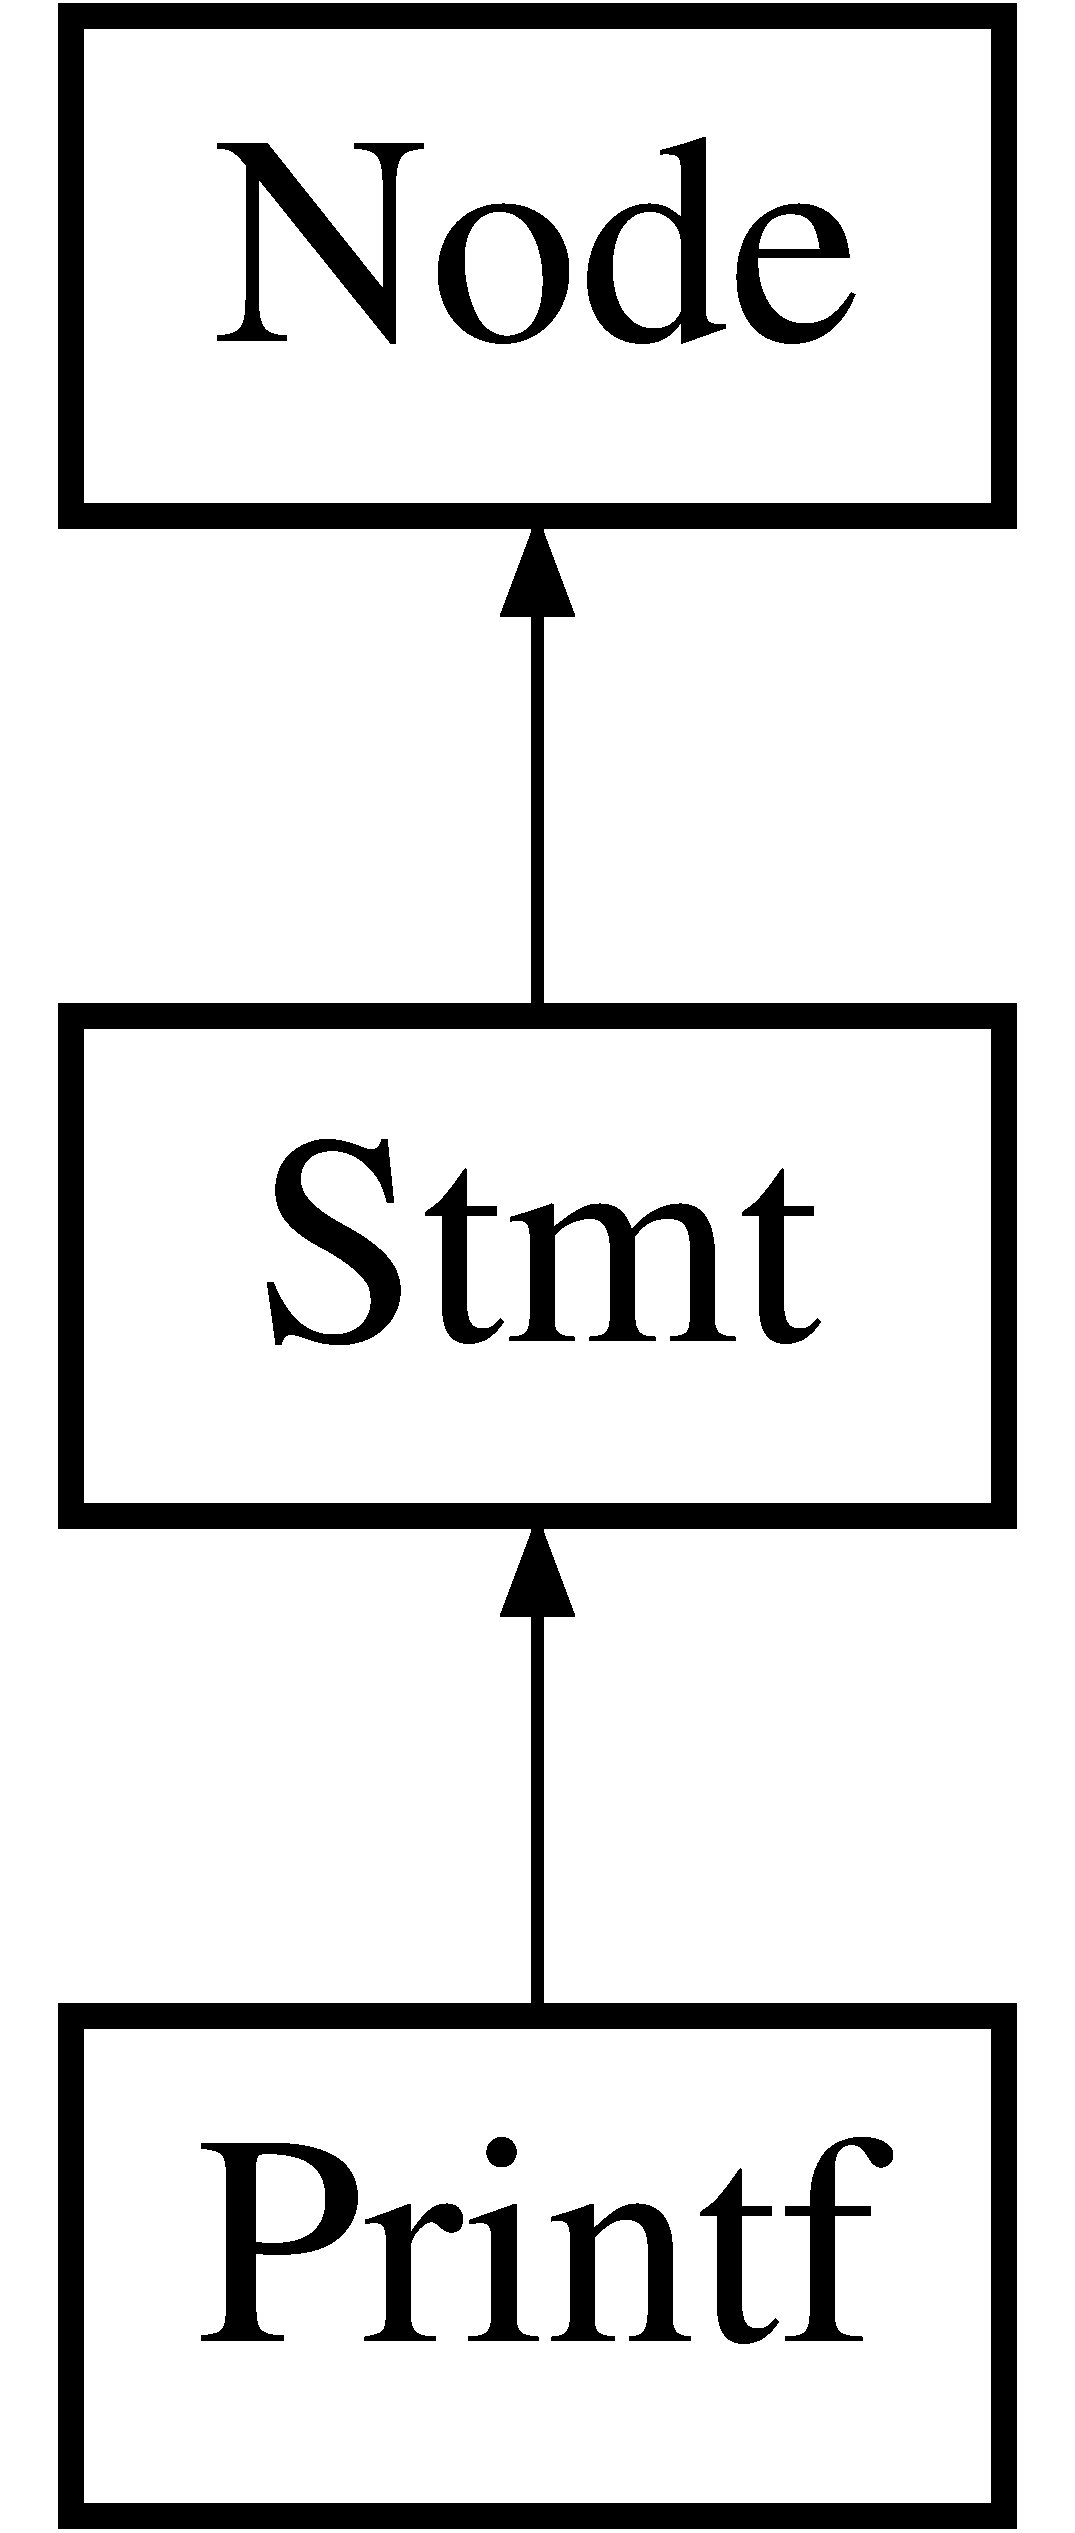
\includegraphics[height=3.000000cm]{class_printf}
\end{center}
\end{figure}
\subsection*{Public Member Functions}
\begin{DoxyCompactItemize}
\item 
int \hyperlink{class_printf_a0343199e28647ced40b9d74a284ff5f3}{execute} ()
\begin{DoxyCompactList}\small\item\em 抽象的执行方法 \end{DoxyCompactList}\end{DoxyCompactItemize}
\subsection*{Public Attributes}
\begin{DoxyCompactItemize}
\item 
std\+::vector$<$ \hyperlink{class_expr}{Expr} $\ast$ $>$ \hyperlink{class_printf_ab07a181eb9cd79c9018e172332d44ce5}{exprs}
\end{DoxyCompactItemize}
\subsection*{Additional Inherited Members}


\subsection{Member Function Documentation}
\mbox{\Hypertarget{class_printf_a0343199e28647ced40b9d74a284ff5f3}\label{class_printf_a0343199e28647ced40b9d74a284ff5f3}} 
\index{Printf@{Printf}!execute@{execute}}
\index{execute@{execute}!Printf@{Printf}}
\subsubsection{\texorpdfstring{execute()}{execute()}}
{\footnotesize\ttfamily int Printf\+::execute (\begin{DoxyParamCaption}{ }\end{DoxyParamCaption})\hspace{0.3cm}{\ttfamily [virtual]}}



抽象的执行方法 

因为表达式以及各种语句都是可执行的~\newline
设立这个方法利用多态可以实现整个语法树的执行~\newline
 \begin{DoxyReturn}{Returns}
int \+: 表达式或语句执行后获得的值 
\end{DoxyReturn}


Reimplemented from \hyperlink{class_stmt_abdc3261770c3c5bd3ce5b3ba6eedfaa4}{Stmt}.



\subsection{Member Data Documentation}
\mbox{\Hypertarget{class_printf_ab07a181eb9cd79c9018e172332d44ce5}\label{class_printf_ab07a181eb9cd79c9018e172332d44ce5}} 
\index{Printf@{Printf}!exprs@{exprs}}
\index{exprs@{exprs}!Printf@{Printf}}
\subsubsection{\texorpdfstring{exprs}{exprs}}
{\footnotesize\ttfamily std\+::vector$<$\hyperlink{class_expr}{Expr}$\ast$$>$ Printf\+::exprs}



The documentation for this class was generated from the following files\+:\begin{DoxyCompactItemize}
\item 
src/inter/stmt/\hyperlink{_printf_8h}{Printf.\+h}\item 
src/inter/stmt/\hyperlink{_printf_8cpp}{Printf.\+cpp}\end{DoxyCompactItemize}

\hypertarget{class_rel}{}\section{Rel Class Reference}
\label{class_rel}\index{Rel@{Rel}}


大小于运算符类  




{\ttfamily \#include $<$Rel.\+h$>$}

Inheritance diagram for Rel\+:\begin{figure}[H]
\begin{center}
\leavevmode
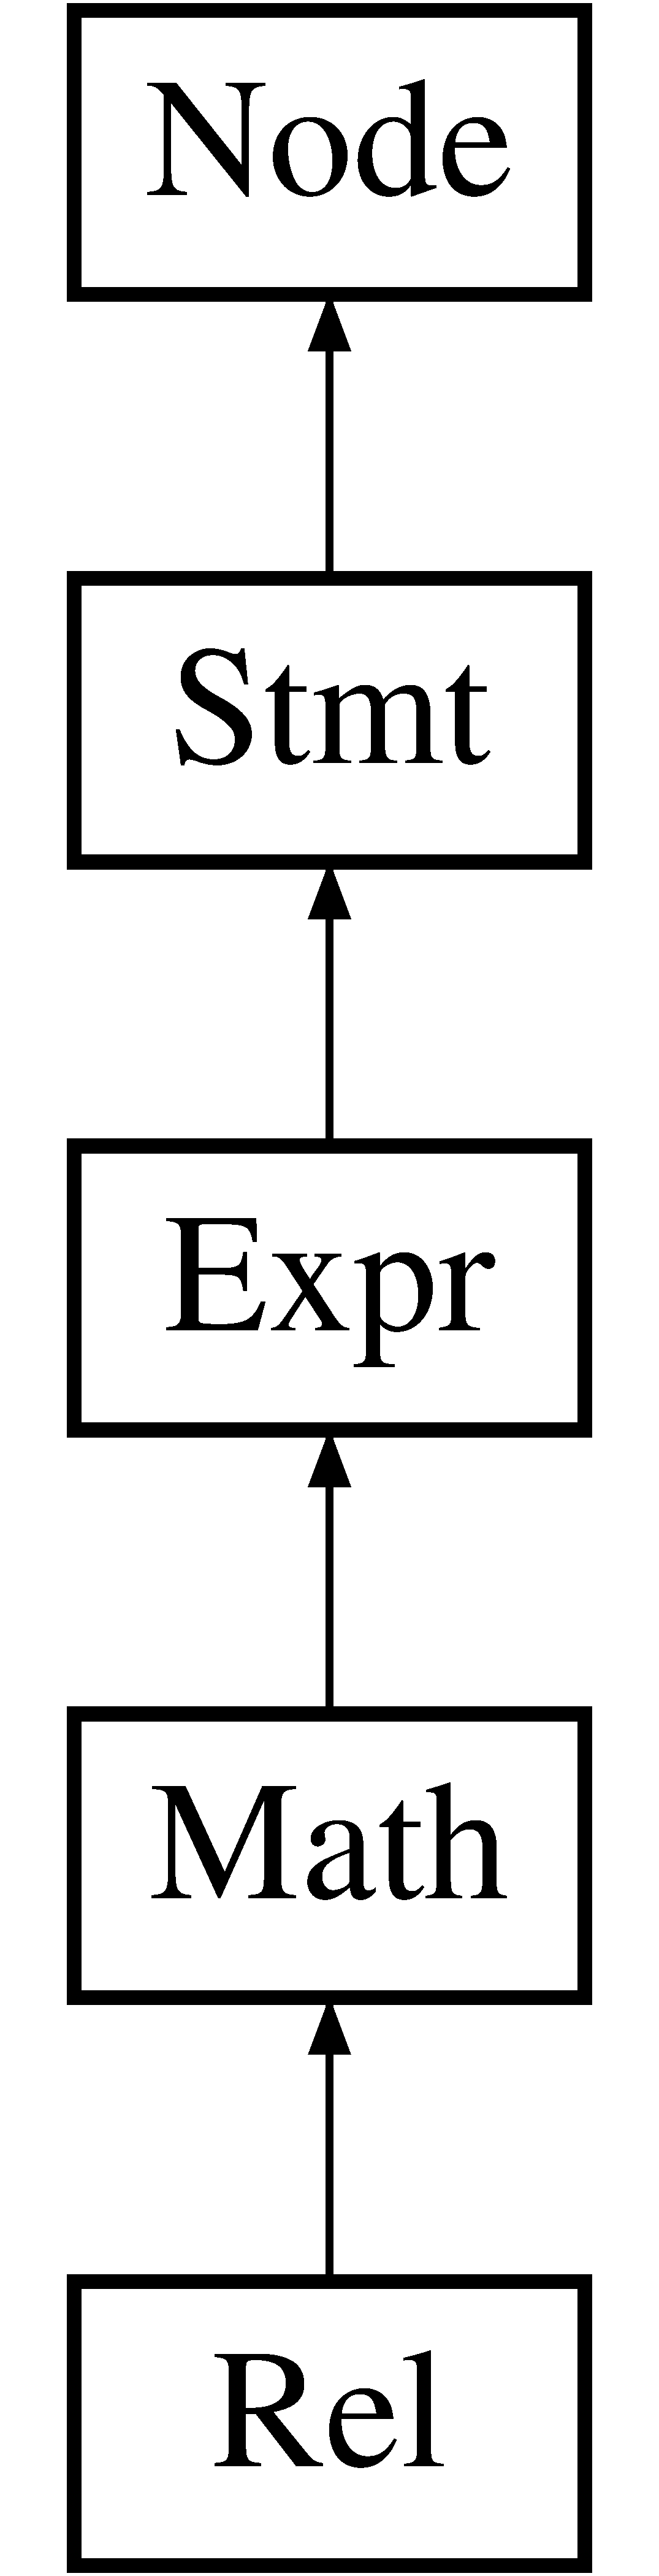
\includegraphics[height=5.000000cm]{class_rel}
\end{center}
\end{figure}
\subsection*{Public Member Functions}
\begin{DoxyCompactItemize}
\item 
\hyperlink{class_rel_a1f60bc90adde19ed35f26ea8b2cfd91c}{Rel} (\hyperlink{class_token}{Token} $\ast$token, \hyperlink{class_expr}{Expr} $\ast$expr1, \hyperlink{class_expr}{Expr} $\ast$expr2)
\item 
\mbox{\Hypertarget{class_rel_a82b2f3b75a2b9e81631f2659d42a36d1}\label{class_rel_a82b2f3b75a2b9e81631f2659d42a36d1}} 
int \hyperlink{class_rel_a82b2f3b75a2b9e81631f2659d42a36d1}{execute} ()
\begin{DoxyCompactList}\small\item\em 返回复制后的变量 \end{DoxyCompactList}\end{DoxyCompactItemize}
\subsection*{Additional Inherited Members}


\subsection{Detailed Description}
大小于运算符类 

\subsection{Constructor \& Destructor Documentation}
\mbox{\Hypertarget{class_rel_a1f60bc90adde19ed35f26ea8b2cfd91c}\label{class_rel_a1f60bc90adde19ed35f26ea8b2cfd91c}} 
\index{Rel@{Rel}!Rel@{Rel}}
\index{Rel@{Rel}!Rel@{Rel}}
\subsubsection{\texorpdfstring{Rel()}{Rel()}}
{\footnotesize\ttfamily Rel\+::\+Rel (\begin{DoxyParamCaption}\item[{\hyperlink{class_token}{Token} $\ast$}]{token,  }\item[{\hyperlink{class_expr}{Expr} $\ast$}]{expr1,  }\item[{\hyperlink{class_expr}{Expr} $\ast$}]{expr2 }\end{DoxyParamCaption})}


\begin{DoxyParams}{Parameters}
{\em token} & \+: 运算符 \\
\hline
{\em expr1} & \+: 左表达式 \\
\hline
{\em expr2} & \+: 右表达式 \\
\hline
\end{DoxyParams}


The documentation for this class was generated from the following files\+:\begin{DoxyCompactItemize}
\item 
src/inter/stmt/expr/Rel.\+h\item 
src/inter/stmt/expr/Rel.\+cpp\end{DoxyCompactItemize}

\hypertarget{class_self_op}{}\section{Self\+Op类 参考}
\label{class_self_op}\index{Self\+Op@{Self\+Op}}


赋值运算符类  




{\ttfamily \#include $<$Self\+Op.\+h$>$}

类 Self\+Op 继承关系图\+:\begin{figure}[H]
\begin{center}
\leavevmode
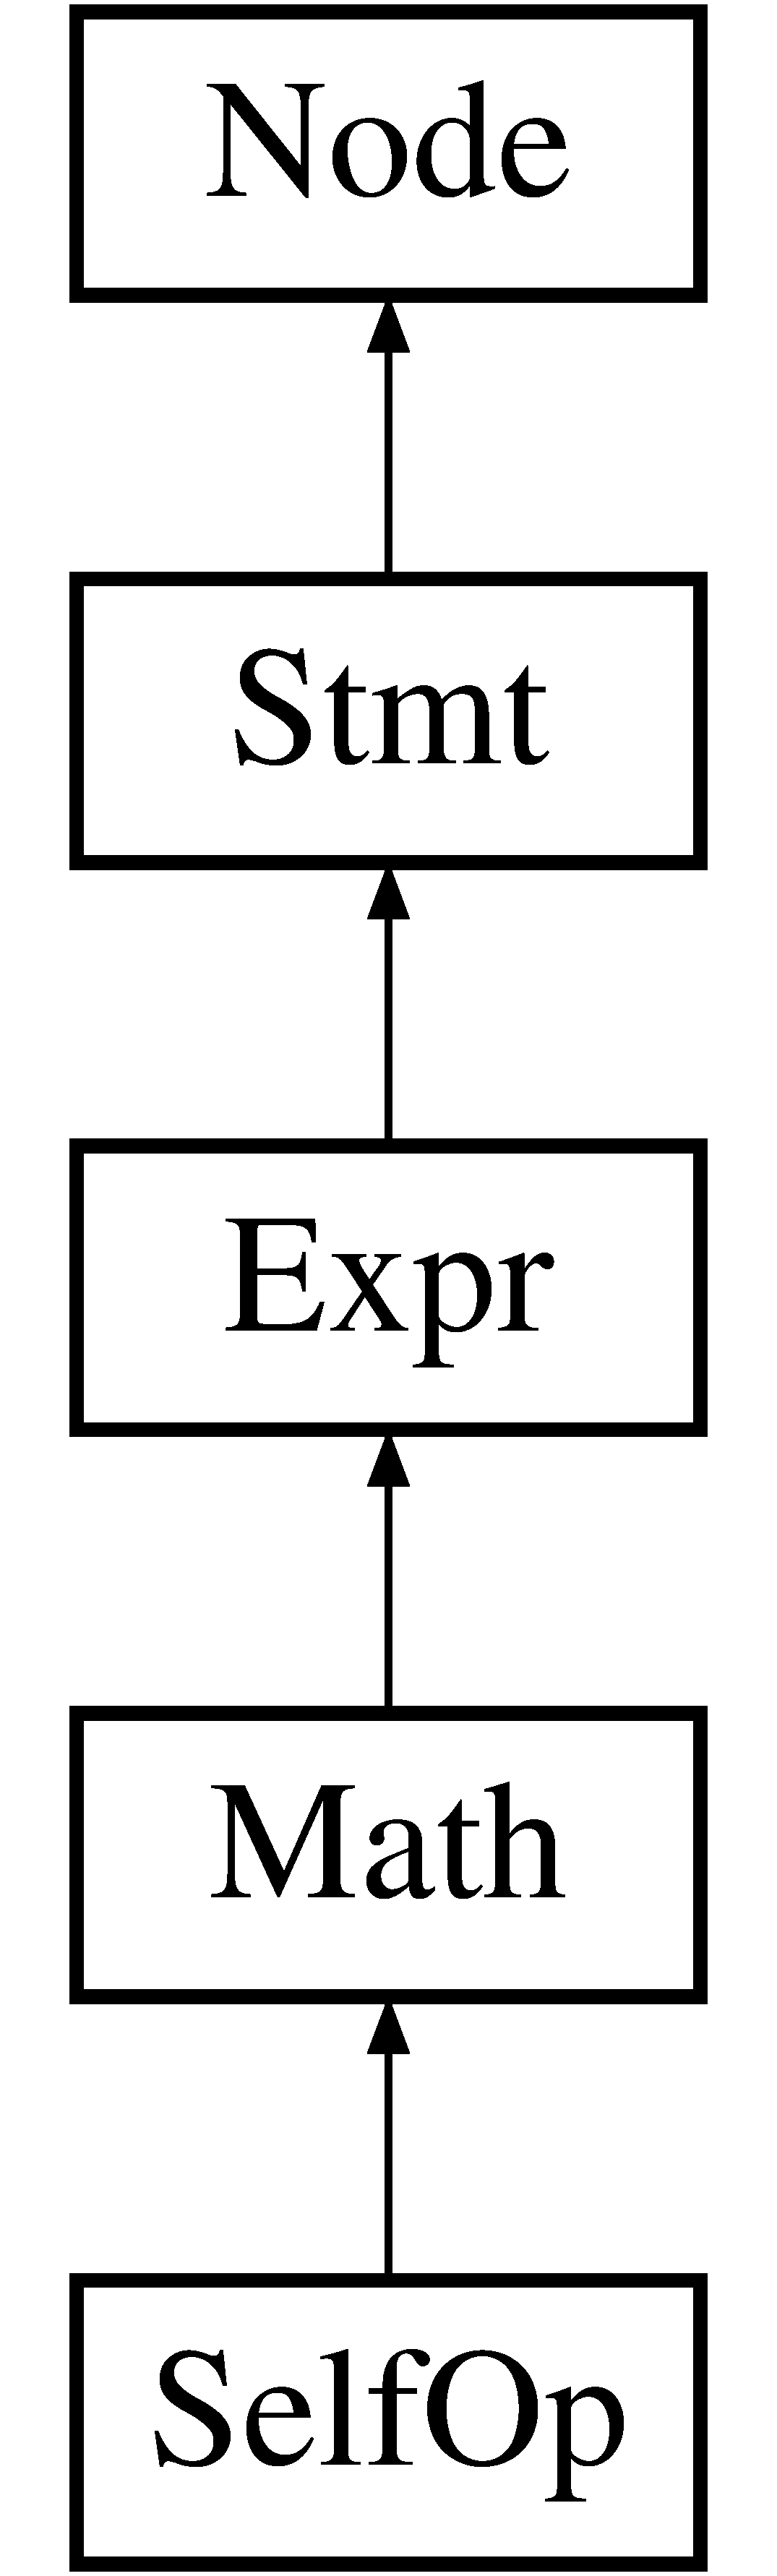
\includegraphics[height=5.000000cm]{class_self_op}
\end{center}
\end{figure}
\subsection*{Public 成员函数}
\begin{DoxyCompactItemize}
\item 
\hyperlink{class_self_op_a5292e81fca1817185db15b29564a32ee}{Self\+Op} (\hyperlink{class_token}{Token} $\ast$token, \hyperlink{class_expr}{Expr} $\ast$expr)
\item 
\mbox{\Hypertarget{class_self_op_ab452bcad1cd4f1286813b1f737583818}\label{class_self_op_ab452bcad1cd4f1286813b1f737583818}} 
int \hyperlink{class_self_op_ab452bcad1cd4f1286813b1f737583818}{execute} ()
\begin{DoxyCompactList}\small\item\em 返回复制后的变量值 \end{DoxyCompactList}\end{DoxyCompactItemize}
\subsection*{额外继承的成员函数}


\subsection{详细描述}
赋值运算符类 

\subsection{构造及析构函数说明}
\mbox{\Hypertarget{class_self_op_a5292e81fca1817185db15b29564a32ee}\label{class_self_op_a5292e81fca1817185db15b29564a32ee}} 
\index{Self\+Op@{Self\+Op}!Self\+Op@{Self\+Op}}
\index{Self\+Op@{Self\+Op}!Self\+Op@{Self\+Op}}
\subsubsection{\texorpdfstring{Self\+Op()}{SelfOp()}}
{\footnotesize\ttfamily Self\+Op\+::\+Self\+Op (\begin{DoxyParamCaption}\item[{\hyperlink{class_token}{Token} $\ast$}]{token,  }\item[{\hyperlink{class_expr}{Expr} $\ast$}]{expr }\end{DoxyParamCaption})}


\begin{DoxyParams}{参数}
{\em token} & \+: 运算符 \\
\hline
{\em expr} & \+: 表达式 \\
\hline
\end{DoxyParams}


该类的文档由以下文件生成\+:\begin{DoxyCompactItemize}
\item 
src/inter/stmt/expr/Self\+Op.\+h\item 
src/inter/stmt/expr/Self\+Op.\+cpp\end{DoxyCompactItemize}

\hypertarget{class_set}{}\section{Set类 参考}
\label{class_set}\index{Set@{Set}}


赋值运算符类  




{\ttfamily \#include $<$Set.\+h$>$}

类 Set 继承关系图\+:\begin{figure}[H]
\begin{center}
\leavevmode
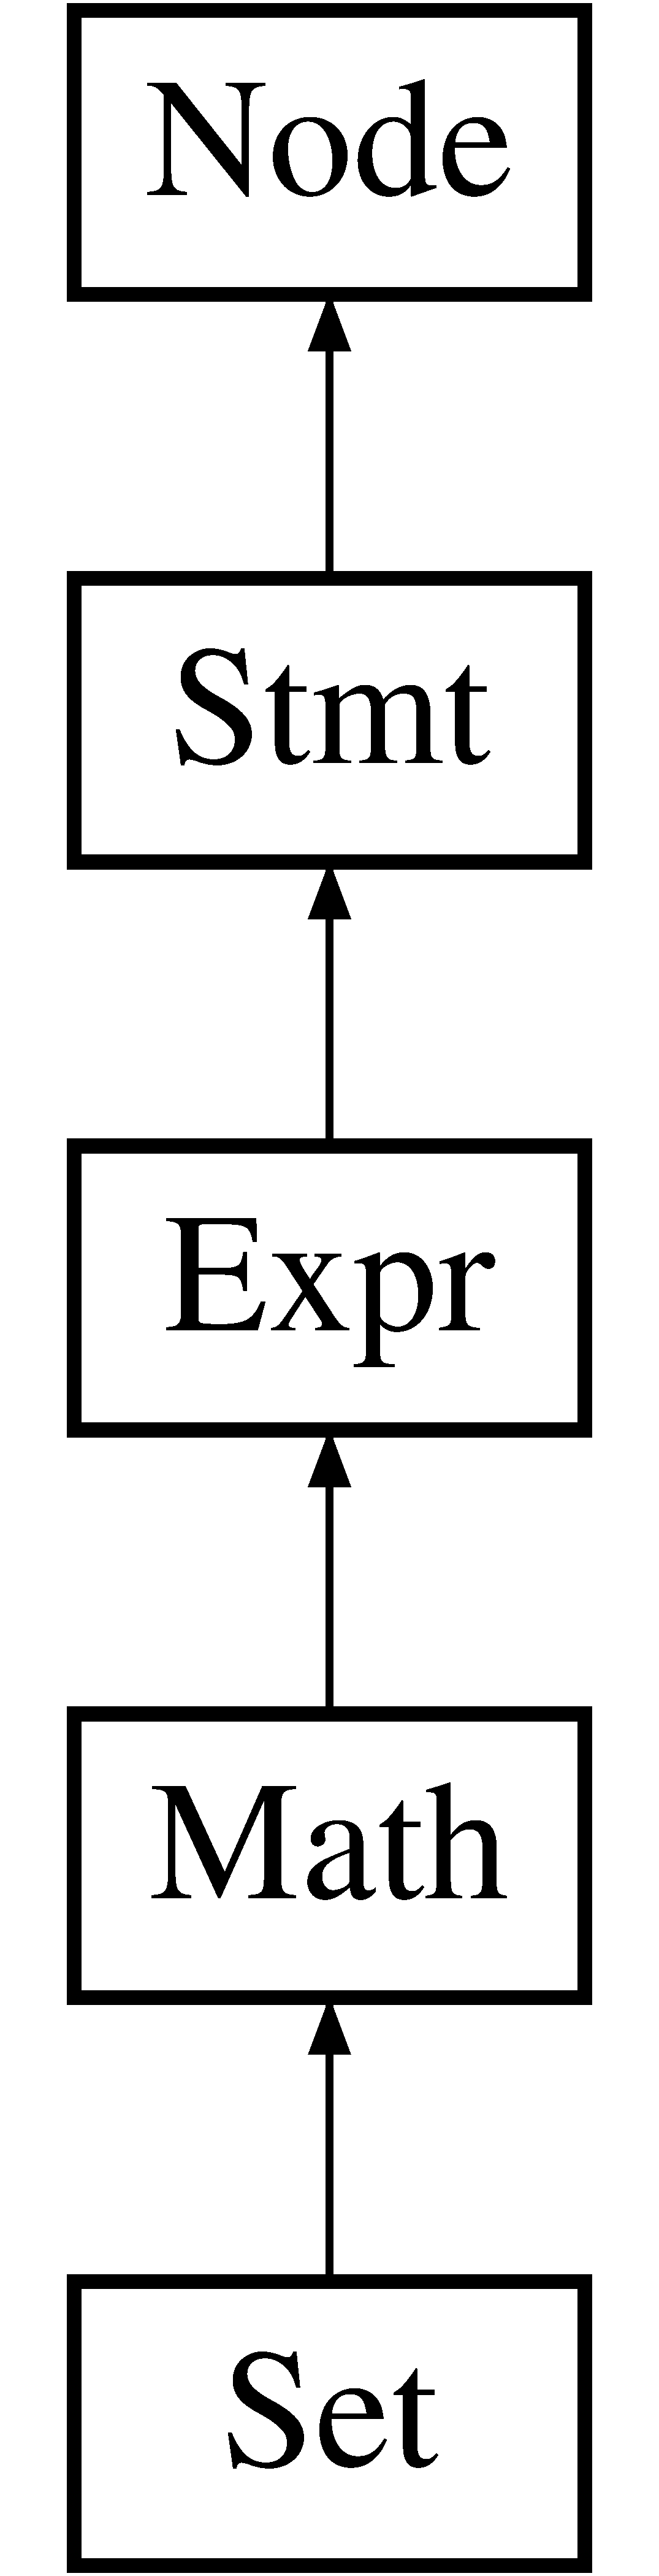
\includegraphics[height=5.000000cm]{class_set}
\end{center}
\end{figure}
\subsection*{Public 成员函数}
\begin{DoxyCompactItemize}
\item 
\hyperlink{class_set_a05474c6de277894bcebe5230c587efab}{Set} (\hyperlink{class_token}{Token} $\ast$token, \hyperlink{class_var}{Var} $\ast$var, \hyperlink{class_expr}{Expr} $\ast$expr)
\item 
int \hyperlink{class_set_a7776ba36f3af8b09772b36927beb5f5c}{execute} ()\hypertarget{class_set_a7776ba36f3af8b09772b36927beb5f5c}{}\label{class_set_a7776ba36f3af8b09772b36927beb5f5c}

\begin{DoxyCompactList}\small\item\em 返回复制后的变量值 \end{DoxyCompactList}\end{DoxyCompactItemize}
\subsection*{额外继承的成员函数}


\subsection{详细描述}
赋值运算符类 

\subsection{构造及析构函数说明}
\index{Set@{Set}!Set@{Set}}
\index{Set@{Set}!Set@{Set}}
\subsubsection[{\texorpdfstring{Set(\+Token $\ast$token, Var $\ast$var, Expr $\ast$expr)}{Set(Token *token, Var *var, Expr *expr)}}]{\setlength{\rightskip}{0pt plus 5cm}Set\+::\+Set (
\begin{DoxyParamCaption}
\item[{{\bf Token} $\ast$}]{token, }
\item[{{\bf Var} $\ast$}]{var, }
\item[{{\bf Expr} $\ast$}]{expr}
\end{DoxyParamCaption}
)}\hypertarget{class_set_a05474c6de277894bcebe5230c587efab}{}\label{class_set_a05474c6de277894bcebe5230c587efab}

\begin{DoxyParams}{参数}
{\em token} & \+: 运算符 \\
\hline
{\em var} & \+: 变量 \\
\hline
{\em expr} & \+: 右表达式 \\
\hline
\end{DoxyParams}


该类的文档由以下文件生成\+:\begin{DoxyCompactItemize}
\item 
src/inter/stmt/expr/Set.\+h\item 
src/inter/stmt/expr/Set.\+cpp\end{DoxyCompactItemize}

\hypertarget{class_stmt}{}\section{Stmt Class Reference}
\label{class_stmt}\index{Stmt@{Stmt}}


Stmt类  




{\ttfamily \#include $<$Stmt.\+h$>$}

Inheritance diagram for Stmt\+:\begin{figure}[H]
\begin{center}
\leavevmode
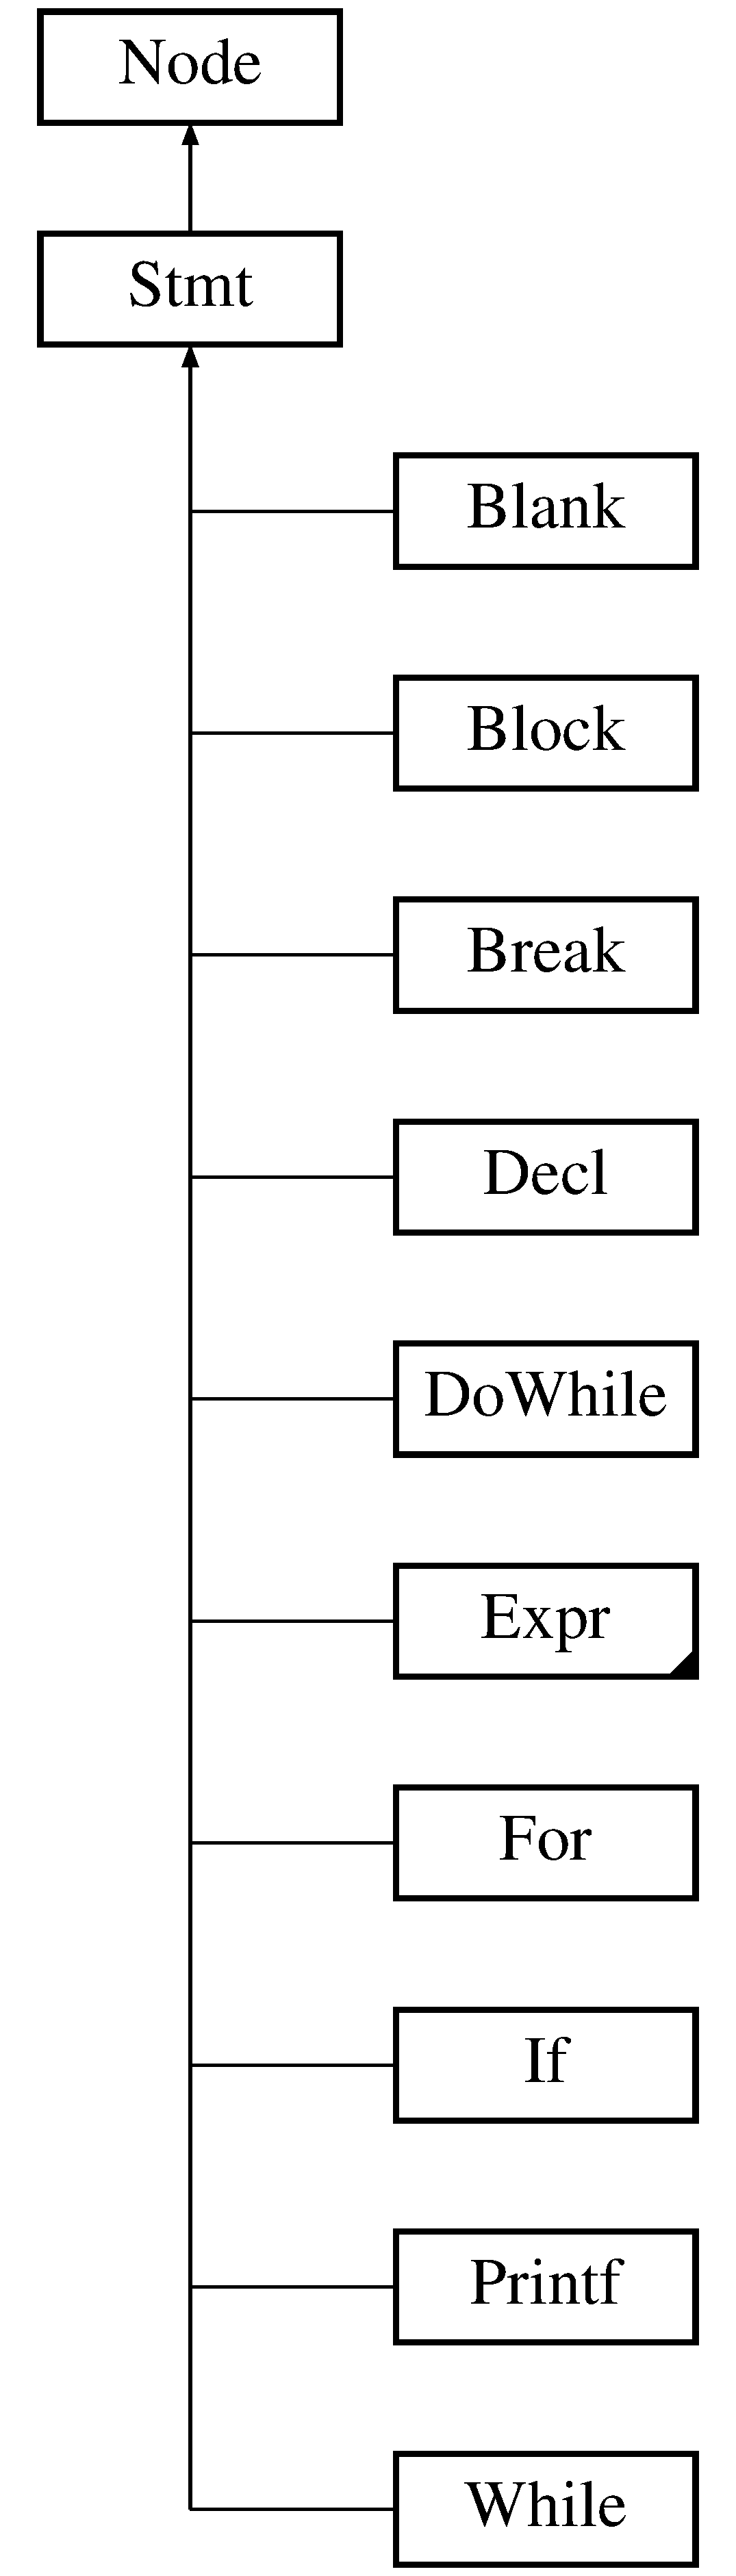
\includegraphics[height=12.000000cm]{class_stmt}
\end{center}
\end{figure}
\subsection*{Public Member Functions}
\begin{DoxyCompactItemize}
\item 
virtual int \hyperlink{class_stmt_abdc3261770c3c5bd3ce5b3ba6eedfaa4}{execute} ()
\begin{DoxyCompactList}\small\item\em 抽象的执行方法 \end{DoxyCompactList}\end{DoxyCompactItemize}
\subsection*{Additional Inherited Members}


\subsection{Detailed Description}
Stmt类 

所有语句,表达式的超类~\newline
定义语句基本的行为 

\subsection{Member Function Documentation}
\mbox{\Hypertarget{class_stmt_abdc3261770c3c5bd3ce5b3ba6eedfaa4}\label{class_stmt_abdc3261770c3c5bd3ce5b3ba6eedfaa4}} 
\index{Stmt@{Stmt}!execute@{execute}}
\index{execute@{execute}!Stmt@{Stmt}}
\subsubsection{\texorpdfstring{execute()}{execute()}}
{\footnotesize\ttfamily int Stmt\+::execute (\begin{DoxyParamCaption}{ }\end{DoxyParamCaption})\hspace{0.3cm}{\ttfamily [virtual]}}



抽象的执行方法 

因为表达式以及各种语句都是可执行的~\newline
设立这个方法利用多态可以实现整个语法树的执行~\newline
 \begin{DoxyReturn}{Returns}
int \+: 表达式或语句执行后获得的值 
\end{DoxyReturn}


Reimplemented in \hyperlink{class_var_a9dc96e803f7b0f9aa519c2c0e0a6bd8f}{Var}, \hyperlink{class_set_a7776ba36f3af8b09772b36927beb5f5c}{Set}, \hyperlink{class_block_a8e03f15df4e43cd6c802341c3bda6b33}{Block}, \hyperlink{class_unary_af42edff1ee4718a9afeb7127e41af758}{Unary}, \hyperlink{class_comma_aab9ca2bb70a10abd2fb263de745f843a}{Comma}, \hyperlink{class_equality_a0255c33af70613b006b03a329ed329ff}{Equality}, \hyperlink{class_term_ac2d20115da73f9425e5d390856a211a1}{Term}, \hyperlink{class_for_ad099d6d48c640dd5127285e59bbaba15}{For}, \hyperlink{class_if_aeadf929258ccd07a239879c118fb152f}{If}, \hyperlink{class_rel_a82b2f3b75a2b9e81631f2659d42a36d1}{Rel}, \hyperlink{class_self_op_ab452bcad1cd4f1286813b1f737583818}{Self\+Op}, \hyperlink{class_add_sub_a73c0513a31a5400fdfc79ce877a1c3b9}{Add\+Sub}, \hyperlink{class_expr_aff6a2e6eaa460e2a3db28ebdab089b51}{Expr}, \hyperlink{class_id_ae43a9ffecbbc0ac4fd041b8e8e3c3de0}{Id}, \hyperlink{class_decl_ad6495a4245a45dcdcd05e239c8db4a8b}{Decl}, \hyperlink{class_constant_ab5c55607bcff5ce70131a588b6bdbed7}{Constant}, \hyperlink{class_printf_a0343199e28647ced40b9d74a284ff5f3}{Printf}, \hyperlink{class_while_a23b58565983130bb54577f4399ffd822}{While}, \hyperlink{class_do_while_adb6934e033f44c6b52b1079faf1d84cf}{Do\+While}, and \hyperlink{class_break_a554fd4cae05d203145d62868f73004d4}{Break}.



The documentation for this class was generated from the following files\+:\begin{DoxyCompactItemize}
\item 
src/inter/stmt/Stmt.\+h\item 
src/inter/stmt/Stmt.\+cpp\end{DoxyCompactItemize}

\hypertarget{class_syntax_error}{}\section{Syntax\+Error Class Reference}
\label{class_syntax_error}\index{Syntax\+Error@{Syntax\+Error}}


语法错误类  




{\ttfamily \#include $<$Syntax\+Error.\+h$>$}

Inheritance diagram for Syntax\+Error\+:\begin{figure}[H]
\begin{center}
\leavevmode
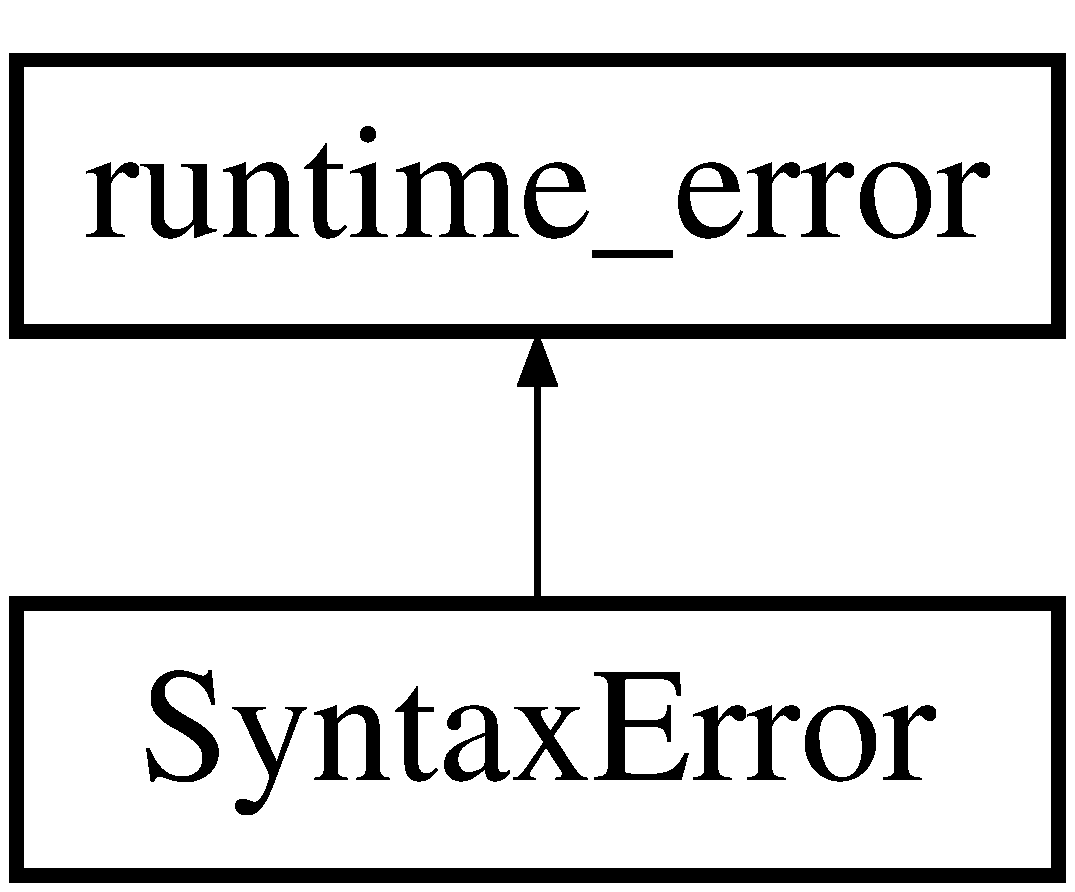
\includegraphics[height=2.000000cm]{class_syntax_error}
\end{center}
\end{figure}
\subsection*{Public Member Functions}
\begin{DoxyCompactItemize}
\item 
\mbox{\Hypertarget{class_syntax_error_a41285cf1cafd071040aec4382e0d7dcd}\label{class_syntax_error_a41285cf1cafd071040aec4382e0d7dcd}} 
{\bfseries Syntax\+Error} (std\+::string)
\end{DoxyCompactItemize}


\subsection{Detailed Description}
语法错误类 

在语法分析时, 若是匹配项与语法不一致时 就会抛出此错误 

The documentation for this class was generated from the following files\+:\begin{DoxyCompactItemize}
\item 
src/parser/Syntax\+Error.\+h\item 
src/parser/Syntax\+Error.\+cpp\end{DoxyCompactItemize}

\hypertarget{class_tag}{}\section{Tag Class Reference}
\label{class_tag}\index{Tag@{Tag}}


{\ttfamily \#include $<$Tag.\+h$>$}

\subsection*{Static Public Attributes}
\begin{DoxyCompactItemize}
\item 
static const int \hyperlink{class_tag_acdf9d38c11c7dff1026caea53454d62c}{ID} = 256
\item 
static const int \hyperlink{class_tag_a37bd7cc8cc362fca325f553b2844d745}{N\+UM} = 257
\item 
static const int \hyperlink{class_tag_a383b3b3d27ad94992a9345cf51632f31}{Semicolon} = \textquotesingle{};\textquotesingle{}
\item 
static const int \hyperlink{class_tag_a3f592bff8a566859e6953cd380e809e7}{L\+\_\+\+P\+A\+R\+E\+N\+T\+H\+E\+SE} = \textquotesingle{}(\textquotesingle{}
\item 
static const int \hyperlink{class_tag_a06f70b28d8eb3e9f3d2d7dcc6a318fee}{R\+\_\+\+P\+A\+R\+E\+N\+T\+H\+E\+SE} = \textquotesingle{})\textquotesingle{}
\item 
static const int \hyperlink{class_tag_a27f8b6e653f63d5a04cbf773d7aef40d}{L\+\_\+\+B\+R\+A\+CE} = \textquotesingle{}\{\textquotesingle{}
\item 
static const int \hyperlink{class_tag_ac75cf51168e5f889ec56a8e5cebc4483}{R\+\_\+\+B\+R\+A\+CE} = \textquotesingle{}\}\textquotesingle{}
\item 
static const int \hyperlink{class_tag_ad0218cdf6f9bc11b27aa07dc789e0a2c}{C\+O\+M\+MA} = \textquotesingle{},\textquotesingle{}
\item 
static const int \hyperlink{class_tag_aa94fc1145460d63eb408321dd9b2b4c6}{P\+L\+US} = \textquotesingle{}+\textquotesingle{}
\item 
static const int \hyperlink{class_tag_a74a3061b0a3125dae8759a9490298b28}{S\+UB} = \textquotesingle{}-\/\textquotesingle{}
\item 
static const int \hyperlink{class_tag_a2adc4fe55411d9f65477992a527601fe}{M\+U\+LT} = \textquotesingle{}$\ast$\textquotesingle{}
\item 
static const int \hyperlink{class_tag_a17b55c27354f38f161e670ca29e26ce0}{D\+IV} = \textquotesingle{}/\textquotesingle{}
\item 
static const int \hyperlink{class_tag_aaad09d061ef5a1979f0742f3df402cc0}{LT} = \textquotesingle{}$<$\textquotesingle{}
\item 
static const int \hyperlink{class_tag_a6805be845a48a88f70bec57afd269c95}{GT} = \textquotesingle{}$>$\textquotesingle{}
\item 
static const int \hyperlink{class_tag_a6d994a4cb6c7fcb155a03b7a91d44bcb}{GE} = 264
\item 
static const int \hyperlink{class_tag_adc918b8b4103c25ea473e7b15bb7bab9}{LE} = 265
\item 
static const int \hyperlink{class_tag_adaaf58a2112230b36e757ef7c70d6fe9}{NE} = 266
\item 
static const int \hyperlink{class_tag_a654bec3c95903280d16610fadf8eeec5}{EQ} = 267
\item 
static const int \hyperlink{class_tag_aed087674890e23fb6678d597824c2613}{I\+N\+C\+RE} = 268
\item 
static const int \hyperlink{class_tag_ab37502d40b1d318449f44302ff5db17d}{D\+E\+C\+RE} = 269
\item 
static const int \hyperlink{class_tag_a38242d609491f491ef9484f1679e7c3d}{I\+NT} = 258
\item 
static const int \hyperlink{class_tag_a92a30db62631be16cad518d2bf59efaa}{IF} = 259
\item 
static const int \hyperlink{class_tag_a4149b756bf94ef2d83f0d1de23ddee10}{E\+L\+SE} = 260
\item 
static const int \hyperlink{class_tag_ac2ba80666f85af3bd539107c7121b16d}{F\+OR} = 261
\item 
static const int \hyperlink{class_tag_a489769ae22c0fcf7c7842206a998abf8}{DO} = 262
\item 
static const int \hyperlink{class_tag_a1ca35b43b49867c19d892103016b09b3}{W\+H\+I\+LE} = 263
\item 
static const int \hyperlink{class_tag_a125fe413cdcec181606fa122a40f0026}{B\+R\+E\+AK} = 270
\item 
static const int \hyperlink{class_tag_a85ff0086e29d3d6a8f6c78695df0bd52}{P\+R\+I\+N\+TF} = 271
\end{DoxyCompactItemize}


\subsection{Member Data Documentation}
\mbox{\Hypertarget{class_tag_a125fe413cdcec181606fa122a40f0026}\label{class_tag_a125fe413cdcec181606fa122a40f0026}} 
\index{Tag@{Tag}!B\+R\+E\+AK@{B\+R\+E\+AK}}
\index{B\+R\+E\+AK@{B\+R\+E\+AK}!Tag@{Tag}}
\subsubsection{\texorpdfstring{B\+R\+E\+AK}{BREAK}}
{\footnotesize\ttfamily const int Tag\+::\+B\+R\+E\+AK = 270\hspace{0.3cm}{\ttfamily [static]}}

\mbox{\Hypertarget{class_tag_ad0218cdf6f9bc11b27aa07dc789e0a2c}\label{class_tag_ad0218cdf6f9bc11b27aa07dc789e0a2c}} 
\index{Tag@{Tag}!C\+O\+M\+MA@{C\+O\+M\+MA}}
\index{C\+O\+M\+MA@{C\+O\+M\+MA}!Tag@{Tag}}
\subsubsection{\texorpdfstring{C\+O\+M\+MA}{COMMA}}
{\footnotesize\ttfamily const int Tag\+::\+C\+O\+M\+MA = \textquotesingle{},\textquotesingle{}\hspace{0.3cm}{\ttfamily [static]}}

\mbox{\Hypertarget{class_tag_ab37502d40b1d318449f44302ff5db17d}\label{class_tag_ab37502d40b1d318449f44302ff5db17d}} 
\index{Tag@{Tag}!D\+E\+C\+RE@{D\+E\+C\+RE}}
\index{D\+E\+C\+RE@{D\+E\+C\+RE}!Tag@{Tag}}
\subsubsection{\texorpdfstring{D\+E\+C\+RE}{DECRE}}
{\footnotesize\ttfamily const int Tag\+::\+D\+E\+C\+RE = 269\hspace{0.3cm}{\ttfamily [static]}}

\mbox{\Hypertarget{class_tag_a17b55c27354f38f161e670ca29e26ce0}\label{class_tag_a17b55c27354f38f161e670ca29e26ce0}} 
\index{Tag@{Tag}!D\+IV@{D\+IV}}
\index{D\+IV@{D\+IV}!Tag@{Tag}}
\subsubsection{\texorpdfstring{D\+IV}{DIV}}
{\footnotesize\ttfamily const int Tag\+::\+D\+IV = \textquotesingle{}/\textquotesingle{}\hspace{0.3cm}{\ttfamily [static]}}

\mbox{\Hypertarget{class_tag_a489769ae22c0fcf7c7842206a998abf8}\label{class_tag_a489769ae22c0fcf7c7842206a998abf8}} 
\index{Tag@{Tag}!DO@{DO}}
\index{DO@{DO}!Tag@{Tag}}
\subsubsection{\texorpdfstring{DO}{DO}}
{\footnotesize\ttfamily const int Tag\+::\+DO = 262\hspace{0.3cm}{\ttfamily [static]}}

\mbox{\Hypertarget{class_tag_a4149b756bf94ef2d83f0d1de23ddee10}\label{class_tag_a4149b756bf94ef2d83f0d1de23ddee10}} 
\index{Tag@{Tag}!E\+L\+SE@{E\+L\+SE}}
\index{E\+L\+SE@{E\+L\+SE}!Tag@{Tag}}
\subsubsection{\texorpdfstring{E\+L\+SE}{ELSE}}
{\footnotesize\ttfamily const int Tag\+::\+E\+L\+SE = 260\hspace{0.3cm}{\ttfamily [static]}}

\mbox{\Hypertarget{class_tag_a654bec3c95903280d16610fadf8eeec5}\label{class_tag_a654bec3c95903280d16610fadf8eeec5}} 
\index{Tag@{Tag}!EQ@{EQ}}
\index{EQ@{EQ}!Tag@{Tag}}
\subsubsection{\texorpdfstring{EQ}{EQ}}
{\footnotesize\ttfamily const int Tag\+::\+EQ = 267\hspace{0.3cm}{\ttfamily [static]}}

\mbox{\Hypertarget{class_tag_ac2ba80666f85af3bd539107c7121b16d}\label{class_tag_ac2ba80666f85af3bd539107c7121b16d}} 
\index{Tag@{Tag}!F\+OR@{F\+OR}}
\index{F\+OR@{F\+OR}!Tag@{Tag}}
\subsubsection{\texorpdfstring{F\+OR}{FOR}}
{\footnotesize\ttfamily const int Tag\+::\+F\+OR = 261\hspace{0.3cm}{\ttfamily [static]}}

\mbox{\Hypertarget{class_tag_a6d994a4cb6c7fcb155a03b7a91d44bcb}\label{class_tag_a6d994a4cb6c7fcb155a03b7a91d44bcb}} 
\index{Tag@{Tag}!GE@{GE}}
\index{GE@{GE}!Tag@{Tag}}
\subsubsection{\texorpdfstring{GE}{GE}}
{\footnotesize\ttfamily const int Tag\+::\+GE = 264\hspace{0.3cm}{\ttfamily [static]}}

\mbox{\Hypertarget{class_tag_a6805be845a48a88f70bec57afd269c95}\label{class_tag_a6805be845a48a88f70bec57afd269c95}} 
\index{Tag@{Tag}!GT@{GT}}
\index{GT@{GT}!Tag@{Tag}}
\subsubsection{\texorpdfstring{GT}{GT}}
{\footnotesize\ttfamily const int Tag\+::\+GT = \textquotesingle{}$>$\textquotesingle{}\hspace{0.3cm}{\ttfamily [static]}}

\mbox{\Hypertarget{class_tag_acdf9d38c11c7dff1026caea53454d62c}\label{class_tag_acdf9d38c11c7dff1026caea53454d62c}} 
\index{Tag@{Tag}!ID@{ID}}
\index{ID@{ID}!Tag@{Tag}}
\subsubsection{\texorpdfstring{ID}{ID}}
{\footnotesize\ttfamily const int Tag\+::\+ID = 256\hspace{0.3cm}{\ttfamily [static]}}

\mbox{\Hypertarget{class_tag_a92a30db62631be16cad518d2bf59efaa}\label{class_tag_a92a30db62631be16cad518d2bf59efaa}} 
\index{Tag@{Tag}!IF@{IF}}
\index{IF@{IF}!Tag@{Tag}}
\subsubsection{\texorpdfstring{IF}{IF}}
{\footnotesize\ttfamily const int Tag\+::\+IF = 259\hspace{0.3cm}{\ttfamily [static]}}

\mbox{\Hypertarget{class_tag_aed087674890e23fb6678d597824c2613}\label{class_tag_aed087674890e23fb6678d597824c2613}} 
\index{Tag@{Tag}!I\+N\+C\+RE@{I\+N\+C\+RE}}
\index{I\+N\+C\+RE@{I\+N\+C\+RE}!Tag@{Tag}}
\subsubsection{\texorpdfstring{I\+N\+C\+RE}{INCRE}}
{\footnotesize\ttfamily const int Tag\+::\+I\+N\+C\+RE = 268\hspace{0.3cm}{\ttfamily [static]}}

\mbox{\Hypertarget{class_tag_a38242d609491f491ef9484f1679e7c3d}\label{class_tag_a38242d609491f491ef9484f1679e7c3d}} 
\index{Tag@{Tag}!I\+NT@{I\+NT}}
\index{I\+NT@{I\+NT}!Tag@{Tag}}
\subsubsection{\texorpdfstring{I\+NT}{INT}}
{\footnotesize\ttfamily const int Tag\+::\+I\+NT = 258\hspace{0.3cm}{\ttfamily [static]}}

\mbox{\Hypertarget{class_tag_a27f8b6e653f63d5a04cbf773d7aef40d}\label{class_tag_a27f8b6e653f63d5a04cbf773d7aef40d}} 
\index{Tag@{Tag}!L\+\_\+\+B\+R\+A\+CE@{L\+\_\+\+B\+R\+A\+CE}}
\index{L\+\_\+\+B\+R\+A\+CE@{L\+\_\+\+B\+R\+A\+CE}!Tag@{Tag}}
\subsubsection{\texorpdfstring{L\+\_\+\+B\+R\+A\+CE}{L\_BRACE}}
{\footnotesize\ttfamily const int Tag\+::\+L\+\_\+\+B\+R\+A\+CE = \textquotesingle{}\{\textquotesingle{}\hspace{0.3cm}{\ttfamily [static]}}

\mbox{\Hypertarget{class_tag_a3f592bff8a566859e6953cd380e809e7}\label{class_tag_a3f592bff8a566859e6953cd380e809e7}} 
\index{Tag@{Tag}!L\+\_\+\+P\+A\+R\+E\+N\+T\+H\+E\+SE@{L\+\_\+\+P\+A\+R\+E\+N\+T\+H\+E\+SE}}
\index{L\+\_\+\+P\+A\+R\+E\+N\+T\+H\+E\+SE@{L\+\_\+\+P\+A\+R\+E\+N\+T\+H\+E\+SE}!Tag@{Tag}}
\subsubsection{\texorpdfstring{L\+\_\+\+P\+A\+R\+E\+N\+T\+H\+E\+SE}{L\_PARENTHESE}}
{\footnotesize\ttfamily const int Tag\+::\+L\+\_\+\+P\+A\+R\+E\+N\+T\+H\+E\+SE = \textquotesingle{}(\textquotesingle{}\hspace{0.3cm}{\ttfamily [static]}}

\mbox{\Hypertarget{class_tag_adc918b8b4103c25ea473e7b15bb7bab9}\label{class_tag_adc918b8b4103c25ea473e7b15bb7bab9}} 
\index{Tag@{Tag}!LE@{LE}}
\index{LE@{LE}!Tag@{Tag}}
\subsubsection{\texorpdfstring{LE}{LE}}
{\footnotesize\ttfamily const int Tag\+::\+LE = 265\hspace{0.3cm}{\ttfamily [static]}}

\mbox{\Hypertarget{class_tag_aaad09d061ef5a1979f0742f3df402cc0}\label{class_tag_aaad09d061ef5a1979f0742f3df402cc0}} 
\index{Tag@{Tag}!LT@{LT}}
\index{LT@{LT}!Tag@{Tag}}
\subsubsection{\texorpdfstring{LT}{LT}}
{\footnotesize\ttfamily const int Tag\+::\+LT = \textquotesingle{}$<$\textquotesingle{}\hspace{0.3cm}{\ttfamily [static]}}

\mbox{\Hypertarget{class_tag_a2adc4fe55411d9f65477992a527601fe}\label{class_tag_a2adc4fe55411d9f65477992a527601fe}} 
\index{Tag@{Tag}!M\+U\+LT@{M\+U\+LT}}
\index{M\+U\+LT@{M\+U\+LT}!Tag@{Tag}}
\subsubsection{\texorpdfstring{M\+U\+LT}{MULT}}
{\footnotesize\ttfamily const int Tag\+::\+M\+U\+LT = \textquotesingle{}$\ast$\textquotesingle{}\hspace{0.3cm}{\ttfamily [static]}}

\mbox{\Hypertarget{class_tag_adaaf58a2112230b36e757ef7c70d6fe9}\label{class_tag_adaaf58a2112230b36e757ef7c70d6fe9}} 
\index{Tag@{Tag}!NE@{NE}}
\index{NE@{NE}!Tag@{Tag}}
\subsubsection{\texorpdfstring{NE}{NE}}
{\footnotesize\ttfamily const int Tag\+::\+NE = 266\hspace{0.3cm}{\ttfamily [static]}}

\mbox{\Hypertarget{class_tag_a37bd7cc8cc362fca325f553b2844d745}\label{class_tag_a37bd7cc8cc362fca325f553b2844d745}} 
\index{Tag@{Tag}!N\+UM@{N\+UM}}
\index{N\+UM@{N\+UM}!Tag@{Tag}}
\subsubsection{\texorpdfstring{N\+UM}{NUM}}
{\footnotesize\ttfamily const int Tag\+::\+N\+UM = 257\hspace{0.3cm}{\ttfamily [static]}}

\mbox{\Hypertarget{class_tag_aa94fc1145460d63eb408321dd9b2b4c6}\label{class_tag_aa94fc1145460d63eb408321dd9b2b4c6}} 
\index{Tag@{Tag}!P\+L\+US@{P\+L\+US}}
\index{P\+L\+US@{P\+L\+US}!Tag@{Tag}}
\subsubsection{\texorpdfstring{P\+L\+US}{PLUS}}
{\footnotesize\ttfamily const int Tag\+::\+P\+L\+US = \textquotesingle{}+\textquotesingle{}\hspace{0.3cm}{\ttfamily [static]}}

\mbox{\Hypertarget{class_tag_a85ff0086e29d3d6a8f6c78695df0bd52}\label{class_tag_a85ff0086e29d3d6a8f6c78695df0bd52}} 
\index{Tag@{Tag}!P\+R\+I\+N\+TF@{P\+R\+I\+N\+TF}}
\index{P\+R\+I\+N\+TF@{P\+R\+I\+N\+TF}!Tag@{Tag}}
\subsubsection{\texorpdfstring{P\+R\+I\+N\+TF}{PRINTF}}
{\footnotesize\ttfamily const int Tag\+::\+P\+R\+I\+N\+TF = 271\hspace{0.3cm}{\ttfamily [static]}}

\mbox{\Hypertarget{class_tag_ac75cf51168e5f889ec56a8e5cebc4483}\label{class_tag_ac75cf51168e5f889ec56a8e5cebc4483}} 
\index{Tag@{Tag}!R\+\_\+\+B\+R\+A\+CE@{R\+\_\+\+B\+R\+A\+CE}}
\index{R\+\_\+\+B\+R\+A\+CE@{R\+\_\+\+B\+R\+A\+CE}!Tag@{Tag}}
\subsubsection{\texorpdfstring{R\+\_\+\+B\+R\+A\+CE}{R\_BRACE}}
{\footnotesize\ttfamily const int Tag\+::\+R\+\_\+\+B\+R\+A\+CE = \textquotesingle{}\}\textquotesingle{}\hspace{0.3cm}{\ttfamily [static]}}

\mbox{\Hypertarget{class_tag_a06f70b28d8eb3e9f3d2d7dcc6a318fee}\label{class_tag_a06f70b28d8eb3e9f3d2d7dcc6a318fee}} 
\index{Tag@{Tag}!R\+\_\+\+P\+A\+R\+E\+N\+T\+H\+E\+SE@{R\+\_\+\+P\+A\+R\+E\+N\+T\+H\+E\+SE}}
\index{R\+\_\+\+P\+A\+R\+E\+N\+T\+H\+E\+SE@{R\+\_\+\+P\+A\+R\+E\+N\+T\+H\+E\+SE}!Tag@{Tag}}
\subsubsection{\texorpdfstring{R\+\_\+\+P\+A\+R\+E\+N\+T\+H\+E\+SE}{R\_PARENTHESE}}
{\footnotesize\ttfamily const int Tag\+::\+R\+\_\+\+P\+A\+R\+E\+N\+T\+H\+E\+SE = \textquotesingle{})\textquotesingle{}\hspace{0.3cm}{\ttfamily [static]}}

\mbox{\Hypertarget{class_tag_a383b3b3d27ad94992a9345cf51632f31}\label{class_tag_a383b3b3d27ad94992a9345cf51632f31}} 
\index{Tag@{Tag}!Semicolon@{Semicolon}}
\index{Semicolon@{Semicolon}!Tag@{Tag}}
\subsubsection{\texorpdfstring{Semicolon}{Semicolon}}
{\footnotesize\ttfamily const int Tag\+::\+Semicolon = \textquotesingle{};\textquotesingle{}\hspace{0.3cm}{\ttfamily [static]}}

\mbox{\Hypertarget{class_tag_a74a3061b0a3125dae8759a9490298b28}\label{class_tag_a74a3061b0a3125dae8759a9490298b28}} 
\index{Tag@{Tag}!S\+UB@{S\+UB}}
\index{S\+UB@{S\+UB}!Tag@{Tag}}
\subsubsection{\texorpdfstring{S\+UB}{SUB}}
{\footnotesize\ttfamily const int Tag\+::\+S\+UB = \textquotesingle{}-\/\textquotesingle{}\hspace{0.3cm}{\ttfamily [static]}}

\mbox{\Hypertarget{class_tag_a1ca35b43b49867c19d892103016b09b3}\label{class_tag_a1ca35b43b49867c19d892103016b09b3}} 
\index{Tag@{Tag}!W\+H\+I\+LE@{W\+H\+I\+LE}}
\index{W\+H\+I\+LE@{W\+H\+I\+LE}!Tag@{Tag}}
\subsubsection{\texorpdfstring{W\+H\+I\+LE}{WHILE}}
{\footnotesize\ttfamily const int Tag\+::\+W\+H\+I\+LE = 263\hspace{0.3cm}{\ttfamily [static]}}



The documentation for this class was generated from the following file\+:\begin{DoxyCompactItemize}
\item 
src/lexer/\hyperlink{_tag_8h}{Tag.\+h}\end{DoxyCompactItemize}

\hypertarget{class_term}{}\section{Term类 参考}
\label{class_term}\index{Term@{Term}}


乘除运算符类  




{\ttfamily \#include $<$Term.\+h$>$}

类 Term 继承关系图\+:\begin{figure}[H]
\begin{center}
\leavevmode
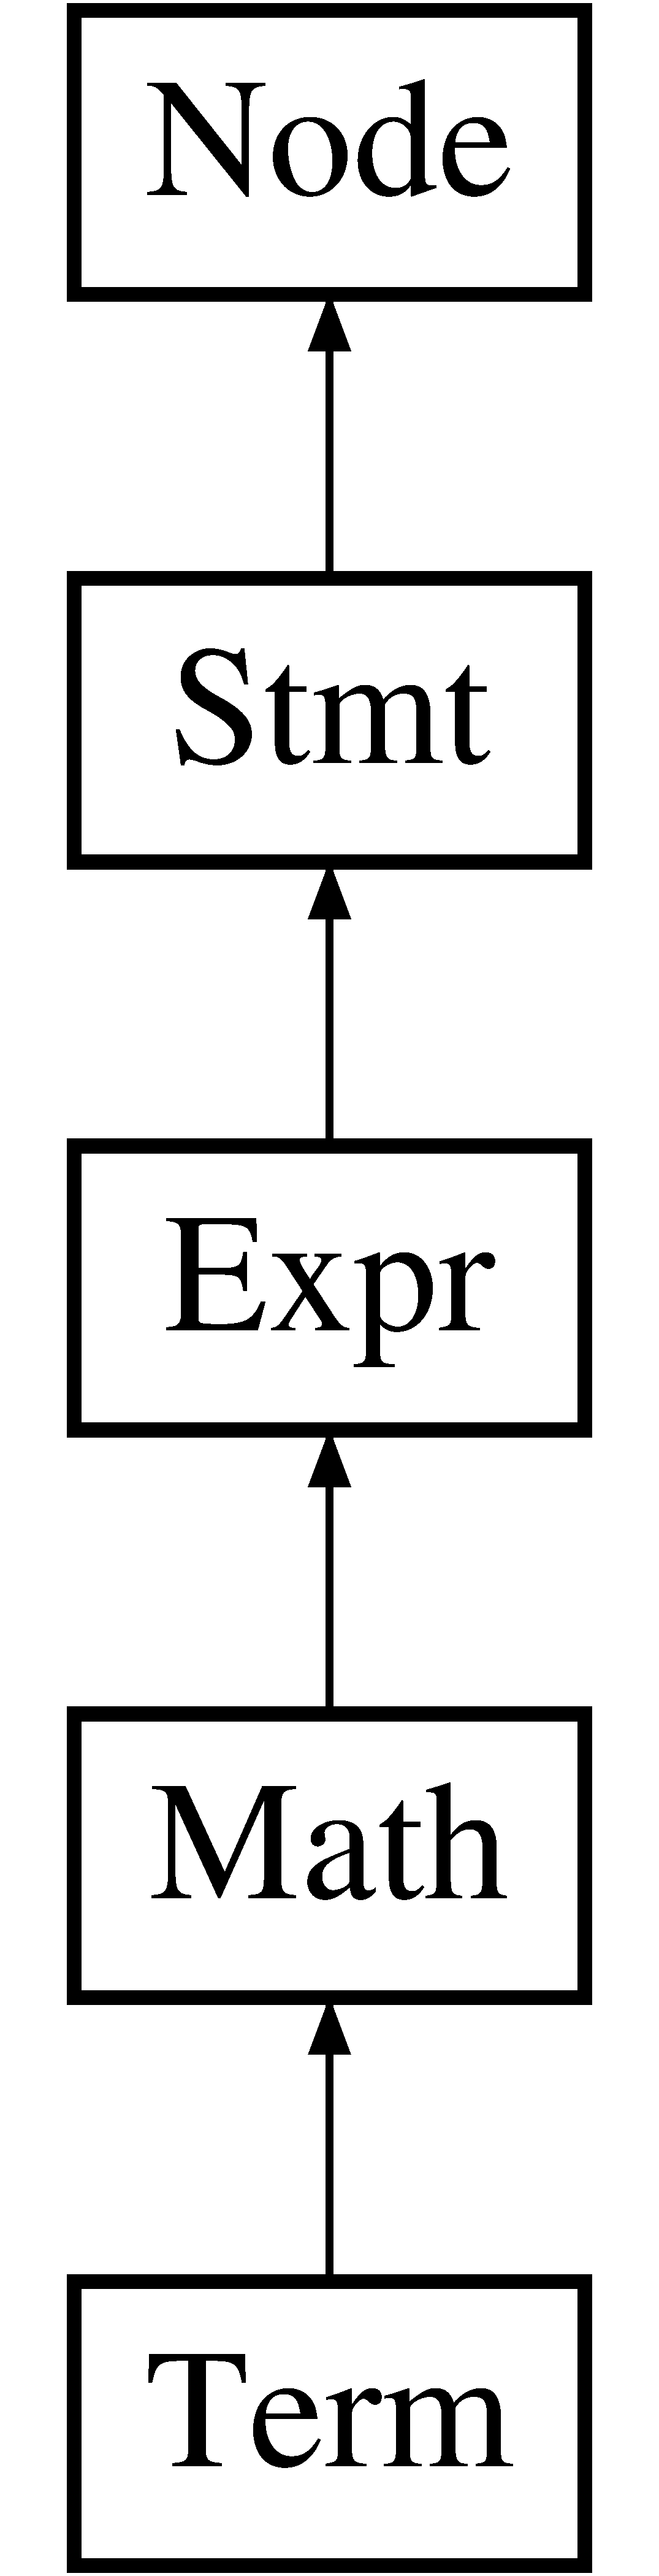
\includegraphics[height=5.000000cm]{class_term}
\end{center}
\end{figure}
\subsection*{Public 成员函数}
\begin{DoxyCompactItemize}
\item 
\hyperlink{class_term_aee8491368db463879893b7f374d5d835}{Term} (\hyperlink{class_token}{Token} $\ast$token, \hyperlink{class_expr}{Expr} $\ast$expr1, \hyperlink{class_expr}{Expr} $\ast$expr2)
\item 
\mbox{\Hypertarget{class_term_ac2d20115da73f9425e5d390856a211a1}\label{class_term_ac2d20115da73f9425e5d390856a211a1}} 
int \hyperlink{class_term_ac2d20115da73f9425e5d390856a211a1}{execute} ()
\begin{DoxyCompactList}\small\item\em 计算 \end{DoxyCompactList}\end{DoxyCompactItemize}
\subsection*{额外继承的成员函数}


\subsection{详细描述}
乘除运算符类 

\subsection{构造及析构函数说明}
\mbox{\Hypertarget{class_term_aee8491368db463879893b7f374d5d835}\label{class_term_aee8491368db463879893b7f374d5d835}} 
\index{Term@{Term}!Term@{Term}}
\index{Term@{Term}!Term@{Term}}
\subsubsection{\texorpdfstring{Term()}{Term()}}
{\footnotesize\ttfamily Term\+::\+Term (\begin{DoxyParamCaption}\item[{\hyperlink{class_token}{Token} $\ast$}]{token,  }\item[{\hyperlink{class_expr}{Expr} $\ast$}]{expr1,  }\item[{\hyperlink{class_expr}{Expr} $\ast$}]{expr2 }\end{DoxyParamCaption})}


\begin{DoxyParams}{参数}
{\em token} & \+: 运算符 \\
\hline
{\em expr1} & \+: 左表达式 \\
\hline
{\em expr2} & \+: 右表达式 \\
\hline
\end{DoxyParams}


该类的文档由以下文件生成\+:\begin{DoxyCompactItemize}
\item 
src/inter/stmt/expr/Term.\+h\item 
src/inter/stmt/expr/Term.\+cpp\end{DoxyCompactItemize}

\hypertarget{class_token}{}\section{Token类 参考}
\label{class_token}\index{Token@{Token}}


token类  




{\ttfamily \#include $<$Token.\+h$>$}

类 Token 继承关系图\+:\begin{figure}[H]
\begin{center}
\leavevmode
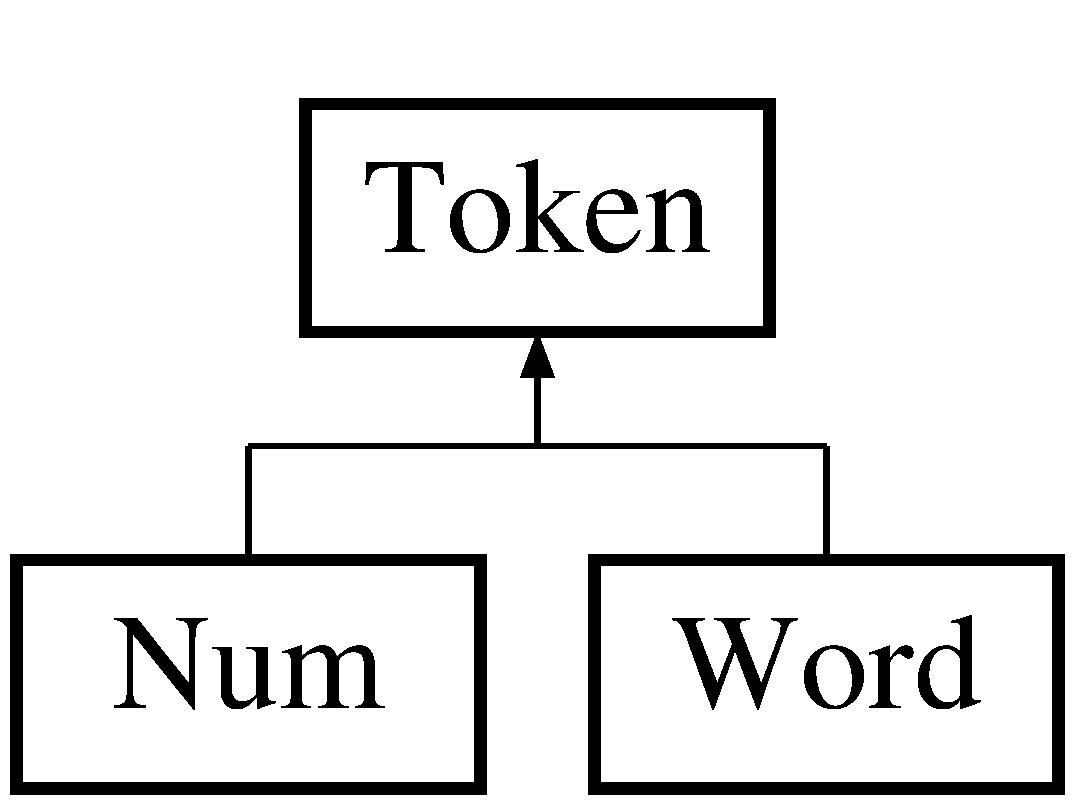
\includegraphics[height=2.000000cm]{class_token}
\end{center}
\end{figure}
\subsection*{Public 成员函数}
\begin{DoxyCompactItemize}
\item 
\hyperlink{class_token_a29580f176bfba9981aeec62946114675}{Token} (int t)
\item 
virtual std\+::string \hyperlink{class_token_a8863381edabce7bc1e92473b445ba81f}{to\+String} ()
\item 
bool \hyperlink{class_token_a157a63b83c2b18a64ba1f4170d476895}{operator$<$} (const \hyperlink{class_token}{Token} t) const \hypertarget{class_token_a157a63b83c2b18a64ba1f4170d476895}{}\label{class_token_a157a63b83c2b18a64ba1f4170d476895}

\begin{DoxyCompactList}\small\item\em 重载token的比较符,用于比较token \end{DoxyCompactList}\end{DoxyCompactItemize}
\subsection*{Public 属性}
\begin{DoxyCompactItemize}
\item 
int \hyperlink{class_token_a2a4b0e1b648c2a9be1976004eb3c4ff0}{tag}\hypertarget{class_token_a2a4b0e1b648c2a9be1976004eb3c4ff0}{}\label{class_token_a2a4b0e1b648c2a9be1976004eb3c4ff0}

\begin{DoxyCompactList}\small\item\em 该token的类型 \end{DoxyCompactList}\item 
int \hyperlink{class_token_a4b96c2a31d7c374fd2bd1986794f80dd}{line}
\end{DoxyCompactItemize}


\subsection{详细描述}
token类 

语法分析器中解析的基本元素 也是词法分析器中生成的元素 

\subsection{构造及析构函数说明}
\index{Token@{Token}!Token@{Token}}
\index{Token@{Token}!Token@{Token}}
\subsubsection[{\texorpdfstring{Token(int t)}{Token(int t)}}]{\setlength{\rightskip}{0pt plus 5cm}Token\+::\+Token (
\begin{DoxyParamCaption}
\item[{int}]{t}
\end{DoxyParamCaption}
)}\hypertarget{class_token_a29580f176bfba9981aeec62946114675}{}\label{class_token_a29580f176bfba9981aeec62946114675}

\begin{DoxyParams}{参数}
{\em t} & \+: 初始化token的tag值 \\
\hline
\end{DoxyParams}


\subsection{成员函数说明}
\index{Token@{Token}!to\+String@{to\+String}}
\index{to\+String@{to\+String}!Token@{Token}}
\subsubsection[{\texorpdfstring{to\+String()}{toString()}}]{\setlength{\rightskip}{0pt plus 5cm}std\+::string Token\+::to\+String (
\begin{DoxyParamCaption}
{}
\end{DoxyParamCaption}
)\hspace{0.3cm}{\ttfamily [virtual]}}\hypertarget{class_token_a8863381edabce7bc1e92473b445ba81f}{}\label{class_token_a8863381edabce7bc1e92473b445ba81f}
\begin{DoxyReturn}{返回}
返回该token的信息 
\end{DoxyReturn}


被 \hyperlink{class_word_a950a81bfd0fc369b0eb8d0d6b27e2870}{Word} , 以及 \hyperlink{class_num_aec8ab507b42f2080a8cc197f45f0c935}{Num} 重载.



\subsection{类成员变量说明}
\index{Token@{Token}!line@{line}}
\index{line@{line}!Token@{Token}}
\subsubsection[{\texorpdfstring{line}{line}}]{\setlength{\rightskip}{0pt plus 5cm}int Token\+::line}\hypertarget{class_token_a4b96c2a31d7c374fd2bd1986794f80dd}{}\label{class_token_a4b96c2a31d7c374fd2bd1986794f80dd}
该token所处的行号 

该类的文档由以下文件生成\+:\begin{DoxyCompactItemize}
\item 
src/lexer/Token.\+h\item 
src/lexer/Token.\+cpp\end{DoxyCompactItemize}

\hypertarget{class_unary}{}\section{Unary Class Reference}
\label{class_unary}\index{Unary@{Unary}}


正负运算符类  




{\ttfamily \#include $<$Unary.\+h$>$}

Inheritance diagram for Unary\+:\begin{figure}[H]
\begin{center}
\leavevmode
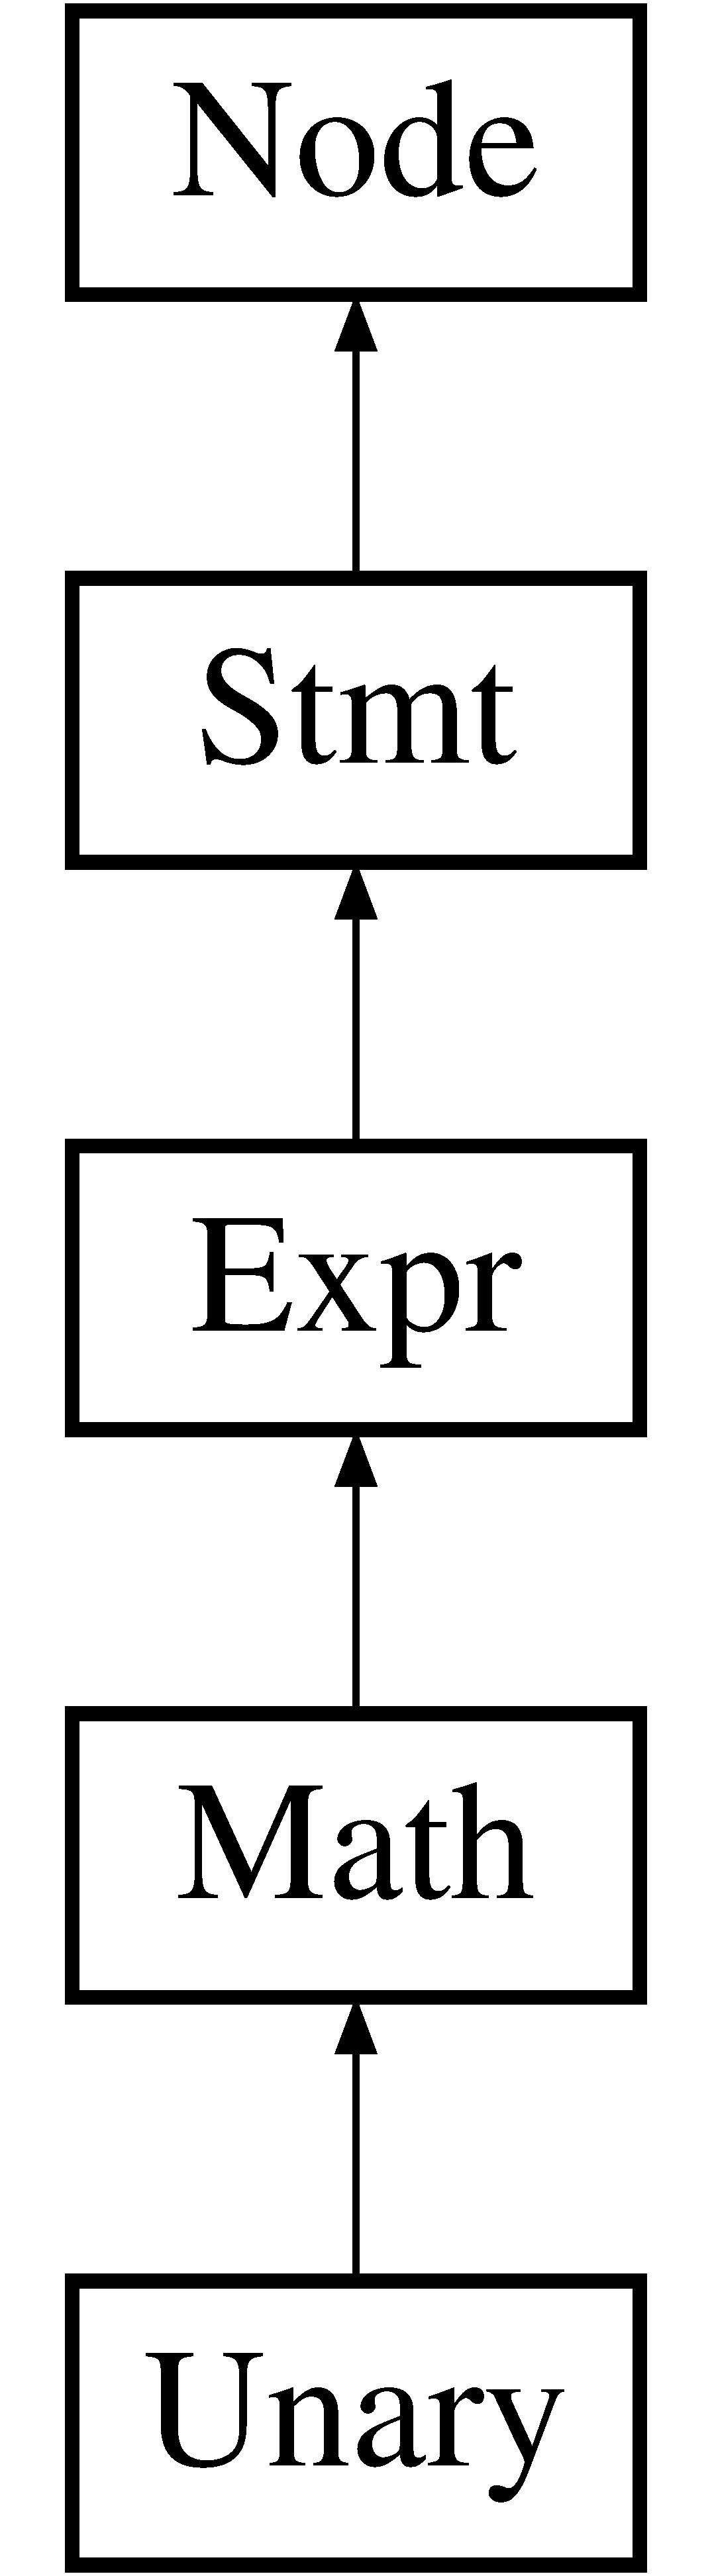
\includegraphics[height=5.000000cm]{class_unary}
\end{center}
\end{figure}
\subsection*{Public Member Functions}
\begin{DoxyCompactItemize}
\item 
\hyperlink{class_unary_ab8a81af2bbab768401579659ce929e53}{Unary} (\hyperlink{class_token}{Token} $\ast$, \hyperlink{class_expr}{Expr} $\ast$)
\item 
int \hyperlink{class_unary_af42edff1ee4718a9afeb7127e41af758}{execute} ()
\end{DoxyCompactItemize}
\subsection*{Additional Inherited Members}


\subsection{Detailed Description}
正负运算符类 

\subsection{Constructor \& Destructor Documentation}
\mbox{\Hypertarget{class_unary_ab8a81af2bbab768401579659ce929e53}\label{class_unary_ab8a81af2bbab768401579659ce929e53}} 
\index{Unary@{Unary}!Unary@{Unary}}
\index{Unary@{Unary}!Unary@{Unary}}
\subsubsection{\texorpdfstring{Unary()}{Unary()}}
{\footnotesize\ttfamily Unary\+::\+Unary (\begin{DoxyParamCaption}\item[{\hyperlink{class_token}{Token} $\ast$}]{token,  }\item[{\hyperlink{class_expr}{Expr} $\ast$}]{factor1 }\end{DoxyParamCaption})}


\begin{DoxyParams}{Parameters}
{\em token} & \+: 运算符 token \\
\hline
{\em expr} & \+: 被运算的表达式 \\
\hline
\end{DoxyParams}


\subsection{Member Function Documentation}
\mbox{\Hypertarget{class_unary_af42edff1ee4718a9afeb7127e41af758}\label{class_unary_af42edff1ee4718a9afeb7127e41af758}} 
\index{Unary@{Unary}!execute@{execute}}
\index{execute@{execute}!Unary@{Unary}}
\subsubsection{\texorpdfstring{execute()}{execute()}}
{\footnotesize\ttfamily int Unary\+::execute (\begin{DoxyParamCaption}{ }\end{DoxyParamCaption})\hspace{0.3cm}{\ttfamily [virtual]}}

\begin{DoxyReturn}{Returns}
返回正负号计算后的值 
\end{DoxyReturn}


Reimplemented from \hyperlink{class_expr_aff6a2e6eaa460e2a3db28ebdab089b51}{Expr}.



The documentation for this class was generated from the following files\+:\begin{DoxyCompactItemize}
\item 
src/inter/stmt/expr/\hyperlink{_unary_8h}{Unary.\+h}\item 
src/inter/stmt/expr/\hyperlink{_unary_8cpp}{Unary.\+cpp}\end{DoxyCompactItemize}

\hypertarget{class_var}{}\section{Var类 参考}
\label{class_var}\index{Var@{Var}}


变量类  




{\ttfamily \#include $<$Var.\+h$>$}

类 Var 继承关系图\+:\begin{figure}[H]
\begin{center}
\leavevmode
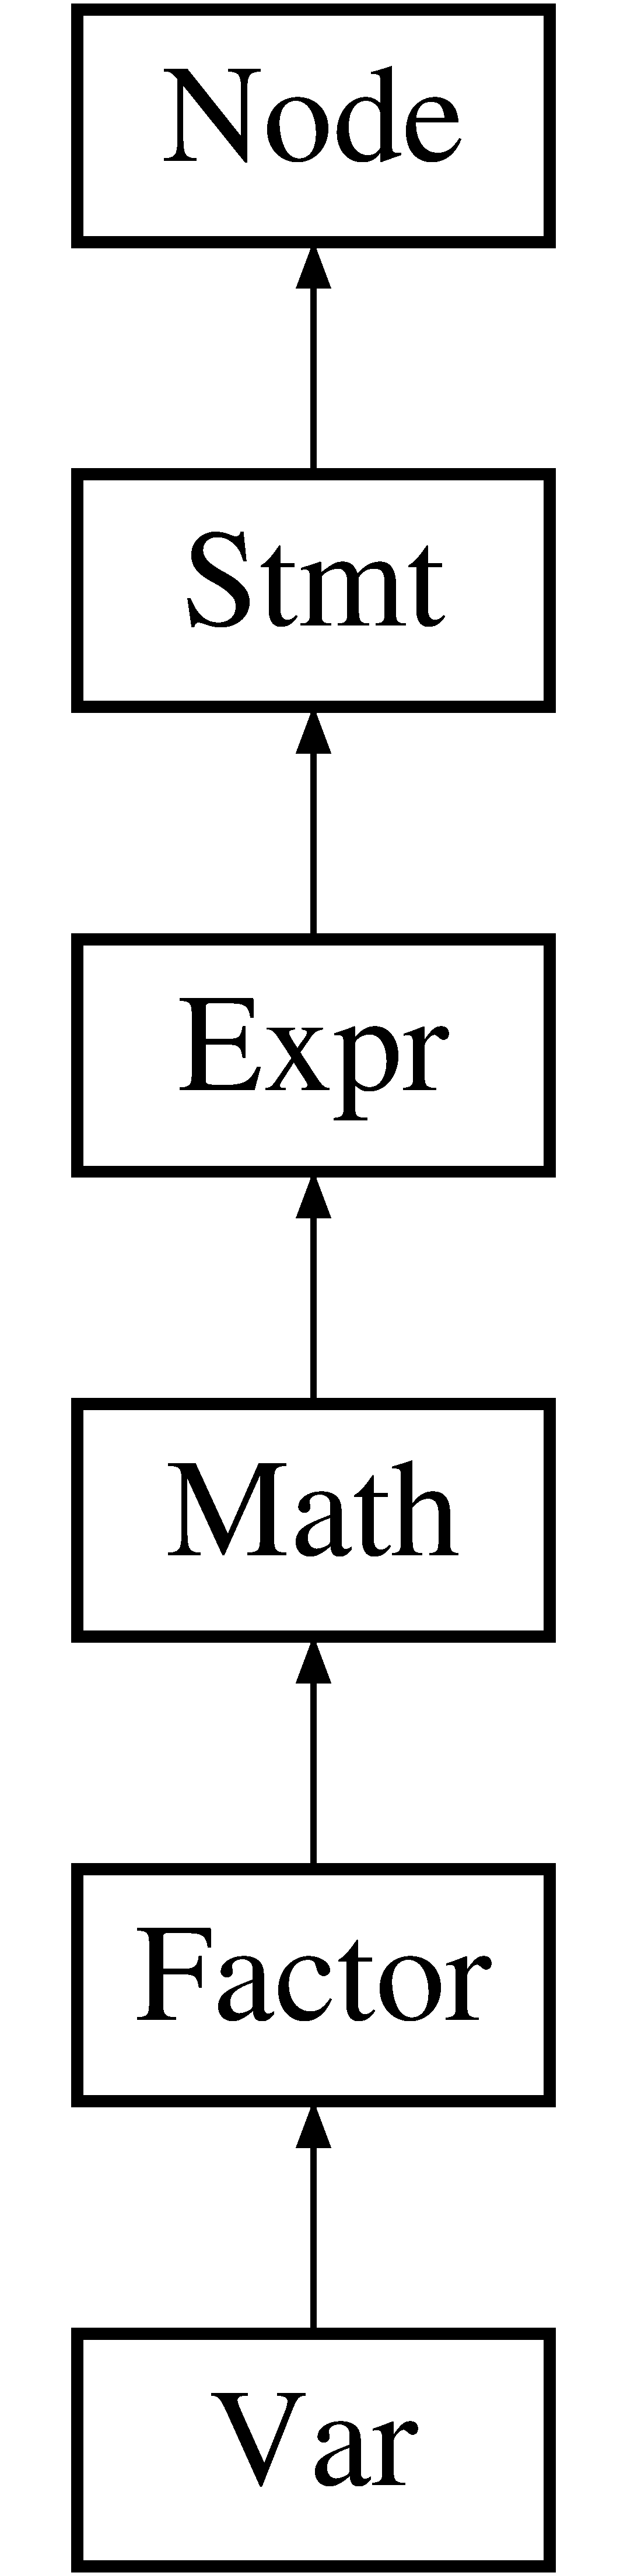
\includegraphics[height=6.000000cm]{class_var}
\end{center}
\end{figure}
\subsection*{Public 成员函数}
\begin{DoxyCompactItemize}
\item 
bool \hyperlink{class_var_a50aa6f54310903a8bc36184813a2b9ef}{is\+Var} ()
\item 
{\bfseries Var} (\hyperlink{class_word}{Word} $\ast$)\hypertarget{class_var_ab111df39c1575d7ba1f96f3b89574b8c}{}\label{class_var_ab111df39c1575d7ba1f96f3b89574b8c}

\item 
int \hyperlink{class_var_a9dc96e803f7b0f9aa519c2c0e0a6bd8f}{execute} ()
\item 
void \hyperlink{class_var_af0f42d31f5001ff4d4781b9ba199a612}{set\+Value} (int)\hypertarget{class_var_af0f42d31f5001ff4d4781b9ba199a612}{}\label{class_var_af0f42d31f5001ff4d4781b9ba199a612}

\begin{DoxyCompactList}\small\item\em 设置变量的值 \end{DoxyCompactList}\end{DoxyCompactItemize}
\subsection*{Public 属性}
\begin{DoxyCompactItemize}
\item 
\hyperlink{class_id}{Id} $\ast$ \hyperlink{class_var_a3e5c7c9425da4659290da5c0553c7dc6}{id}
\end{DoxyCompactItemize}
\subsection*{额外继承的成员函数}


\subsection{详细描述}
变量类 

\subsection{成员函数说明}
\index{Var@{Var}!execute@{execute}}
\index{execute@{execute}!Var@{Var}}
\subsubsection[{\texorpdfstring{execute()}{execute()}}]{\setlength{\rightskip}{0pt plus 5cm}int Var\+::execute (
\begin{DoxyParamCaption}
{}
\end{DoxyParamCaption}
)\hspace{0.3cm}{\ttfamily [virtual]}}\hypertarget{class_var_a9dc96e803f7b0f9aa519c2c0e0a6bd8f}{}\label{class_var_a9dc96e803f7b0f9aa519c2c0e0a6bd8f}
\begin{DoxyReturn}{返回}
变量的值 
\end{DoxyReturn}


重载 \hyperlink{class_expr_aff6a2e6eaa460e2a3db28ebdab089b51}{Expr} .

\index{Var@{Var}!is\+Var@{is\+Var}}
\index{is\+Var@{is\+Var}!Var@{Var}}
\subsubsection[{\texorpdfstring{is\+Var()}{isVar()}}]{\setlength{\rightskip}{0pt plus 5cm}bool Var\+::is\+Var (
\begin{DoxyParamCaption}
{}
\end{DoxyParamCaption}
)\hspace{0.3cm}{\ttfamily [virtual]}}\hypertarget{class_var_a50aa6f54310903a8bc36184813a2b9ef}{}\label{class_var_a50aa6f54310903a8bc36184813a2b9ef}

\begin{DoxyParams}{参数}
{\em word} & \+: 变量名的 token \\
\hline
\end{DoxyParams}


重载 \hyperlink{class_expr}{Expr} .



\subsection{类成员变量说明}
\index{Var@{Var}!id@{id}}
\index{id@{id}!Var@{Var}}
\subsubsection[{\texorpdfstring{id}{id}}]{\setlength{\rightskip}{0pt plus 5cm}{\bf Id}$\ast$ Var\+::id}\hypertarget{class_var_a3e5c7c9425da4659290da5c0553c7dc6}{}\label{class_var_a3e5c7c9425da4659290da5c0553c7dc6}
作用域的内的id 

该类的文档由以下文件生成\+:\begin{DoxyCompactItemize}
\item 
src/inter/stmt/expr/Var.\+h\item 
src/inter/stmt/expr/Var.\+cpp\end{DoxyCompactItemize}

\hypertarget{class_var_not_found}{}\section{Var\+Not\+Found Class Reference}
\label{class_var_not_found}\index{Var\+Not\+Found@{Var\+Not\+Found}}


{\ttfamily \#include $<$Var\+Not\+Found.\+h$>$}

Inheritance diagram for Var\+Not\+Found\+:\begin{figure}[H]
\begin{center}
\leavevmode
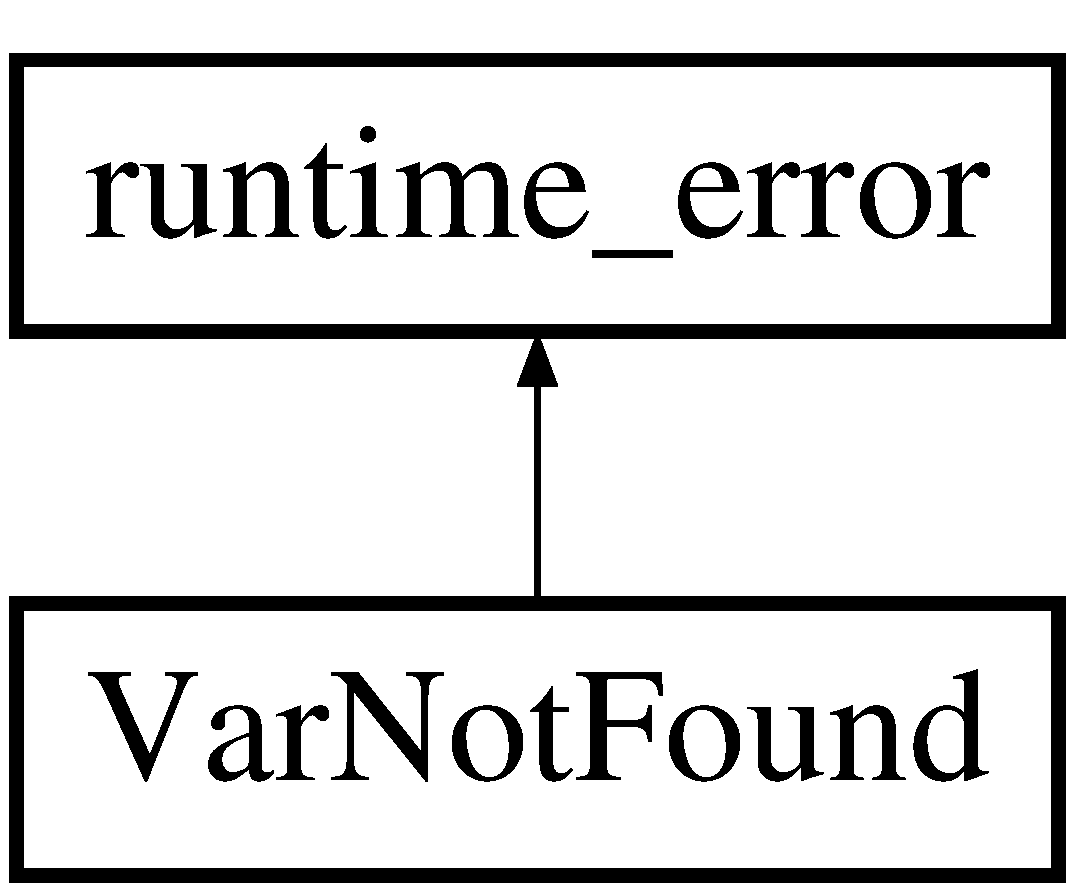
\includegraphics[height=2.000000cm]{class_var_not_found}
\end{center}
\end{figure}
\subsection*{Public Member Functions}
\begin{DoxyCompactItemize}
\item 
\hyperlink{class_var_not_found_a36600e0d18a90f6a594cb582940b5bbc}{Var\+Not\+Found} (std\+::string)
\end{DoxyCompactItemize}


\subsection{Constructor \& Destructor Documentation}
\mbox{\Hypertarget{class_var_not_found_a36600e0d18a90f6a594cb582940b5bbc}\label{class_var_not_found_a36600e0d18a90f6a594cb582940b5bbc}} 
\index{Var\+Not\+Found@{Var\+Not\+Found}!Var\+Not\+Found@{Var\+Not\+Found}}
\index{Var\+Not\+Found@{Var\+Not\+Found}!Var\+Not\+Found@{Var\+Not\+Found}}
\subsubsection{\texorpdfstring{Var\+Not\+Found()}{VarNotFound()}}
{\footnotesize\ttfamily Var\+Not\+Found\+::\+Var\+Not\+Found (\begin{DoxyParamCaption}\item[{std\+::string}]{s }\end{DoxyParamCaption})\hspace{0.3cm}{\ttfamily [explicit]}}



The documentation for this class was generated from the following files\+:\begin{DoxyCompactItemize}
\item 
src/inter/error/\hyperlink{_var_not_found_8h}{Var\+Not\+Found.\+h}\item 
src/inter/error/\hyperlink{_var_not_found_8cpp}{Var\+Not\+Found.\+cpp}\end{DoxyCompactItemize}

\hypertarget{class_var_not_inited}{}\section{Var\+Not\+Inited Class Reference}
\label{class_var_not_inited}\index{Var\+Not\+Inited@{Var\+Not\+Inited}}


{\ttfamily \#include $<$Var\+Not\+Inited.\+h$>$}

Inheritance diagram for Var\+Not\+Inited\+:\begin{figure}[H]
\begin{center}
\leavevmode
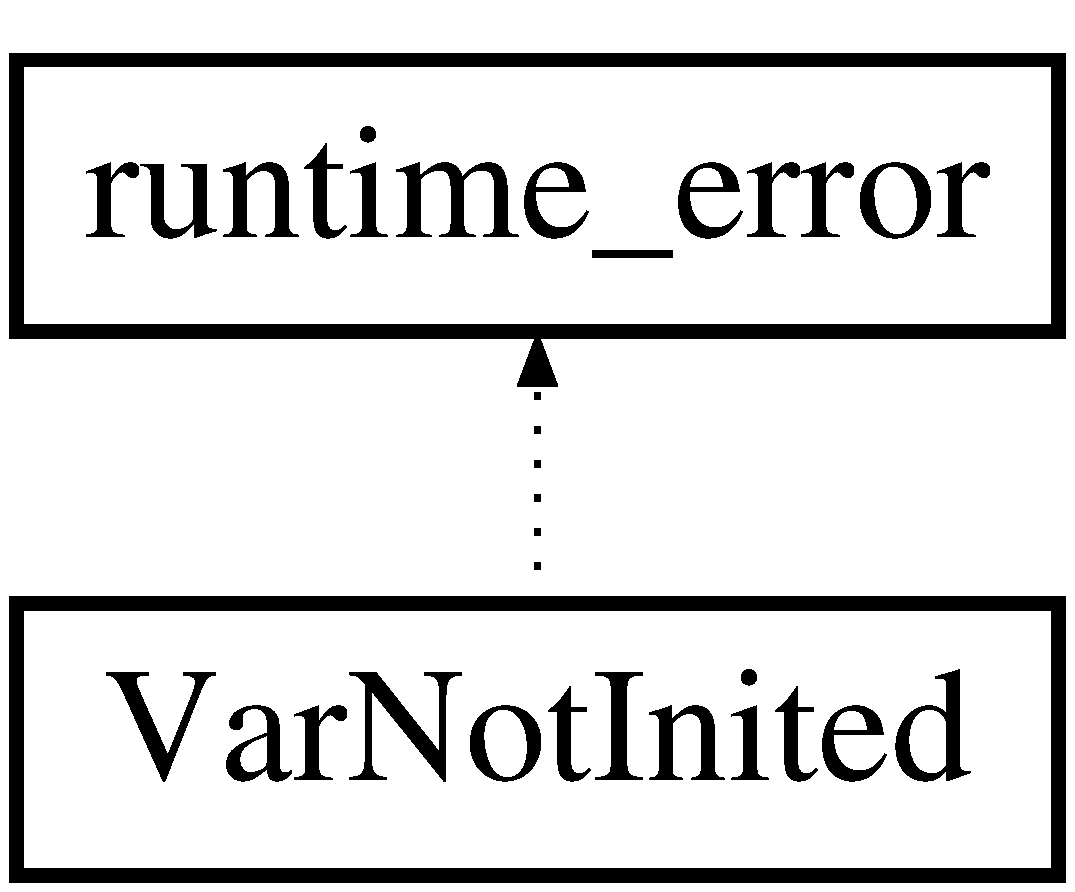
\includegraphics[height=2.000000cm]{class_var_not_inited}
\end{center}
\end{figure}
\subsection*{Public Member Functions}
\begin{DoxyCompactItemize}
\item 
\hyperlink{class_var_not_inited_a14d78a6013df47440f2eba2074c1ef62}{Var\+Not\+Inited} (std\+::string)
\end{DoxyCompactItemize}


\subsection{Constructor \& Destructor Documentation}
\mbox{\Hypertarget{class_var_not_inited_a14d78a6013df47440f2eba2074c1ef62}\label{class_var_not_inited_a14d78a6013df47440f2eba2074c1ef62}} 
\index{Var\+Not\+Inited@{Var\+Not\+Inited}!Var\+Not\+Inited@{Var\+Not\+Inited}}
\index{Var\+Not\+Inited@{Var\+Not\+Inited}!Var\+Not\+Inited@{Var\+Not\+Inited}}
\subsubsection{\texorpdfstring{Var\+Not\+Inited()}{VarNotInited()}}
{\footnotesize\ttfamily Var\+Not\+Inited\+::\+Var\+Not\+Inited (\begin{DoxyParamCaption}\item[{std\+::string}]{s }\end{DoxyParamCaption})\hspace{0.3cm}{\ttfamily [explicit]}}



The documentation for this class was generated from the following files\+:\begin{DoxyCompactItemize}
\item 
src/inter/error/\hyperlink{_var_not_inited_8h}{Var\+Not\+Inited.\+h}\item 
src/inter/error/\hyperlink{_var_not_inited_8cpp}{Var\+Not\+Inited.\+cpp}\end{DoxyCompactItemize}

\hypertarget{class_vm}{}\section{Vm Class Reference}
\label{class_vm}\index{Vm@{Vm}}


虚拟机类  




{\ttfamily \#include $<$Vm.\+h$>$}

\subsection*{Public Member Functions}
\begin{DoxyCompactItemize}
\item 
void \hyperlink{class_vm_a37a0791ef2b63e41421446993d0e7e4d}{execute} ()
\begin{DoxyCompactList}\small\item\em 执行整个语法树 \end{DoxyCompactList}\item 
void \hyperlink{class_vm_af036edc52fab207ca28530c06b6d0c67}{set\+Entry} (\hyperlink{class_block}{Block} $\ast$)
\begin{DoxyCompactList}\small\item\em 设置语法树入口 \end{DoxyCompactList}\item 
\hyperlink{class_vm_a4a37106b5b5b9382baa79dea901db8ba}{Vm} (\hyperlink{class_block}{Block} $\ast$)
\end{DoxyCompactItemize}
\subsection*{Static Public Member Functions}
\begin{DoxyCompactItemize}
\item 
static void \hyperlink{class_vm_a376141bb4182218ac7a499043eb18a6c}{print\+Line} (int line\+Number)
\begin{DoxyCompactList}\small\item\em 输出行号 \end{DoxyCompactList}\end{DoxyCompactItemize}
\subsection*{Static Public Attributes}
\begin{DoxyCompactItemize}
\item 
static \hyperlink{class_env}{Env} $\ast$ \hyperlink{class_vm_a1a83823801a5ab090d9ad20527a6c638}{top}
\end{DoxyCompactItemize}
\subsection*{Protected Attributes}
\begin{DoxyCompactItemize}
\item 
\hyperlink{class_block}{Block} $\ast$ \hyperlink{class_vm_ab5aae972ea15ddfd01362e27ed797a51}{entry}
\begin{DoxyCompactList}\small\item\em 语法树的入口 \end{DoxyCompactList}\end{DoxyCompactItemize}
\subsection*{Static Private Attributes}
\begin{DoxyCompactItemize}
\item 
static int \hyperlink{class_vm_acfa435ede93d1ba8fe2250fd3469de15}{current\+Line} = 0
\begin{DoxyCompactList}\small\item\em 运行到的当前行 \end{DoxyCompactList}\end{DoxyCompactItemize}


\subsection{Detailed Description}
虚拟机类 

用于执行整个抽象语法树 

\subsection{Constructor \& Destructor Documentation}
\mbox{\Hypertarget{class_vm_a4a37106b5b5b9382baa79dea901db8ba}\label{class_vm_a4a37106b5b5b9382baa79dea901db8ba}} 
\index{Vm@{Vm}!Vm@{Vm}}
\index{Vm@{Vm}!Vm@{Vm}}
\subsubsection{\texorpdfstring{Vm()}{Vm()}}
{\footnotesize\ttfamily Vm\+::\+Vm (\begin{DoxyParamCaption}\item[{\hyperlink{class_block}{Block} $\ast$}]{node }\end{DoxyParamCaption})}


\begin{DoxyParams}{Parameters}
{\em block} & \+: 程序运行的初始block \\
\hline
\end{DoxyParams}


\subsection{Member Function Documentation}
\mbox{\Hypertarget{class_vm_a37a0791ef2b63e41421446993d0e7e4d}\label{class_vm_a37a0791ef2b63e41421446993d0e7e4d}} 
\index{Vm@{Vm}!execute@{execute}}
\index{execute@{execute}!Vm@{Vm}}
\subsubsection{\texorpdfstring{execute()}{execute()}}
{\footnotesize\ttfamily void Vm\+::execute (\begin{DoxyParamCaption}{ }\end{DoxyParamCaption})}



执行整个语法树 

\mbox{\Hypertarget{class_vm_a376141bb4182218ac7a499043eb18a6c}\label{class_vm_a376141bb4182218ac7a499043eb18a6c}} 
\index{Vm@{Vm}!print\+Line@{print\+Line}}
\index{print\+Line@{print\+Line}!Vm@{Vm}}
\subsubsection{\texorpdfstring{print\+Line()}{printLine()}}
{\footnotesize\ttfamily void Vm\+::print\+Line (\begin{DoxyParamCaption}\item[{int}]{line\+Number }\end{DoxyParamCaption})\hspace{0.3cm}{\ttfamily [static]}}



输出行号 

\mbox{\Hypertarget{class_vm_af036edc52fab207ca28530c06b6d0c67}\label{class_vm_af036edc52fab207ca28530c06b6d0c67}} 
\index{Vm@{Vm}!set\+Entry@{set\+Entry}}
\index{set\+Entry@{set\+Entry}!Vm@{Vm}}
\subsubsection{\texorpdfstring{set\+Entry()}{setEntry()}}
{\footnotesize\ttfamily void Vm\+::set\+Entry (\begin{DoxyParamCaption}\item[{\hyperlink{class_block}{Block} $\ast$}]{node }\end{DoxyParamCaption})}



设置语法树入口 



\subsection{Member Data Documentation}
\mbox{\Hypertarget{class_vm_acfa435ede93d1ba8fe2250fd3469de15}\label{class_vm_acfa435ede93d1ba8fe2250fd3469de15}} 
\index{Vm@{Vm}!current\+Line@{current\+Line}}
\index{current\+Line@{current\+Line}!Vm@{Vm}}
\subsubsection{\texorpdfstring{current\+Line}{currentLine}}
{\footnotesize\ttfamily int Vm\+::current\+Line = 0\hspace{0.3cm}{\ttfamily [static]}, {\ttfamily [private]}}



运行到的当前行 

\mbox{\Hypertarget{class_vm_ab5aae972ea15ddfd01362e27ed797a51}\label{class_vm_ab5aae972ea15ddfd01362e27ed797a51}} 
\index{Vm@{Vm}!entry@{entry}}
\index{entry@{entry}!Vm@{Vm}}
\subsubsection{\texorpdfstring{entry}{entry}}
{\footnotesize\ttfamily \hyperlink{class_block}{Block}$\ast$ Vm\+::entry\hspace{0.3cm}{\ttfamily [protected]}}



语法树的入口 

\mbox{\Hypertarget{class_vm_a1a83823801a5ab090d9ad20527a6c638}\label{class_vm_a1a83823801a5ab090d9ad20527a6c638}} 
\index{Vm@{Vm}!top@{top}}
\index{top@{top}!Vm@{Vm}}
\subsubsection{\texorpdfstring{top}{top}}
{\footnotesize\ttfamily \hyperlink{class_env}{Env} $\ast$ Vm\+::top\hspace{0.3cm}{\ttfamily [static]}}

当前运行的变量环境 

The documentation for this class was generated from the following files\+:\begin{DoxyCompactItemize}
\item 
src/vm/\hyperlink{_vm_8h}{Vm.\+h}\item 
src/vm/\hyperlink{_vm_8cpp}{Vm.\+cpp}\end{DoxyCompactItemize}

\hypertarget{class_while}{}\section{While Class Reference}
\label{class_while}\index{While@{While}}


{\ttfamily \#include $<$While.\+h$>$}

Inheritance diagram for While\+:\begin{figure}[H]
\begin{center}
\leavevmode
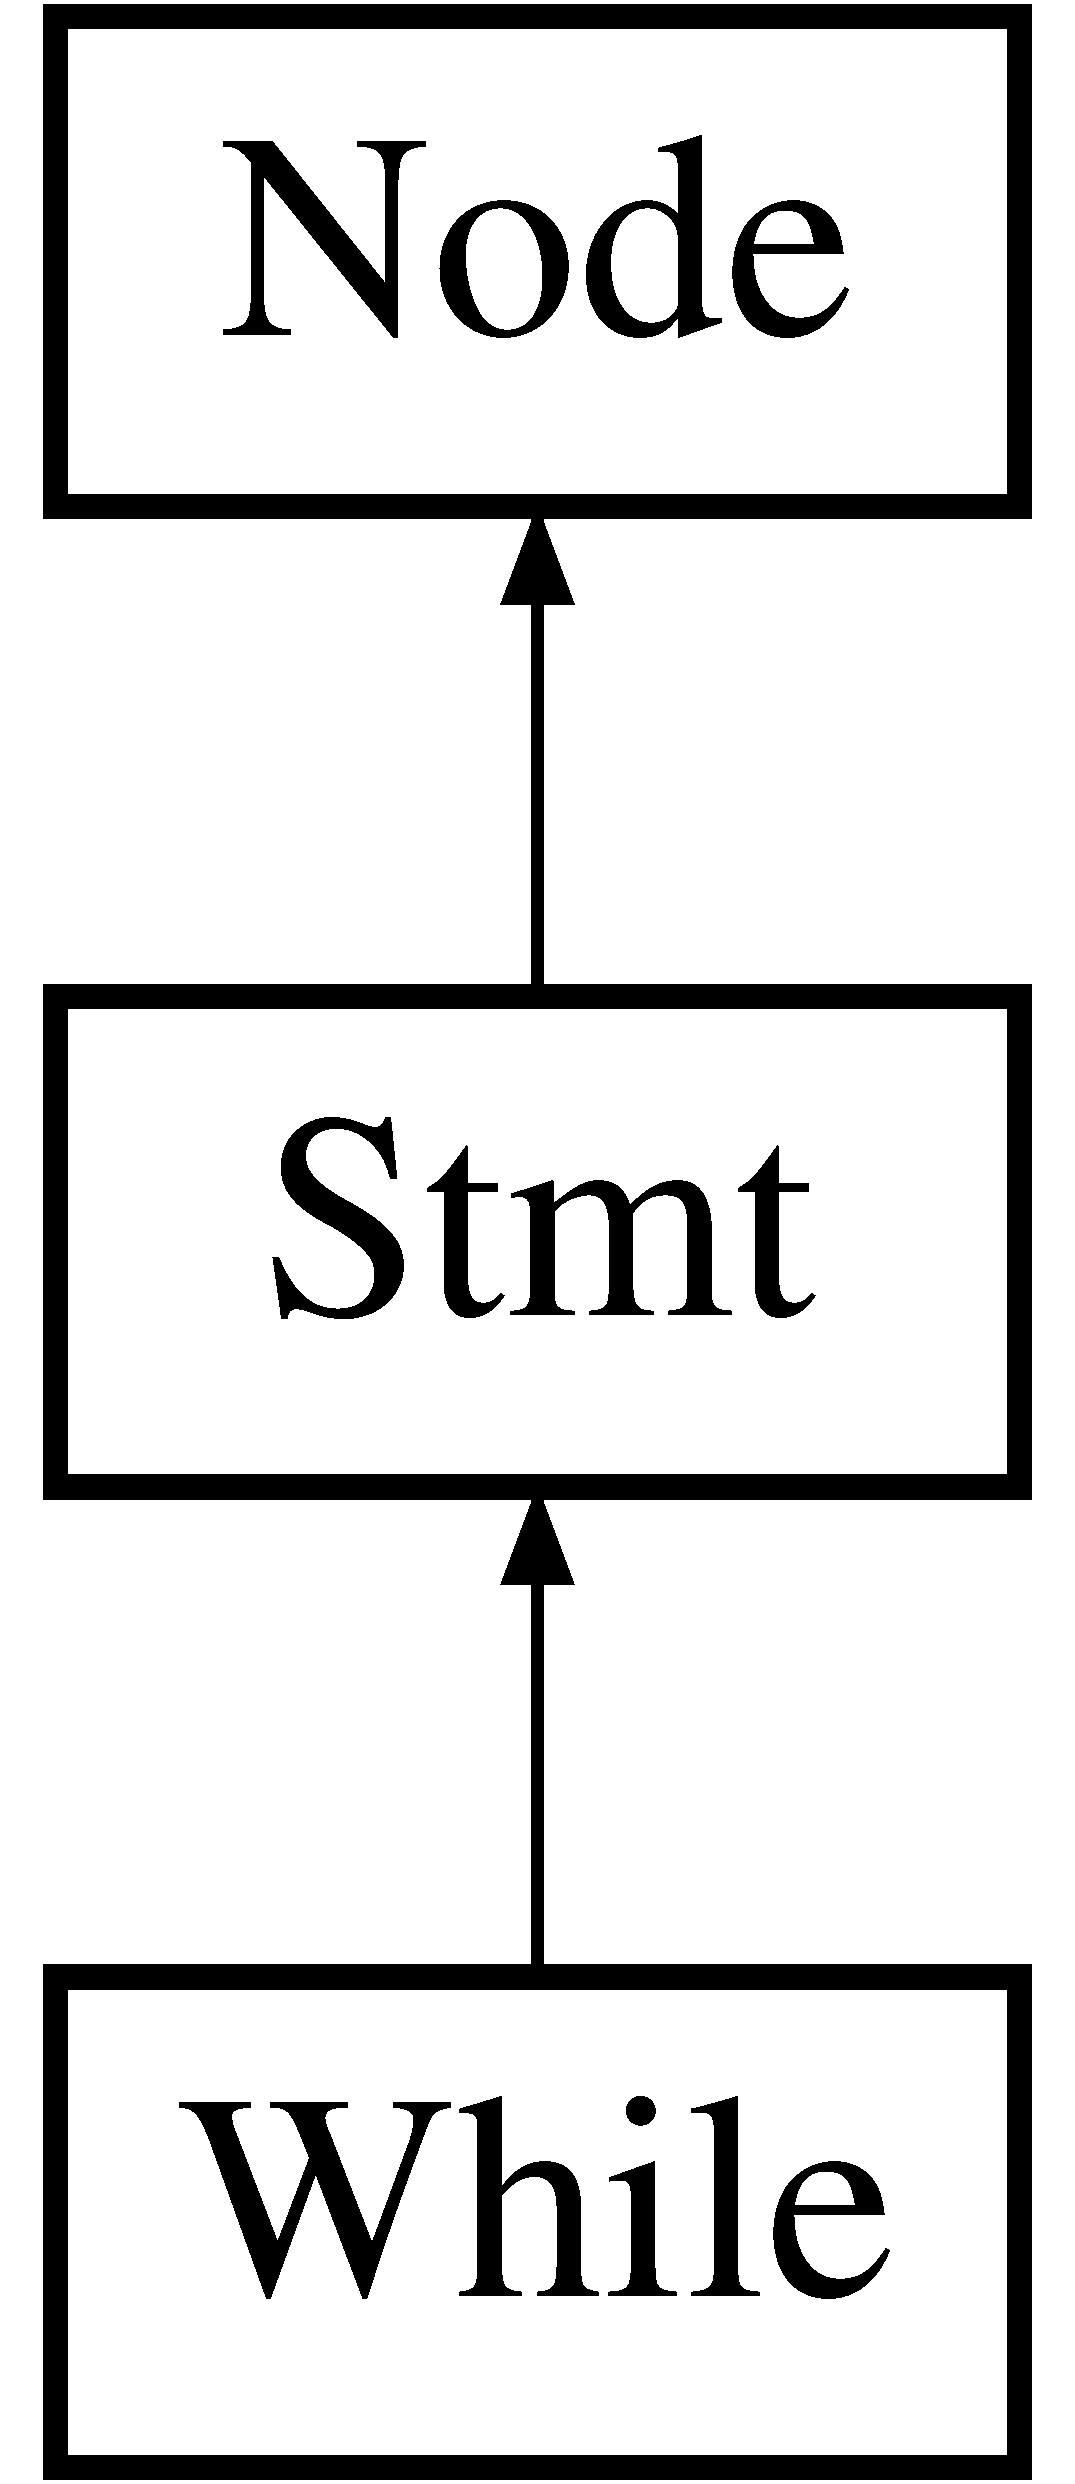
\includegraphics[height=3.000000cm]{class_while}
\end{center}
\end{figure}
\subsection*{Public Member Functions}
\begin{DoxyCompactItemize}
\item 
\hyperlink{class_while_aacee45c95a102a5a1ec711bbc29c92a7}{While} ()
\item 
int \hyperlink{class_while_a23b58565983130bb54577f4399ffd822}{execute} ()
\begin{DoxyCompactList}\small\item\em 抽象的执行方法 \end{DoxyCompactList}\end{DoxyCompactItemize}
\subsection*{Public Attributes}
\begin{DoxyCompactItemize}
\item 
\hyperlink{class_expr}{Expr} $\ast$ \hyperlink{class_while_a14af77714254099c0cc465944ef67dd3}{equality} = N\+U\+LL
\item 
\hyperlink{class_stmt}{Stmt} $\ast$ \hyperlink{class_while_a97dfbf50f27b969c5b765ecfb1ef4ac2}{stmt} = N\+U\+LL
\end{DoxyCompactItemize}
\subsection*{Additional Inherited Members}


\subsection{Constructor \& Destructor Documentation}
\mbox{\Hypertarget{class_while_aacee45c95a102a5a1ec711bbc29c92a7}\label{class_while_aacee45c95a102a5a1ec711bbc29c92a7}} 
\index{While@{While}!While@{While}}
\index{While@{While}!While@{While}}
\subsubsection{\texorpdfstring{While()}{While()}}
{\footnotesize\ttfamily While\+::\+While (\begin{DoxyParamCaption}{ }\end{DoxyParamCaption})\hspace{0.3cm}{\ttfamily [inline]}}



\subsection{Member Function Documentation}
\mbox{\Hypertarget{class_while_a23b58565983130bb54577f4399ffd822}\label{class_while_a23b58565983130bb54577f4399ffd822}} 
\index{While@{While}!execute@{execute}}
\index{execute@{execute}!While@{While}}
\subsubsection{\texorpdfstring{execute()}{execute()}}
{\footnotesize\ttfamily int While\+::execute (\begin{DoxyParamCaption}{ }\end{DoxyParamCaption})\hspace{0.3cm}{\ttfamily [virtual]}}



抽象的执行方法 

因为表达式以及各种语句都是可执行的~\newline
设立这个方法利用多态可以实现整个语法树的执行~\newline
 \begin{DoxyReturn}{Returns}
int \+: 表达式或语句执行后获得的值 
\end{DoxyReturn}


Reimplemented from \hyperlink{class_stmt_abdc3261770c3c5bd3ce5b3ba6eedfaa4}{Stmt}.



\subsection{Member Data Documentation}
\mbox{\Hypertarget{class_while_a14af77714254099c0cc465944ef67dd3}\label{class_while_a14af77714254099c0cc465944ef67dd3}} 
\index{While@{While}!equality@{equality}}
\index{equality@{equality}!While@{While}}
\subsubsection{\texorpdfstring{equality}{equality}}
{\footnotesize\ttfamily \hyperlink{class_expr}{Expr}$\ast$ While\+::equality = N\+U\+LL}

\mbox{\Hypertarget{class_while_a97dfbf50f27b969c5b765ecfb1ef4ac2}\label{class_while_a97dfbf50f27b969c5b765ecfb1ef4ac2}} 
\index{While@{While}!stmt@{stmt}}
\index{stmt@{stmt}!While@{While}}
\subsubsection{\texorpdfstring{stmt}{stmt}}
{\footnotesize\ttfamily \hyperlink{class_stmt}{Stmt}$\ast$ While\+::stmt = N\+U\+LL}



The documentation for this class was generated from the following files\+:\begin{DoxyCompactItemize}
\item 
src/inter/stmt/\hyperlink{_while_8h}{While.\+h}\item 
src/inter/stmt/\hyperlink{_while_8cpp}{While.\+cpp}\end{DoxyCompactItemize}

\hypertarget{class_word}{}\section{Word Class Reference}
\label{class_word}\index{Word@{Word}}


字类  




{\ttfamily \#include $<$Word.\+h$>$}

Inheritance diagram for Word\+:\begin{figure}[H]
\begin{center}
\leavevmode
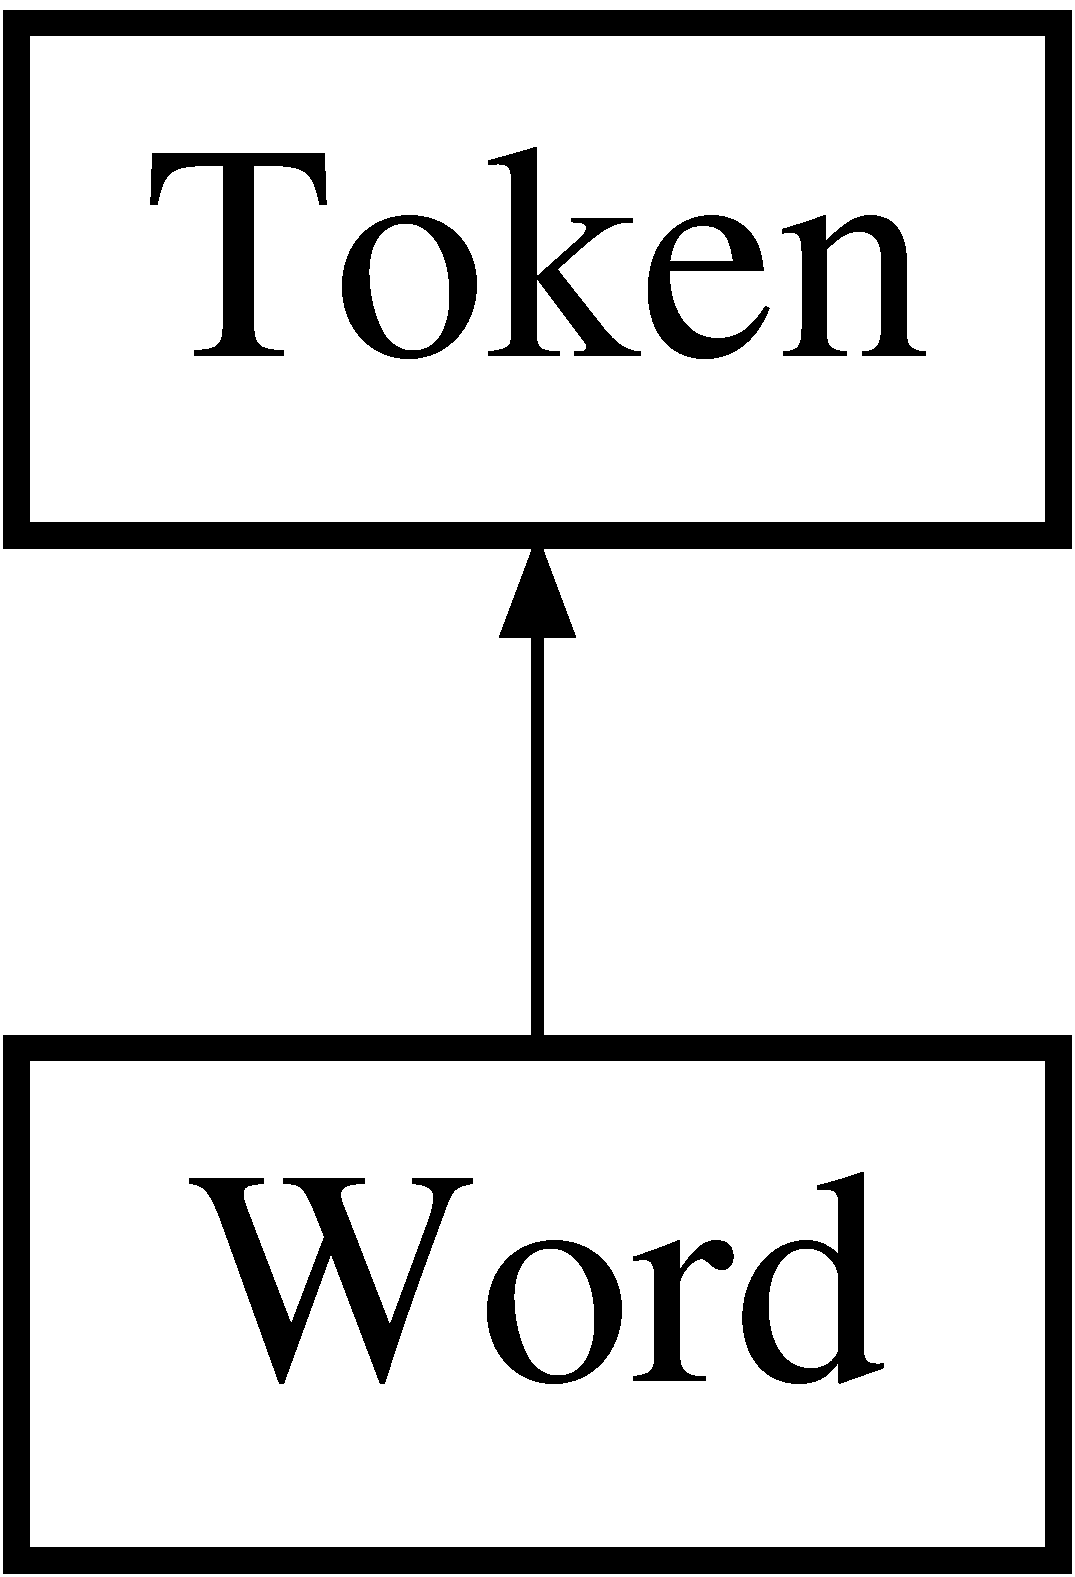
\includegraphics[height=2.000000cm]{class_word}
\end{center}
\end{figure}
\subsection*{Public Member Functions}
\begin{DoxyCompactItemize}
\item 
\hyperlink{class_word_acb127ce0ab789dc0ecfc407dec786ac2}{Word} (std\+::string s, int \hyperlink{class_token_a2a4b0e1b648c2a9be1976004eb3c4ff0}{tag})
\item 
std\+::string \hyperlink{class_word_a950a81bfd0fc369b0eb8d0d6b27e2870}{to\+String} ()
\end{DoxyCompactItemize}
\subsection*{Public Attributes}
\begin{DoxyCompactItemize}
\item 
std\+::string \hyperlink{class_word_a34691d869ec57b2a0b7a8eb41230b92a}{lexeme} = \char`\"{}\char`\"{}
\end{DoxyCompactItemize}


\subsection{Detailed Description}
字类 

代表关键字, 变量名等的 对应类 

\subsection{Constructor \& Destructor Documentation}
\mbox{\Hypertarget{class_word_acb127ce0ab789dc0ecfc407dec786ac2}\label{class_word_acb127ce0ab789dc0ecfc407dec786ac2}} 
\index{Word@{Word}!Word@{Word}}
\index{Word@{Word}!Word@{Word}}
\subsubsection{\texorpdfstring{Word()}{Word()}}
{\footnotesize\ttfamily Word\+::\+Word (\begin{DoxyParamCaption}\item[{std\+::string}]{s,  }\item[{int}]{tag }\end{DoxyParamCaption})}


\begin{DoxyParams}{Parameters}
{\em s} & \+: 该字的字符串 \\
\hline
{\em tag} & \+: 该字的类型 \\
\hline
\end{DoxyParams}


\subsection{Member Function Documentation}
\mbox{\Hypertarget{class_word_a950a81bfd0fc369b0eb8d0d6b27e2870}\label{class_word_a950a81bfd0fc369b0eb8d0d6b27e2870}} 
\index{Word@{Word}!to\+String@{to\+String}}
\index{to\+String@{to\+String}!Word@{Word}}
\subsubsection{\texorpdfstring{to\+String()}{toString()}}
{\footnotesize\ttfamily std\+::string Word\+::to\+String (\begin{DoxyParamCaption}{ }\end{DoxyParamCaption})\hspace{0.3cm}{\ttfamily [virtual]}}

将字输出成字符串 \begin{DoxyReturn}{Returns}
该字的字符串 
\end{DoxyReturn}


Reimplemented from \hyperlink{class_token_a8863381edabce7bc1e92473b445ba81f}{Token}.



\subsection{Member Data Documentation}
\mbox{\Hypertarget{class_word_a34691d869ec57b2a0b7a8eb41230b92a}\label{class_word_a34691d869ec57b2a0b7a8eb41230b92a}} 
\index{Word@{Word}!lexeme@{lexeme}}
\index{lexeme@{lexeme}!Word@{Word}}
\subsubsection{\texorpdfstring{lexeme}{lexeme}}
{\footnotesize\ttfamily std\+::string Word\+::lexeme = \char`\"{}\char`\"{}}

改字的字符串信息 

The documentation for this class was generated from the following files\+:\begin{DoxyCompactItemize}
\item 
src/lexer/Word.\+h\item 
src/lexer/Word.\+cpp\end{DoxyCompactItemize}

%--- End generated contents ---

% Index
\backmatter
\newpage
\phantomsection
\clearemptydoublepage
\addcontentsline{toc}{chapter}{索引}
\printindex

\end{document}
